% for %f in (*.pdf) do pdfcrop "%f" "%f"
% pdfcrop your_file.pdf output_name.pdf
\documentclass[lettersize,journal]{IEEEtran}
\usepackage{amsmath,amsfonts}
\usepackage{algorithmic}
\usepackage{algorithm}
\usepackage{array}
\usepackage[caption=false,font={footnotesize,rm}, labelformat=simple]{subfig}
% 1. Add 'labelformat=simple' to stop the caption from adding EXTRA parentheses

% 2. Manually add parentheses to the subfigure counter itself.
%    This forces the \ref command to include them (e.g., "1(a)"),
%    and because we used 'simple' above, the caption stays as "(a)".
\renewcommand{\thesubfigure}{(\alph{subfigure})}
\usepackage{textcomp}
\usepackage{stfloats}
\usepackage{url}
\usepackage{verbatim}
\usepackage{graphicx}
\usepackage{cite}
\usepackage{cleveref}
\usepackage{multirow}

\usepackage{pgfplots}
\pgfplotsset{compat=1.18}
\usepgfplotslibrary{groupplots} % Essential for the "groupplot" environment
\raggedbottom
\hyphenation{op-tical net-works semi-conduc-tor IEEE-Xplore}

% Updated with editorial comments based on text dump provided

\begin{document}

\title{Design and Implementation of a Non-coupled Integrated Transformer for a Two-phase Interleaved Flyback PFC Rectifier}

\author{Karl Raymond Roque, \IEEEmembership{Student Member, IEEE}, Haruki Hirasawa, Sihoon Choi, \IEEEmembership{Member, IEEE}, Yu Yonezawa, \IEEEmembership{Member, IEEE}, Jun Imaoka, \IEEEmembership{Member, IEEE}, and Masayoshi Yamamoto, \IEEEmembership{Member, IEEE}
        % <-this % stops a space
\thanks{Manuscript received Month xx, 2xxx; revised Month xx, xxxx; accepted Month x, xxxx. (Corresponding author: Sihoon Choi). This paper is an extended version of [25], presented at the 2024 IEEE Energy Conversion Congress and Exposition (ECCE), held in Phoenix, Arizona, USA, on Oct. 20–24, 2024.}
\thanks{K. Roque is with the Department of Electrical Engineering, Graduate School of Engineering, Nagoya University, Nagoya 464-8601, Japan (e-mail: roque.karl.raymond.dela.cruz.g4@s.mail.nagoya-u.ac.jp).}
\thanks{S. Choi, Y. Yonezawa, J. Imaoka and M. Yamamoto are with the Institute of Materials and Systems for Sustainability, Nagoya University, Nagoya 464-8601, Japan (e-mail: choi.sihoon.w4@f.mail.nagoya-u.ac.jp; yonezawa.yu.c9@f.mail.nagoya-u.ac.jp; imaoka.jun.n9@f.mail.nagoya-u.ac.jp; yamamoto.masayoshi.n5@f.mail.nagoya-u.ac.jp).}
\thanks{H. Hirasawa is with Toyota Industries Corporation, Toyota 448-8671, Japan (e-mail: haruki.hirasawa@mail.toyota-shokki.co.jp).}}

% The paper headers
\markboth{IEEE Transactions on Industry Applications,~Vol.~XX, No.~X, Month~202X}%
{Roque \MakeLowercase{\textit{et al.}}: Design and Implementation of a Non-coupled Integrated Transformer}

\maketitle

\begin{abstract}
Universal serial bus power delivery (USB PD) is a widely-applied standard for electronic device charging. In 2021, USB PD 3.1 was announced with a variable output of 5 V to 48 V and a maximum output power of 240 W. A multi-phase flyback rectifier is capable of power factor correction (PFC), galvanic isolation, and wide output voltage range, and is proposed as an alternative topology for USB PD. However, the number of magnetic components increases with the number of phases, which can lead to lower power density. This paper proposes the design of a non-coupled integrated transformer for a two-phase interleaved flyback PFC rectifier to reduce the size and number of magnetic components. Independent operation of the two phases using the proposed transformer was verified through simulation and experiments using a 240-W prototype operating at 100 kHz in discontinuous conduction mode (DCM). After conducting a volume analysis through the area product (AP) method, the proposed transformer is estimated to achieve up to 16\% volume reduction compared to its conventional, discrete counterpart.
\end{abstract}

\begin{IEEEkeywords}
Integrated magnetics, Transformer design, Two-phase interleaved flyback rectifier, USB PD, PFC, Core volume analysis.
\end{IEEEkeywords}

\section{Introduction}
\IEEEPARstart{U}{niversal} serial bus power delivery (USB PD) is a technology used for convenient, portable, fast charging in electronic devices. The USB PD 3.1 standard, announced in 2021, expanded the maximum supplied power up to 240 W, allowing for higher power applications \cite{ref1}. Adapters for USB PD 3.1 must be capable of power factor correction (PFC) for supporting 75 W and above, be equipped with galvanic isolation for user safety, and be capable of providing an output voltage of 5 V to 48 V \cite{ref2}.  Furthermore, USB PD 3.1 incorporates an adjustable voltage supply (AVS) to optimize charging efficiency within the extended power range (EPR), which is designated for power delivery exceeding 100 W up to a maximum of 240 W. The recent USB PD 3.2 standard, announced in 2023, further emphasizes this capability by expanding AVS mandates to the standard power range (SPR), which encompasses applications operating at or below 100 W \cite{ref2.2}.

A flyback rectifier has been widely used for commercial adapters due to its simple configuration, easy PFC control, and wide output voltage range. Improved configurations of flyback rectifiers such as active clamp flyback converters \cite{ref6, ref7} and bridgeless flyback rectifiers have also been proposed for higher converter efficiency \cite{ref8}, \cite{ref9}, \cite{ref10}, \cite{ref11}. However, they are generally more practical for lower power applications due to the inherent high current stress on the switches by these topologies. 

Several power supply configurations for USB PD have been proposed to meet the requirements. One example is a combination of a PFC rectifier, an LLC converter, and a buck converter as shown in Fig. \ref{fig:1a} \cite{ref3, ref4}. While this configuration achieves high power density, the additional buck stage required to compensate for the limited gain range of the LLC increases the total component count and system cost. An asymmetrical half bridge (AHB) flyback converter in the second stage of a boost PFC circuit was introduced as shown in Fig. \ref{fig:1b} \cite{ref5}. The AHB allows for zero-voltage switching (ZVS) by the application of resonant capacitors in series placed on the primary side of the transformer. As a single-phase topology, the AHB processes the entire load power through a single transformer and switch pair. While this minimizes the component count, it inherently concentrates thermal stress in specific circuit elements.

\begin{figure}[t!]
\centering
% (a) Top circuit
        \subfloat[]{
        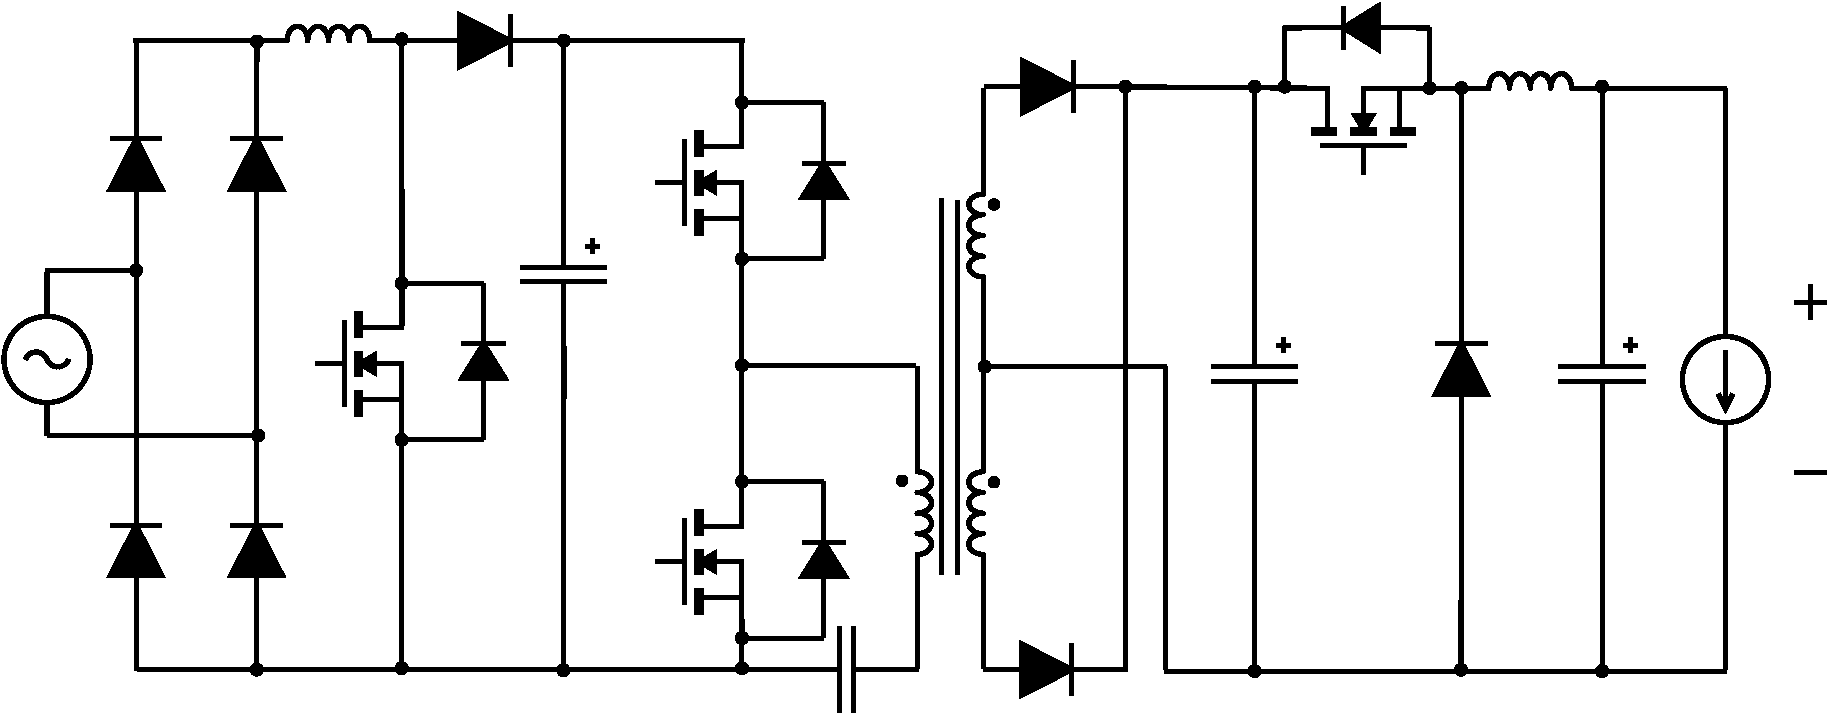
\includegraphics[width=\columnwidth]{Figures_v2/Fig1a.pdf} % Make sure this file exists
        \label{fig:1a}
        }
        \\ % This double backslash forces the next image to the line below (vertical stack)
        % (b) Middle circuit
        \subfloat[]{
        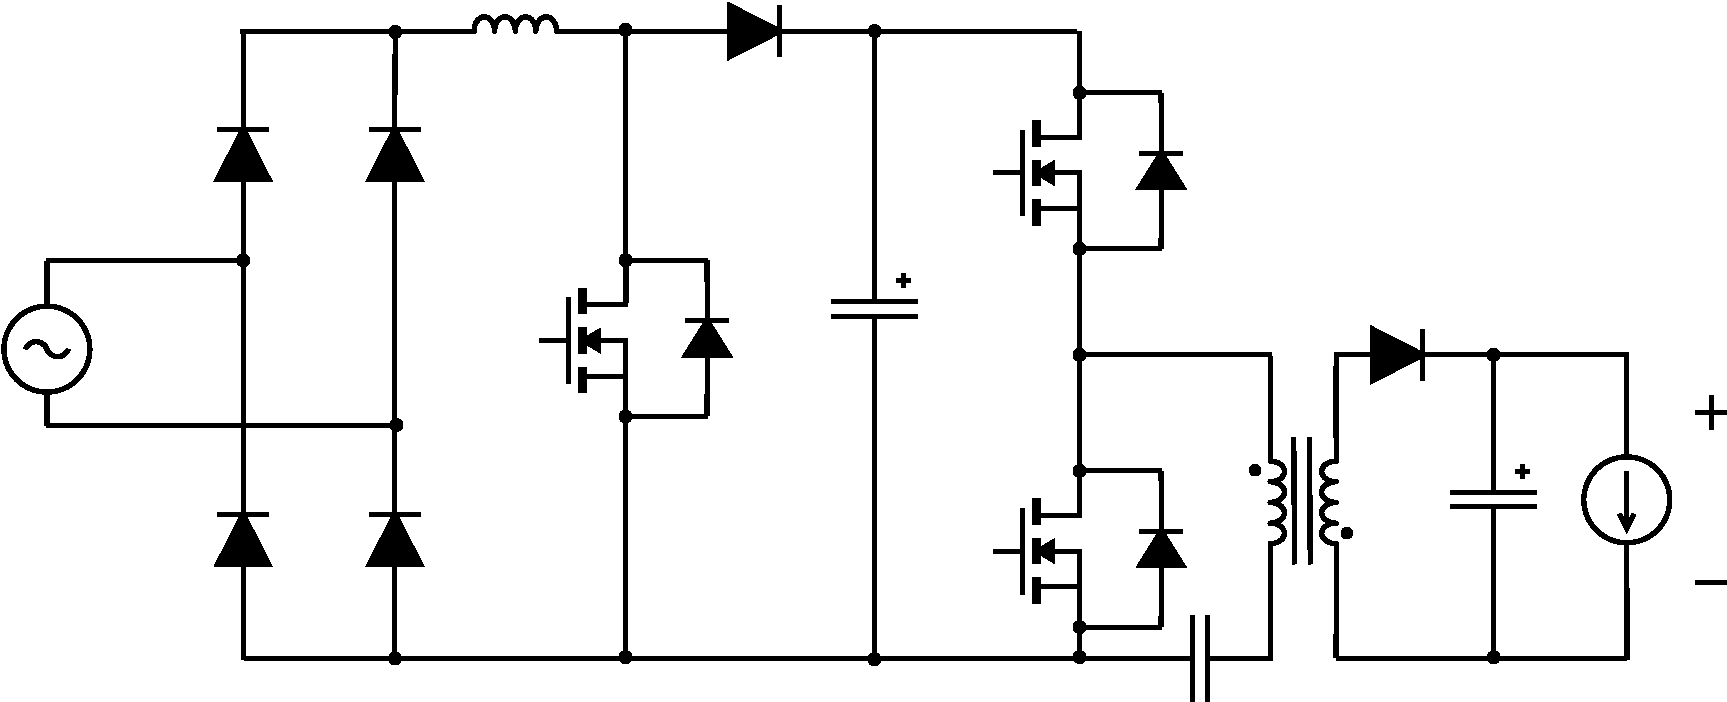
\includegraphics[width=\columnwidth]{Figures_v2/Fig1b.pdf}
        \label{fig:1b}
        }
        \\ % Line break
        % (c) Bottom circuit
        \subfloat[]{
        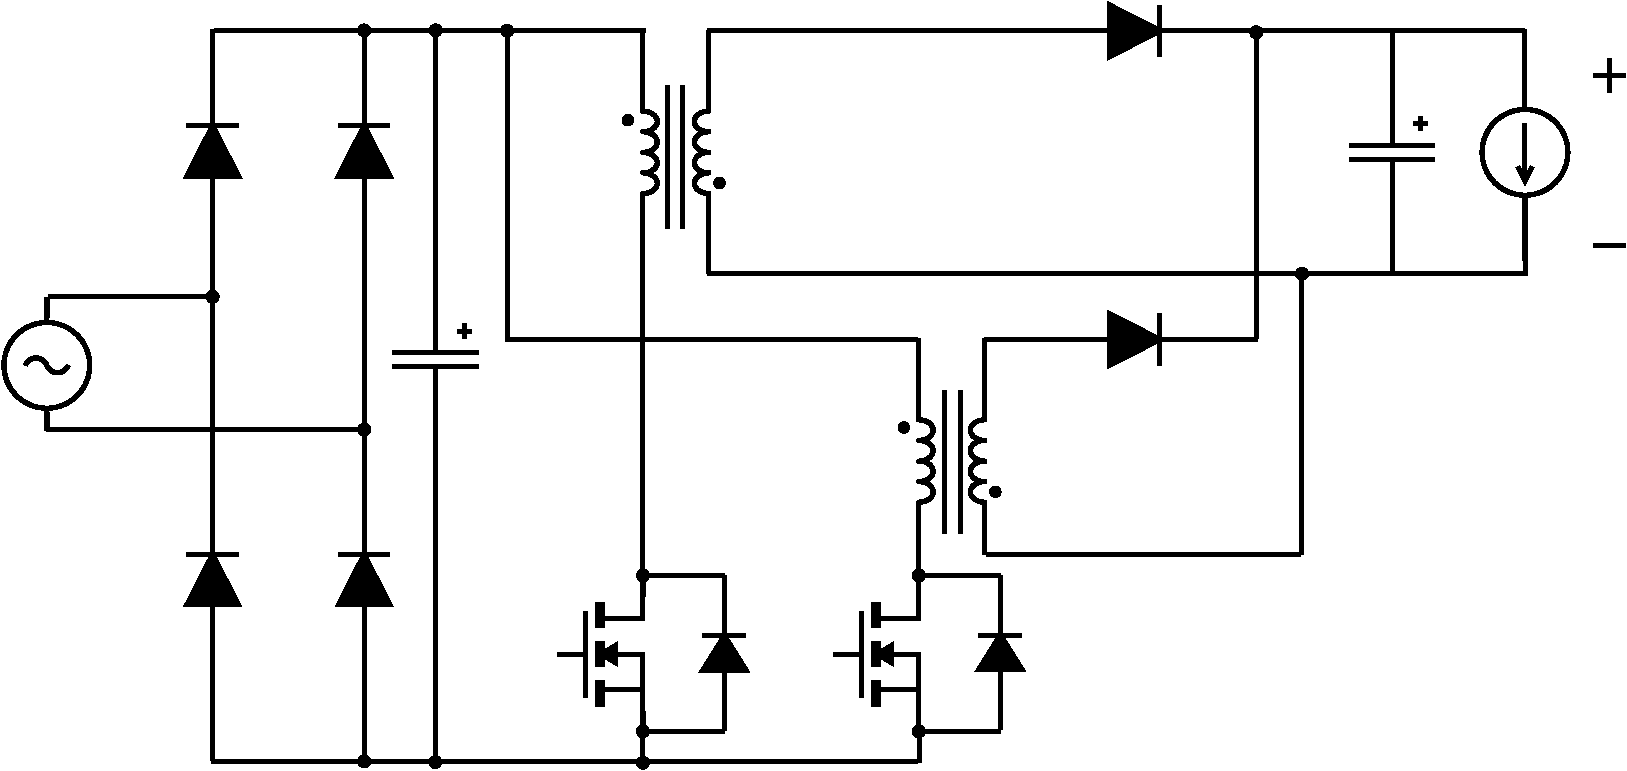
\includegraphics[width=\columnwidth]{Figures_v2/Fig1c.pdf}
        \label{fig:1c}
        }
        \caption{Power supply configurations proposed for PD applications: (a) PFC boost, LLC, and buck converter combination in \cite{ref3,ref4}, (b) PFC boost with AHB flyback \cite{ref1}, (c) two-phase interleaved flyback PFC rectifier.}
        \label{fig:configurations}
\end{figure}

Interleaving rectifiers have been considered to increase the maximum output power. Two-phase interleaving allows half of the total power to be supplied in each phase, therefore reducing the possible stress on the circuit elements \cite{ref12}. The topology is shown in Fig. \ref{fig:1c}, where the two phases are parallel in the input and output side. The source nodes of switches $S_1$ and $S_2$ are common, and only one power supply is required for gate drive circuits. A common cathode package can be used for diodes $D_1$ and $D_2$, therefore fewer components are used for the circuit. 

Operating multi-phase flyback converters across a wide output range presents some challenges. For instance, to ensure high efficiency across wide-range applications, converters must commonly employ phase-shedding, for which various control schemes have been proposed \cite{Su_2013, Zhang_2013}, \cite{Chen_2014}. This strategy deactivates specific operational phases depending on the load condition to optimize light-load efficiency. However, the implementation of these control schemes often necessitates complicated designs and additional active components, thereby increasing the circuit complexity. 

Moreover, increasing the number of phases inherently means an increase in the magnetic components required for the circuit. In the topology utilized for this study, although fewer active components are used overall, two discrete transformers are required, which compromises the power density of the converter. Integrated magnetics have been proposed and widely studied to improve the power density of various types of converters. Because integrated magnetics consolidate multiple discrete components through separate windings on a single magnetic core, these components inherently share the same flux paths, which translates to magnetic coupling. Consequently, the winding structure requires careful design to control magnetic flux. 

While magnetic coupling offers certain advantages, it introduces operational limitations. When mutual coupling exists between windings, the phases influence one another. In some coupled  topologies, utilizing phase-shedding for single-phase operation at light loads induces a voltage across the inactive phase. This generates circulating currents that degrade light-load efficiency \cite{Yang_2020, Z_Li_2025}. Even under heavy-load conditions with multiple active phases, coupling can facilitate power delivery across non-operational phase intervals, leading to input current distortion and additional induced losses, therefore reducing overall efficiency \cite{Yang_2020}. Moreover, sharing flux paths within a single core can introduce severe parasitic challenges for flybacks. The physical proximity of shared winding due to tight coupling in some integrated transformers introduces severe inter-winding stray capacitances, which can trigger high-frequency resonances and current spikes during switching transitions, and significantly increase power losses \cite{meng2021}. Some integrated planar transformers for flybacks struggle to maintain zero-voltage switching (ZVS) across wide input ranges due to the severe parasitic capacitances inherent to their multi-layer PCB structures \cite{kwon2024}. With coupling, achieving optimal operation under asymmetrical conditions must be more difficult with these added parasitics, and can thus affect reliability.

For heavy-load applications, however, magnetic coupling can be beneficial. Coupling passively forces current equalization and minimizes capacitive current ripple, while the integrated structure improves power density. This intentional coupling is utilized in fixed-load server power supplies and LLC resonant converters \cite{Ahmad}, \cite{Dou, Nakakohara}. Furthermore, modern interleaved flybacks require additional active switching devices for clamp circuits to ensure this current sharing \cite{Z_Chen_s42835}. Ultimately, while coupled magnetic structures are effective for fixed heavy-load targets, they conflict with the independent phase operation required by wide-range, variable-power converters.

Recent developments in interleaved flyback rectifiers have focused heavily on optimizing switching performance and power density. Several recent interleaved topologies still utilize discrete transformers to ensure simple control and independent operation \cite{shi2024}, \cite{cheng2018}, \cite{wu2015}, \cite{cheng2023}, \cite{mayer2025}. To offset the volumetric penalty of using discrete cores, these designs often incorporate additional auxiliary components to realize distinct operational benefits. For example, discrete multi-transformer configurations have been paired with auxiliary branches to enable active clamp soft-switching \cite{shi2024}, while other designs utilize clamping diodes or auxiliary switches to recycle transformer leakage energy \cite{cheng2018, wu2015}. Furthermore, adopting wide-bandgap GaN power devices allows these discrete configurations to operate at ultra-high switching frequencies up to 1~MHz \cite{cheng2023}. Additionally, an approach proposed in \cite{mayer2025} enables wide output voltage gain and bidirectional capability by introducing an additional coupled inductor at the output stage. While these discrete approaches effectively protect switching devices, improve conversion efficiency, and extend operational capabilities, they inherently compromise overall system power density and increase footprint by requiring multiple separate magnetic cores.

To overcome the volume limitations of discrete implementations, integrated magnetic structures for interleaved flybacks have also been researched \cite{ishihara2015},\cite{tonolo2025}, \cite{qian2008}. In these configurations, magnetic coupling is intentionally introduced to realize distinct operational benefits. For instance, intentional coupling between phases of the integrated transformer using an EE-core has been utilized to achieve reduction of ripple current \cite{ishihara2015}. Coupling between four windings of a coupled inductor was utilized to enable soft-commutation in current-fed PFC rectifiers \cite{tonolo2025}. However, these approaches require complex tuning of the coupling coefficients and design parameters. The transformer in \cite{qian2008} utilizes an EE-core with inversely coupled secondary windings to meet specific output current ripple requirements. However, the inverse coupling may introduce unwanted circulating currents or EMI if not properly managed. Therefore, the introduction of coupling can introduce some complications in manufacturing. For interleaving, coupling makes control design more complicated, as the coupling coefficients have to be taken into account in the transfer functions, since coupling causes cross talk between the phases \cite{Mao_2011}. 


Structural decoupling approaches have been explored to bypass these circulating currents and accommodate the variable-load requirements of USB PD, offering an alternative to control-based phase shedding. Some approaches design decouples phases by separating the flux paths using  3-D orthogonal-flux core geometries \cite{Ouyang},\cite{fayyaz2025}. However, these custom cores constrain commercial manufacturability and increases fabrication costs. Another proposed solution is an integrated nonlinear coupled inductor designed to decouple four phases at light loads \cite{Z_Li_2025}. Achieving this variable coupling requires customized, multi-piece L- and T-shaped core assemblies with manually configured geometries, introducing tight assembly tolerances and manufacturing complexity. To clarify the operational trade-offs among these existing approaches, a comprehensive comparison of state-of-the-art interleaved flyback topologies and their magnetic configurations is summarized in Table I.

\begin{table*}[b!]
    \caption{Comparison of State-of-the-Art Interleaved Flyback Configurations}
    \centering
    \footnotesize
    \begin{tabular}{l m{4cm} m{4.5cm} m{4.5cm}}
        \hline
        \textbf{Configuration} & \textbf{Transformer Type} & \textbf{Key Advantages} & \textbf{Drawbacks / Limitations} \\
        \hline \hline
        Conventional Interleaved & Multiple, discrete cores \cite{shi2024, cheng2018, wu2015, cheng2023, mayer2025} & Independent phase operation, simple control & High component count, low power density, and increased footprint \\
        Coupled Interleaved & Integrated (coupled) \cite{ishihara2015, tonolo2025, qian2008} & High power density, potential ripple reduction & Circulating currents that degrade light-load efficiency \cite{Yang_2020, Z_Li_2025}, higher parasitics \cite{meng2021, kwon2024}, and complex control \cite{Mao_2011} \\
        Decoupled Interleaved & Integrated (Orthogonal / Custom Core) \cite{Z_Li_2025, Ouyang, fayyaz2025} & Independent phase operation, high power density & High manufacturing complexity due to non-standard core geometry \\
        \textbf{Proposed Configuration} & \textbf{Integrated (Non-coupled)} & \textbf{Independent phase operation, high power density, uses standard commercial EE-core} & \textbf{Complex flux distribution; structural asymmetry in the windings} \\
        \hline
    \end{tabular}
    \label{tab:literature_comparison}
\end{table*}

This paper proposes a non-coupled integrated transformer for a two-phase interleaved flyback rectifier as shown in Fig. \ref{fig:2a} to address these limitations. The structure is designed to achieve zero magnetic coupling between phases, ensuring independent phase operation without magnetic interference. The proposed winding structure is shown in Fig. \ref{fig:2b} where $N_{ab}$ is the number of turns between terminals $a$ and $b$. Half of $N_{12}$ and $N_{34}$ are wound at each outer leg with opposite polarity, so as to allow for flux cancellation at the center leg. On the other hand, $N_{56}$ and $N_{78}$ are also wound with opposite polarity on the center leg, and allows for the transformer $N_{12}$ and $N_{34}$ to not operate during its operation. 

\begin{figure}[h!]
\centering
% (a) Top circuit
        \subfloat[]{
        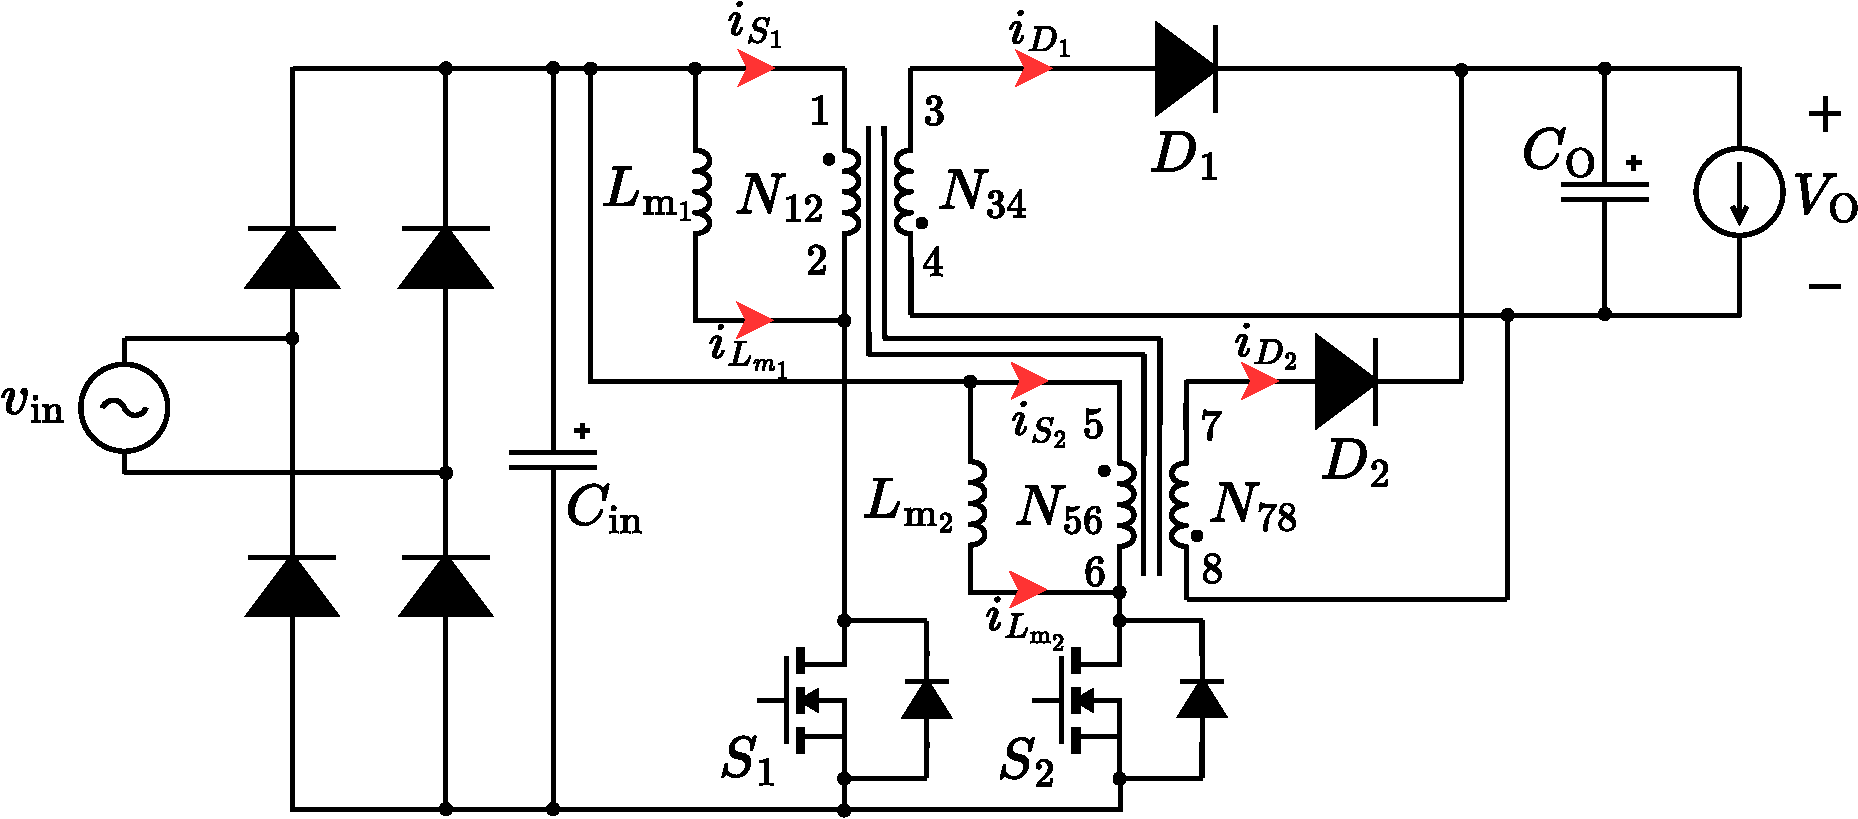
\includegraphics[width=\columnwidth]{Figures_v2/Fig2a.pdf} % Make sure this file exists
        \label{fig:2a}
        }
        \\ % This double backslash forces the next image to the line below (vertical stack)
        % (b) Middle circuit
        \subfloat[]{
        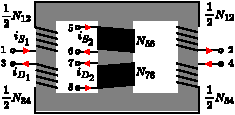
\includegraphics[width=0.6\columnwidth]{Figures_v2/Fig2b.pdf}
        \label{fig:2b}
        }
        \caption{The two-phase interleaved flyback rectifier (a), with the transformer and its winding structure in (b).}
\end{figure}

The zero-coupling coefficient between the two separate transformers simplifies implementation of rectifiers and transformer design. The operation of the rectifiers in each interleaved phase still follows that of a conventional flyback converter, preserving simplicity in control and timing. The design is also highly dependent on the duty cycle, an easily adjustable parameter in circuit design. The converter in this study aims to operate in DCM in order to allow for easier implementation of PFC and to conform to the standards of USB PD. It also realizes independent phase operation, allowing the circuit to function in one-phase mode if desired, thereby enhancing flexibility in circuit operation and allowing simple implementation of phase-shedding. Furthermore, this entirely decoupled winding structure is easily achievable using a conventional  EE-core, successfully bypassing the manufacturing complexities of custom geometries.

This article is an extended research of \cite{ECCE}. The preliminary study in \cite{ECCE} focused on the foundational design and experimental validation of the non-coupled integrated transformer. Key additions include a more detailed theoretical analysis, simulation validation of the operational principle, transformer design methodology including air-gap design, and a comprehensive core volume analysis utilizing the area product (AP) method. The rest of this paper is organized as follows: Section II presents an operational analysis of a two-phase interleaved flyback rectifier with the integrated transformer, along with its design method. Section III describes the size reduction effect of the transformer. Sections IV and V discuss the results of the simulation and experimental verification respectively, and Section VI presents the conclusions of this paper.

\section{Design Method of the Proposed Transformer}
\subsection{Operation Analysis of the Proposed Flyback Rectifier and Transformer}
The proposed integrated transformer, shown in Fig. \ref{fig:2b} was designed for a two-phase interleaved flyback PFC rectifier, shown in Fig. \ref{fig:2a} operating in discontinuous conduction mode (DCM). The switches ($S_1$, $S_2$ in Fig. \ref{fig:2a}) operate with a fixed duty cycle $D$, fixed switching frequency $f_\mathrm{s}$, and a 180-degree phase shift. The input capacitor $C_\mathrm{in}$ acts as a high-frequency filter to bypass the switching current ripple. Because it is connected directly after the bridge diode, the voltage across $C_\mathrm{in}$ inherently follows the rectified AC line voltage. Therefore, its required voltage rating must be selected to safely exceed the peak AC input voltage.

Half of $N_{12}$ and $N_{34}$ are wound at each outer leg with opposite polarity. Moreover, $N_{56}$ and $N_{78}$ are also wound with opposite polarity at the center leg. It should be noted that Fig. \ref{fig:2b} is a simplified representation of the winding structure, so that the location and direction of each winding can be easily pinpointed. The transformer utilizes an EE core with a center leg that has a cross-sectional area twice its outer leg, in accordance with manufacturing specifications. The magnetizing inductances for both transformers $N_{12}-N_{34}$ and $N_{56}-N_{78}$ were set to be equal, and are denoted as $L_{\mathrm{m}_1}$ and $L_{\mathrm{m}_2}$ respectively. The saturation magnetic flux in each separate transformer during each phase is expected to be consistent.

The operational principle of the rectifier with the proposed transformer is illustrated in Fig. \ref{fig:operation_modes}. Additionally, Fig. \ref{fig:4} presents the key waveforms of the six distinct operation modes. The operation modes are examined under six-time intervals relative to the switching period $T_\mathrm{s}$ of $S_1$. The rectifier is designed with $D \le 0.5 \frac{n V_{\mathrm{o}}}{V_{\mathrm{in}_{\mathrm{max}}}}$ with $n$ as the turns ratio, $V_{\mathrm{o}}$ as the output voltage, and $V_{\mathrm{in}_{\mathrm{max}}}$ as the peak value of the input voltage. This condition ensures the magnetizing current of one phase returns to zero before the other phase peaks. This duration is defined as the discharge time $t_{\mathrm{dis}}$ and is given in terms of circuit parameters by \eqref{eq:discharge}:

\begin{figure*}[htbp]
    \centering
    
    % --- LEFT COLUMN (Modes 1, 2, 3) ---
    \begin{minipage}{0.48\textwidth}
        \centering
        
        \subfloat[\label{fig:mode_1}]{%
            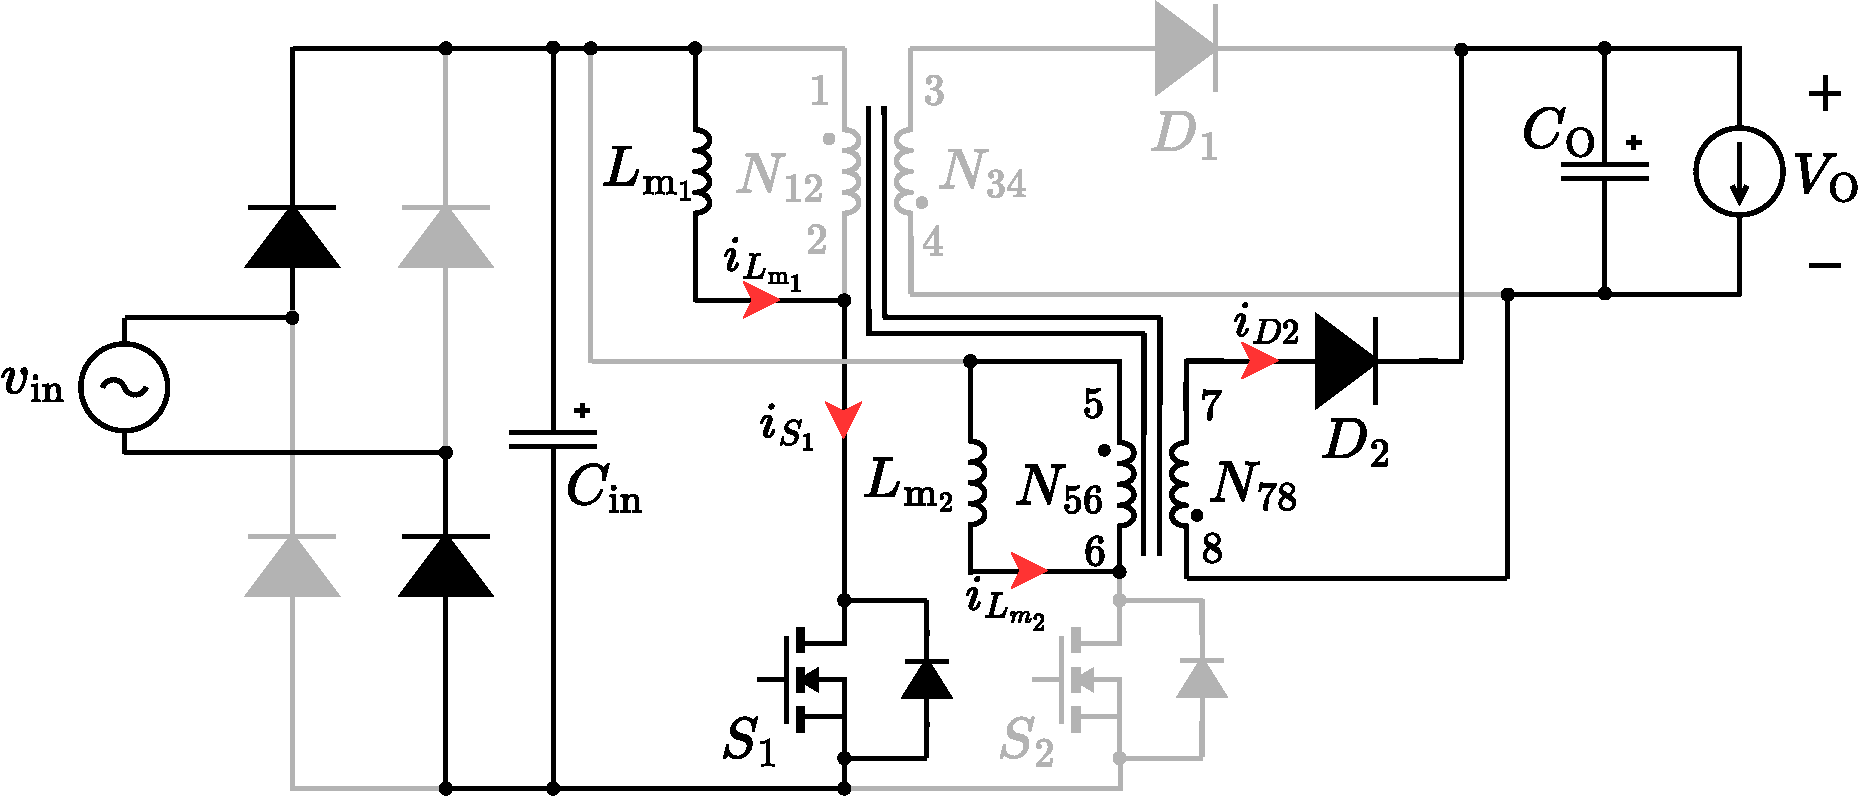
\includegraphics[width=\linewidth]{Figures_v2/Fig3a.pdf}%
        }
        
        \vspace{10pt} 
        
        \subfloat[\label{fig:mode_2}]{%
            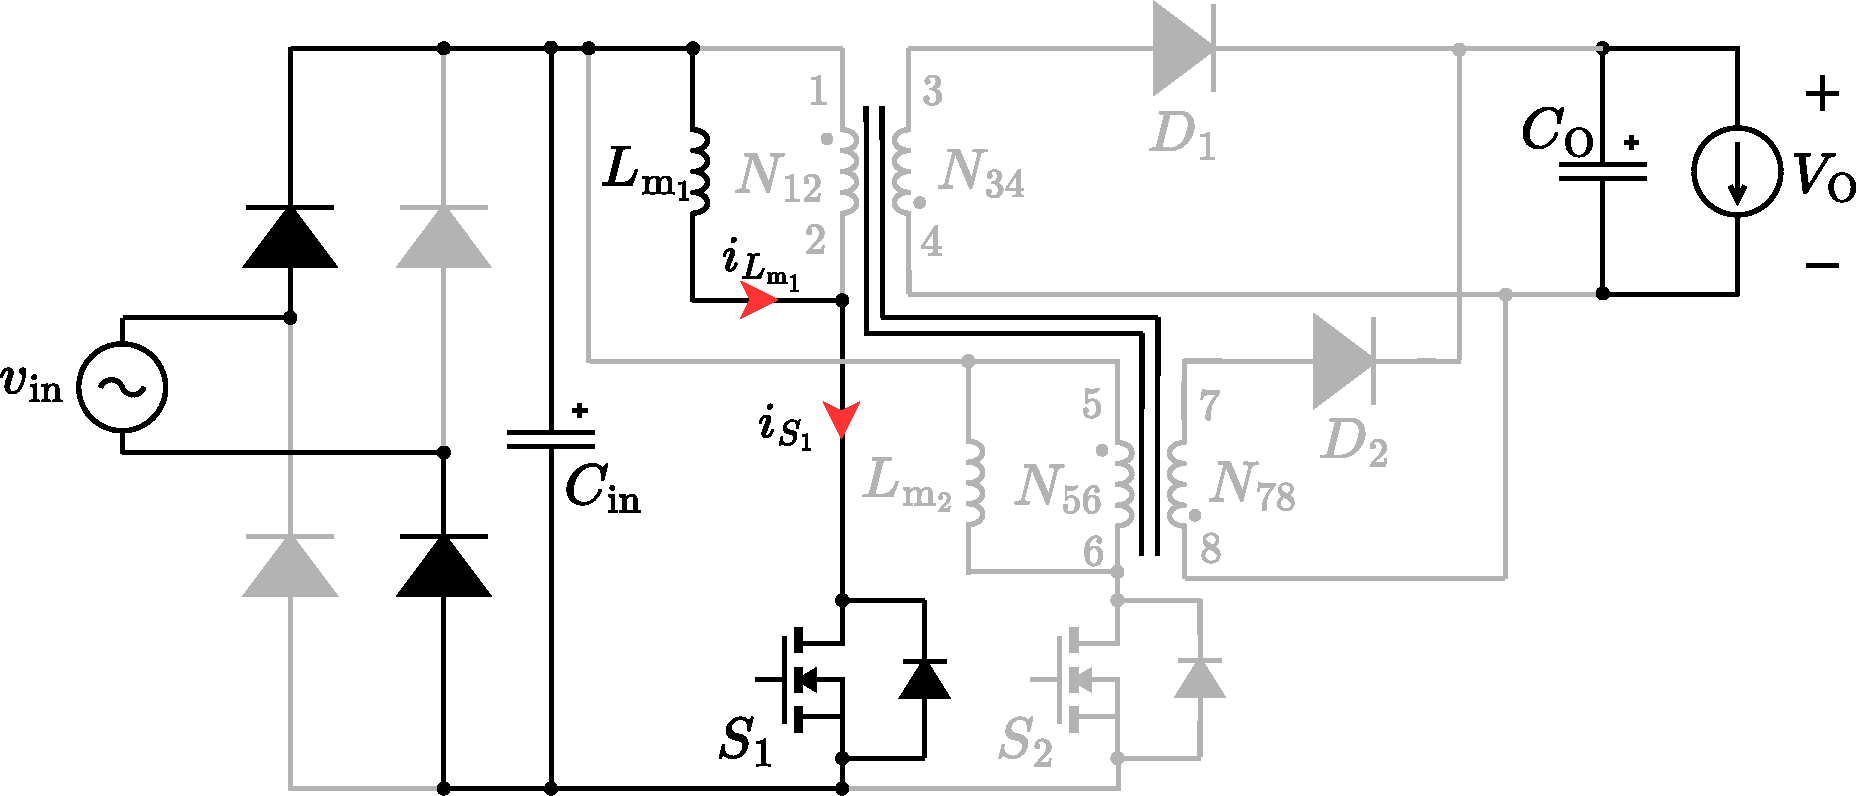
\includegraphics[width=\linewidth]{Figures_v2/Fig3b.pdf}%
        }
        
        \vspace{10pt} 
        
        \subfloat[\label{fig:mode_3}]{%
            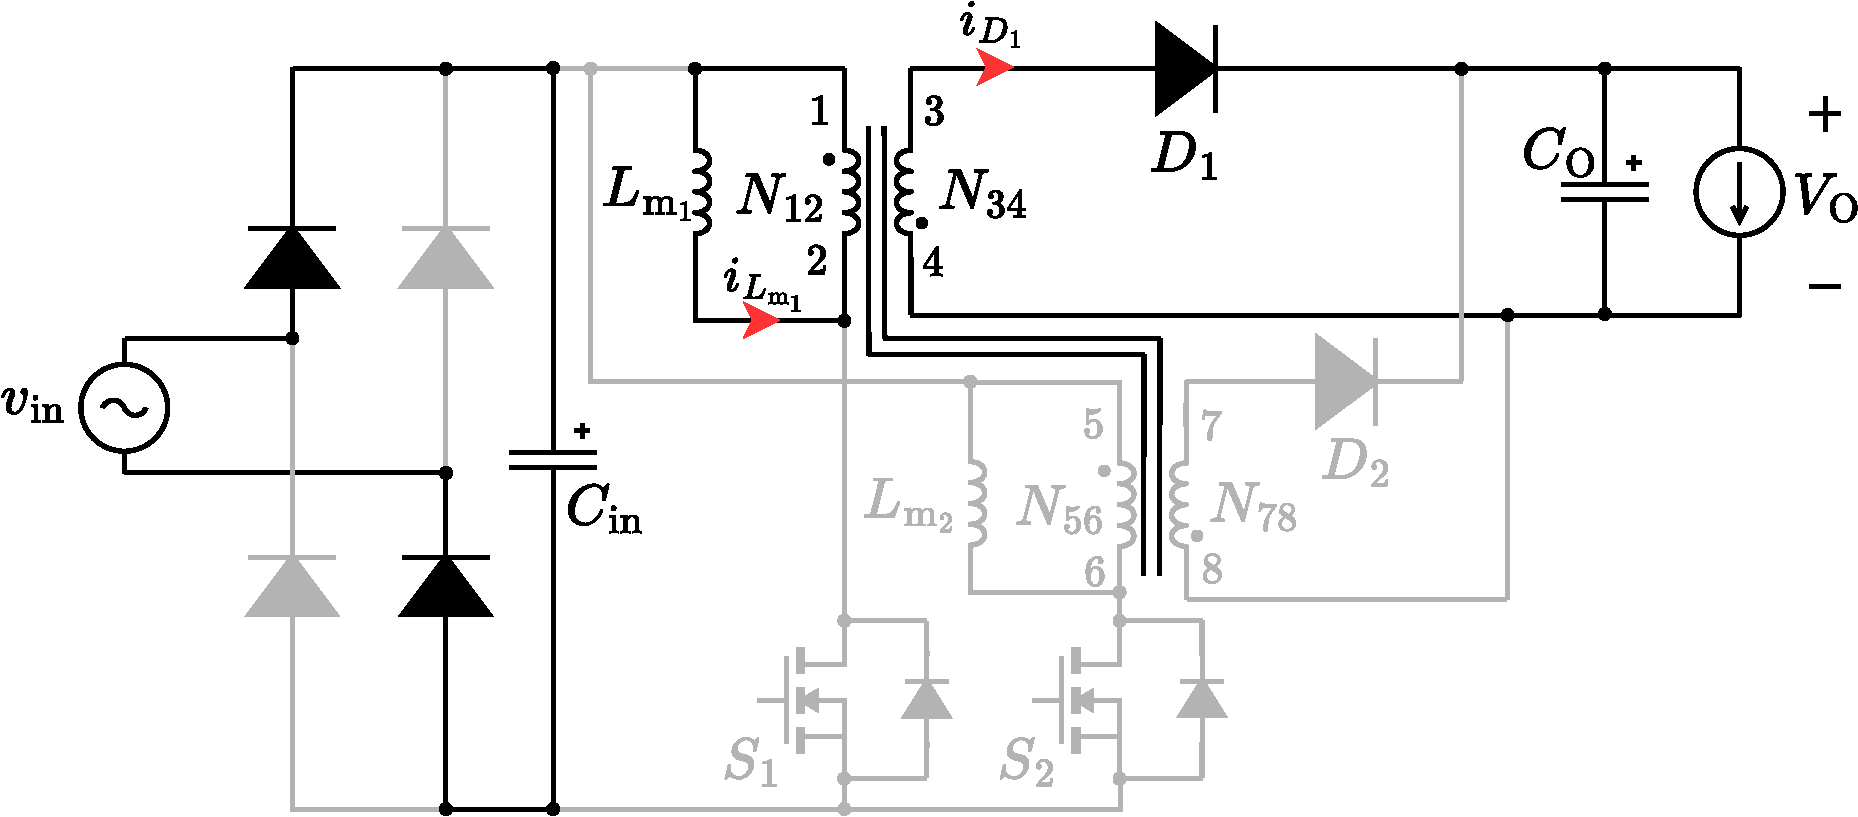
\includegraphics[width=\linewidth]{Figures_v2/Fig3c.pdf}%
        }
    \end{minipage}
    \hfill
    % --- RIGHT COLUMN (Modes 4, 5, 6) ---
    \begin{minipage}{0.48\textwidth}
        \centering
        
        \subfloat[\label{fig:mode_4}]{%
            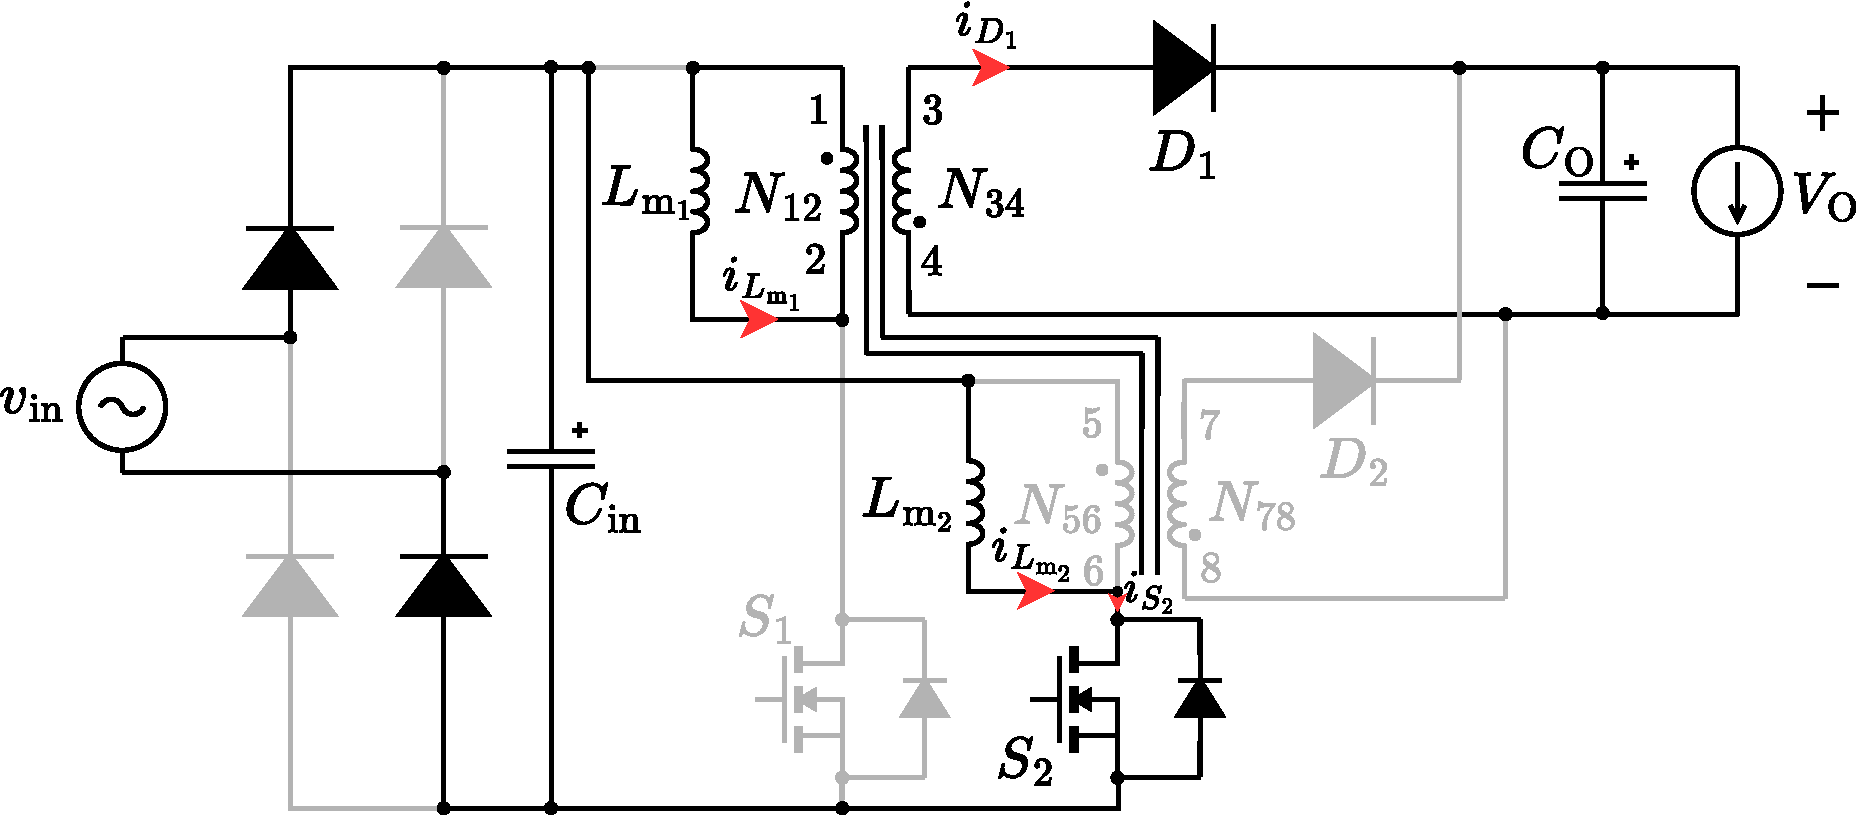
\includegraphics[width=\linewidth]{Figures_v2/Fig3d.pdf}%
        }
        
        \vspace{10pt} 
        
        \subfloat[\label{fig:mode_5}]{%
            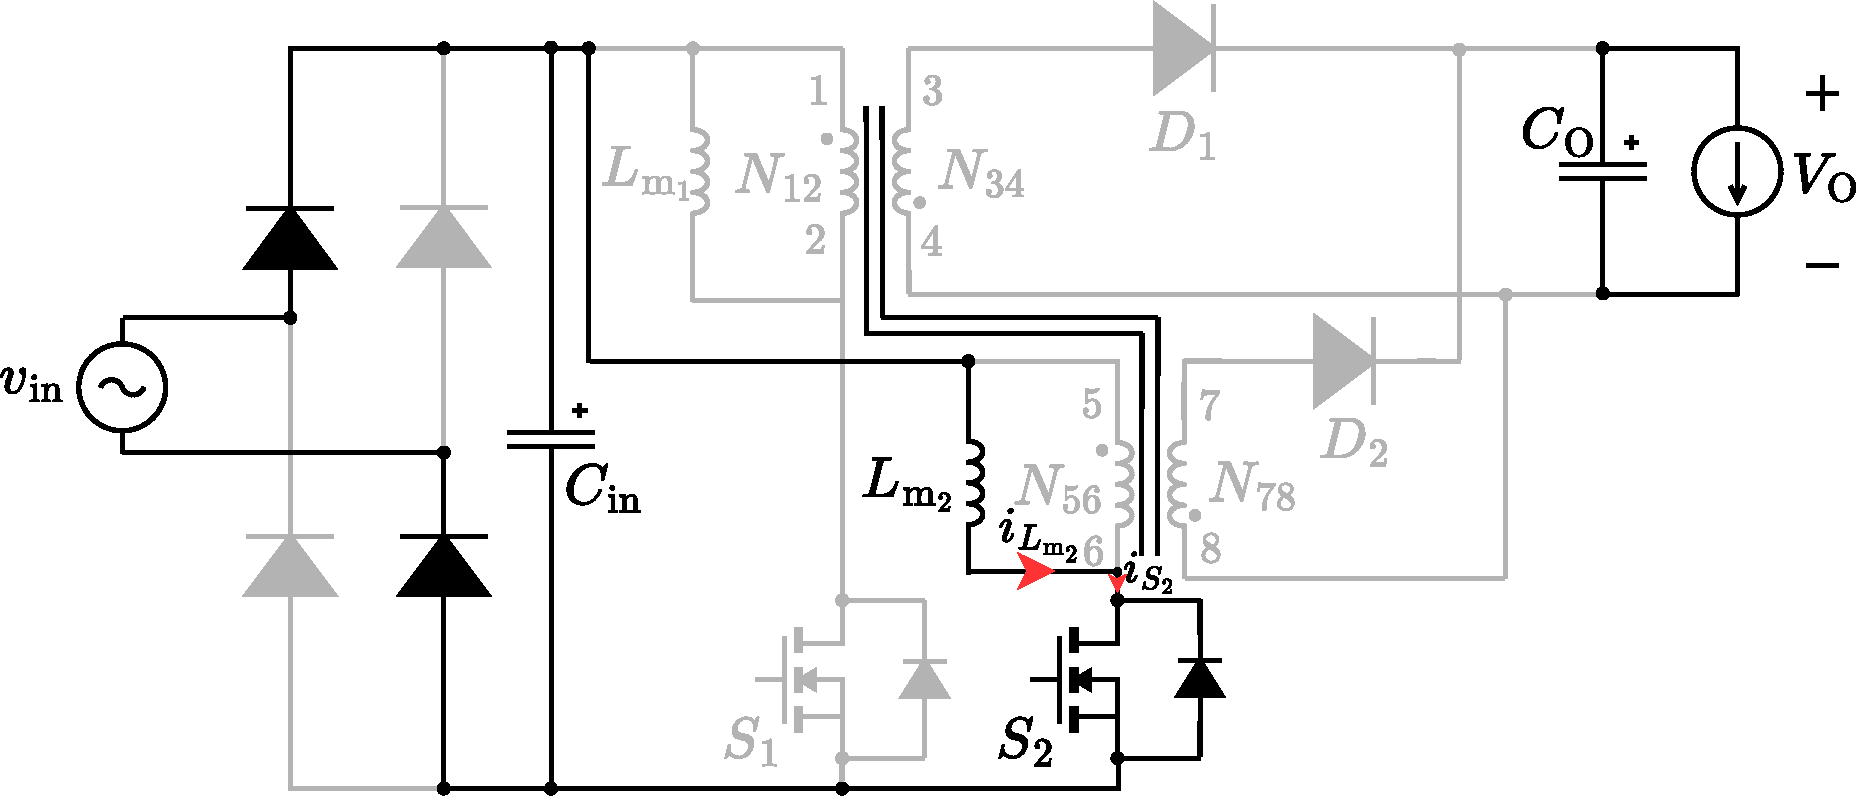
\includegraphics[width=\linewidth]{Figures_v2/Fig3e.pdf}%
        }
        
        \vspace{10pt} 
        
        \subfloat[\label{fig:mode_6}]{%
            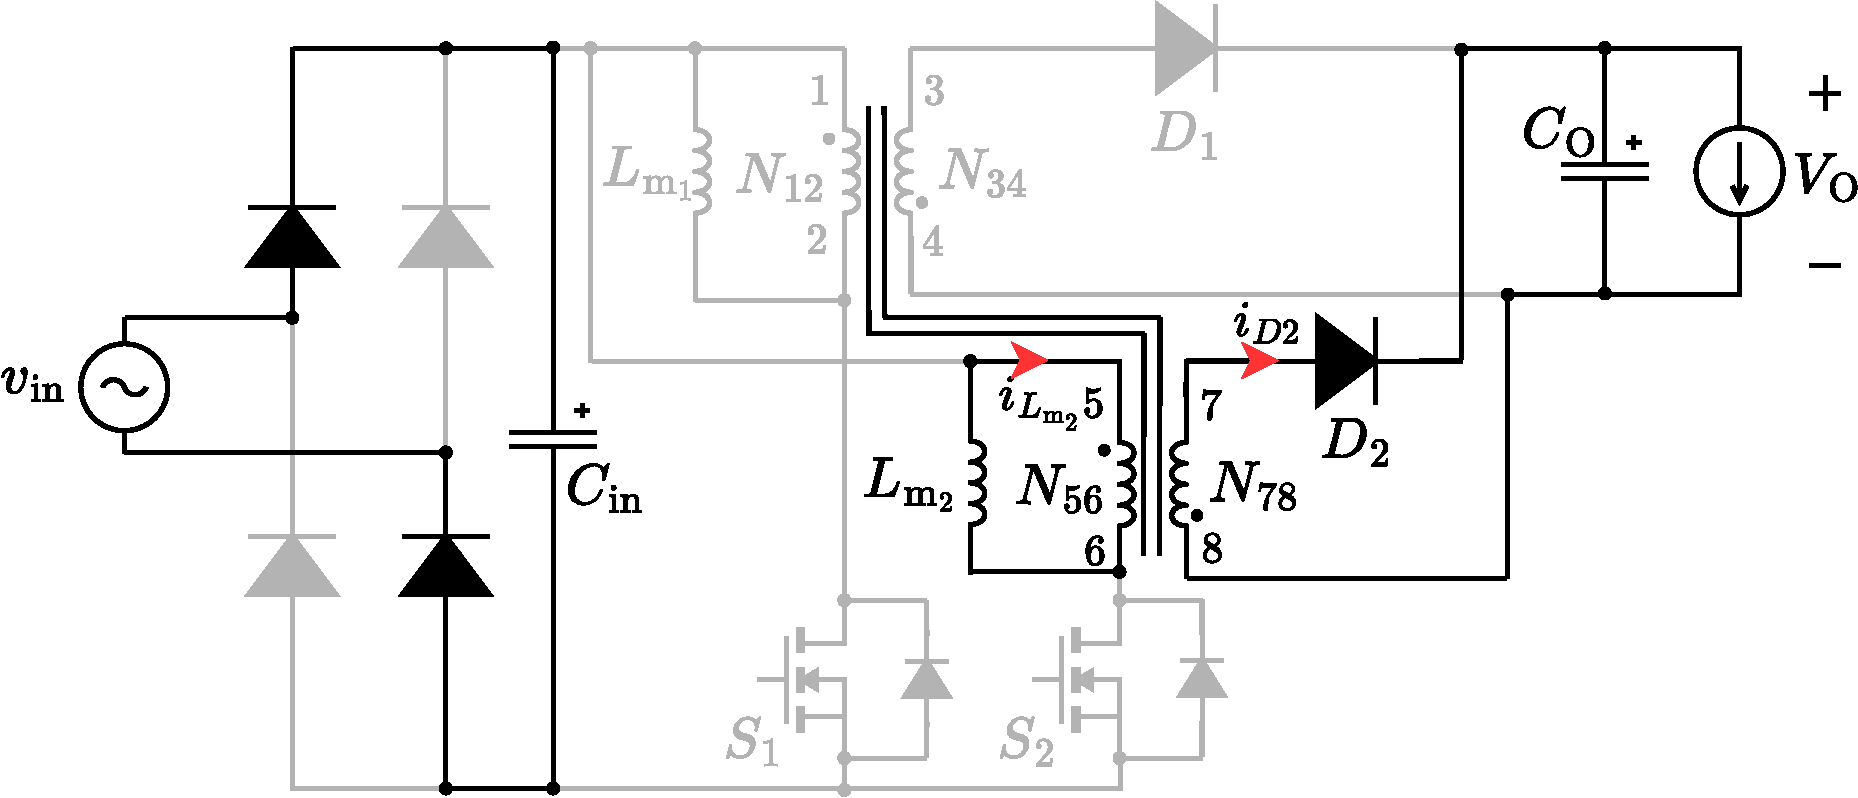
\includegraphics[width=\linewidth]{Figures_v2/Fig3f.pdf}%
        }
    \end{minipage}
    
    \caption{Operational principle of the two-phased interleaved flyback rectifier with the proposed integrated transformer at $D \le 0.5 \frac{n V_{\mathrm{o}}}{V_{\mathrm{in}_{\mathrm{max}}}}$. There are six distinct operational modes shown: (a) Mode 1 ($t_1 < t < t_2$), (b) Mode 2 ($t_2 < t < t_3$), (c) Mode 3 ($t_3 < t < t_4$), (d) Mode 4 ($t_4 < t < t_5$), (e) Mode 5 ($t_5 < t < t_6$), and (f) Mode 6 ($t_6 < t < t_7$).}
    \label{fig:operation_modes}
\end{figure*}

\begin{equation}
\label{eq:discharge}
t_{\mathrm{dis}} = \frac{V_{\mathrm{in}_{\mathrm{max}}} DT_{\mathrm{s}}}{n V_{\mathrm{o}}}
\end{equation}
with $T_{\mathrm{s}}$ as the switching period. For the condition given by $D$ in this analysis, $t_{\mathrm{dis}}$ corresponds to the interval between $t_3$ and $t_5$ in Fig. \ref{fig:4}.

\begin{figure}[htbp]
\centering
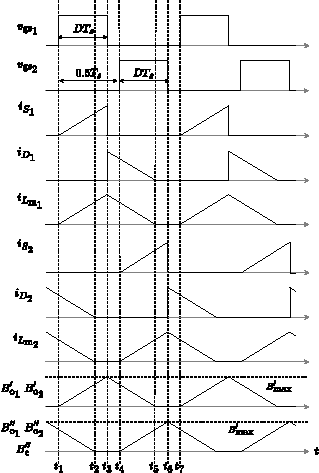
\includegraphics[width=\columnwidth]{Figures_v2/Fig4.pdf}
\caption{Key waveforms in the operation of the two-phase interleaved flyback rectifier with the proposed transformer, with $D \le 0.5 \frac{n V_{\mathrm{o}}}{V_{\mathrm{in}_{\mathrm{max}}}}$. $S_1$ and $S_2$ operate $180^\circ$ out of phase and have the same $T_{\mathrm{s}}$. The flux densities $B'$ and $B''$ represent the individual, un-superimposed magnetic flux components generated in the first and second active phase by $N_{12}-N_{34}$ and $N_{56}-N_{78}$ respectively.}
\label{fig:4}
\end{figure}

To describe the magnetic state of the core, the superposition principle is used, as shown in Fig. \ref{fig:5a}. The magnetic flux density component $B'$ is generated by the transformer active in the first phase defined as $N_{12}-N_{34}$. The magnetic flux density component $B''$ represents the component generated by the transformer active in the second phase defined as $N_{56}-N_{78}$. The total flux in the core legs is the algebraic sum of these components. This superposition determines the peak flux density required for the core design, which is analyzed in detail in Section II-B.

Modes 1, 2, and 3 in Figs. \ref{fig:mode_1}-(c) cover the operation during the first active phase, while Modes 4, 5, and 6 in Figs. \ref{fig:mode_4}-(f) describe the operation during the second active phase. For the following modes, $B'_{\mathrm{o}_1}$, $B'_{\mathrm{o}_2}$, and $B'_{\mathrm{c}}$ represent the magnetic flux densities in the respective left, right, and center legs of the core caused by $N_{12}-N_{34}$, respectively, which are shown in Fig. \ref{fig:5b}. On the other hand, $B''_{\mathrm{o}_1}$, $B''_{\mathrm{o}_2}$, and $B''_{\mathrm{c}}$ represent the magnetic flux densities in the respective left, right, and center legs of the core caused by $N_{56}-N_{78}$, respectively, which are detailed visually in Fig. \ref{fig:5c}. The flux paths in the core caused by each transformer across the operational analysis illustrated in Fig. \ref{fig:operation_modes} are illustrated in Fig. \ref{fig:6}.

\begin{figure}[t!]
\centering
        \subfloat[]{
        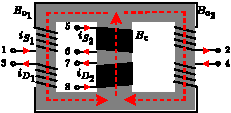
\includegraphics[width=0.6\columnwidth]{Figures_v2/Fig5a.pdf} 
        \label{fig:5a}
        }
        \\ 
        \subfloat[]{
        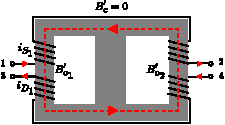
\includegraphics[width=0.6\columnwidth]{Figures_v2/Fig5b.pdf}
        \label{fig:5b}
        }
        \\
        \subfloat[]{
        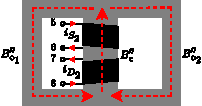
\includegraphics[width=0.53\columnwidth]{Figures_v2/Fig5c.pdf}
        \label{fig:5c}
        }
        \caption{The proposed integrated transformer during the two phases of the converter, with the flux density components in each leg illustrated in (a). (b) is the flux density contribution by $N_{12}-N_{34}$ during the first active phase, while (c) is the flux density contribution by $N_{56}-N_{78}$ during the second active phase.}
        \label{fig:5}
\end{figure}

\begin{figure*}[htbp]
    \centering
    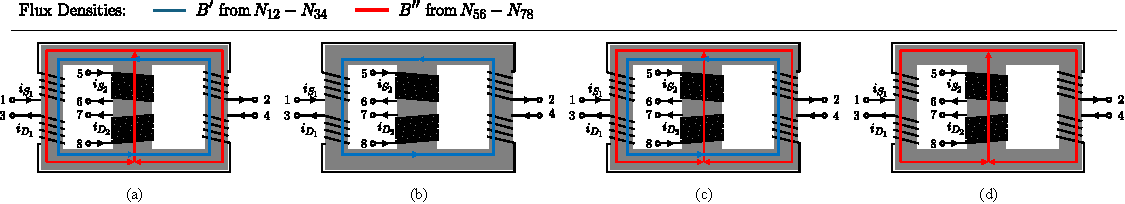
\includegraphics[width=\textwidth]{Figures_v2/Fig6new.pdf} % Change the filename if yours is different
    \caption{Magnetic flux paths in the proposed integrated transformer across the six operating modes. (a) Mode 1 ($t_1 < t < t_2$): Phase 1 is charging and Phase 2 is discharging, resulting in the coexistence of $B'$ and $B''$. (b) Modes 2 and 3 ($t_2 < t < t_4$): Phase 1 is solely active, demonstrating perfect flux cancellation in the center leg. (c) Mode 4 ($t_4 < t < t_5$): Phase 2 is charging and Phase 1 is discharging, with both $B'$ and $B''$ present. (d) Modes 5 and 6 ($t_5 < t < t_7$): Phase 2 is solely active.}
    \label{fig:6}
\end{figure*}

The detailed analysis of each operating mode is as follows:

\begin{enumerate}
    \item Mode 1 ($t_1 < t < t_2$, Fig. \ref{fig:mode_1}): At time $t_1$, switch $S_1$ turns on and $S_2$ remains off. The transformer $N_{12}-N_{34}$ begins storing energy in its magnetizing inductance. Its magnetizing current $i_{L_{\mathrm{m}_1}}$ and the corresponding flux densities in the outer legs $B'_{\mathrm{o}_1}$ and $B'_{\mathrm{o}_2}$ linearly increase from zero. Simultaneously, transformer $N_{56}-N_{78}$ completes its discharge phase, with its magnetizing current $i_{L_{\mathrm{m}_2}}$ and secondary diode current $i_{\mathrm{D}_2}$ decreasing to zero at $t_2$. During this interval, the magnetic fluxes from both transformers coexist in the core, as illustrated in Fig. \ref{fig:6}(a).

    \item Mode 2 ($t_2 < t < t_3$, Fig. \ref{fig:mode_2}): Mode 2 starts right after transformer $N_{56}-N_{78}$ completes its discharging phase, which means its associated currents $i_{\mathrm{D}_2}$, $i_{L_{\mathrm{m}_2}}$, and flux densities $B''_{\mathrm{o}_1}$, $B''_{\mathrm{o}_2}$, and $B''_{\mathrm{c}}$ are zero. Now, with $S_1$ still on, transformer $N_{12}-N_{34}$ continues storing energy until $i_{L_{\mathrm{m}_1}}$ reaches its peak value at $t_3$. 
    
    \vspace{\baselineskip}
    Because the converter operates as a PFC rectifier, the instantaneous input voltage follows a rectified sinusoidal envelope $v_{\mathrm{in}}(t) = V_{\mathrm{in}_{\mathrm{max}}} |\sin(2\pi f_{\mathrm{line}} t)|$, where $V_{\mathrm{in}_{\mathrm{max}}}$ is the peak AC line voltage and $f_{\mathrm{line}}$ is the line frequency. Assuming $v_{\mathrm{in}}(t)$ is quasi-static during a single high-frequency switching cycle, the time-variant peak primary current $i_{\mathrm{S}_{1_{\mathrm{pk}}}}(t)$ reached at the end of the ON-time of the first active phase is given by:
    \begin{equation}
    \label{eq:1}
    i_{\mathrm{S}_{1_{\mathrm{pk}}}}(t) = \frac{v_{\mathrm{in}}(t)}{L_{\mathrm{m}_1}} D T_{\mathrm{s}} 
    \end{equation}
    where $D$ is the duty cycle, $T_{\mathrm{s}}$ is the switching period, and $L_{\mathrm{m}_1}$ is the magnetizing inductance of transformer $N_{12}-N_{34}$. Consequently, the flux densities $B'_{\mathrm{o}_1}$ and $B'_{\mathrm{o}_2}$ also reach their cycle-specific peak values $B'_{\mathrm{o}_{\mathrm{pk}}}(t)$ which are given by \eqref{eq:2}:
    \begin{equation}
    \label{eq:2}
    B'_{\mathrm{o}_{\mathrm{pk}}}(t) = \frac{L_{\mathrm{m}_1} i_{\mathrm{S}_{1_{\mathrm{pk}}}}(t)}{N_{12} A_{\mathrm{o}}} 
    \end{equation}
    with $N_{12}$ as the number of turns in the primary side of the active transformer and $A_{\mathrm{o}}$ is the cross-sectional area of the outer leg, where the transformer $N_{12}-N_{34}$ is wound.

    \item Mode 3 ($t_3 < t < t_4$, Fig. \ref{fig:mode_3}): Mode 3 starts right after transformer $N_{12}-N_{34}$ finishes charging. At $t_3$, Switch $S_1$ turns off, initiating the discharge phase of transformer $N_{12}-N_{34}$. The magnetizing current $i_{L_{\mathrm{m}_1}}$, diode current $i_{\mathrm{D}_1}$, and flux densities $B'_{\mathrm{o}_1}$ and $B'_{\mathrm{o}_2}$ begin to decrease linearly. Transformer $N_{56}-N_{78}$ remains inactive in this period.
\end{enumerate}
\vspace{\baselineskip}
Transformer $N_{12}-N_{34}$ operates as follows. The magnetomotive force and magnetic resistance of both outer legs for $N_{12}-N_{34}$ are equal. This causes the magnetic flux from the outer legs that flow into the center leg to be canceled. This causes no electromotive force generated in transformer $N_{56}-N_{78}$. As illustrated in Fig. \ref{fig:6}(b), during Modes 2 and 3, the flux solely flows on the outer legs. Therefore, the transformer formed by the outer legs operates independently from the transformer in the center leg. The equivalent magnetic circuit for this transformer is shown in Fig. \ref{fig:7}(a).
\vspace{\baselineskip}
\begin{enumerate}
    \setcounter{enumi}{3}
    \item Mode 4 ($t_4 < t < t_5$, Fig. \ref{fig:mode_4}): Mode 4 operates similarly to the positive cycle. Switch $S_2$ turns on at $t_4$ and $S_1$ remains off. Transformer $N_{56}-N_{78}$ stores energy in its magnetizing inductance. Its current $i_{L_{\mathrm{m}_2}}$ and the corresponding flux densities $B''_{\mathrm{o}_1}$, $B''_{\mathrm{c}}$ and $B''_{\mathrm{o}_2}$ linearly increase. Simultaneously, transformer $N_{12}-N_{34}$ completes its discharge phase, with $i_{L_{\mathrm{m}_1}}$ and $i_{\mathrm{D}_1}$ decreasing to zero at $t_5$. Similar to Mode 1,  $B'$ and $B''$ coexist, as shown in Fig. \ref{fig:6}(c).

    \item Mode 5 ($t_5 < t < t_6$, Fig. \ref{fig:mode_5}): Mode 5 starts after the discharge of transformer $N_{12}-N_{34}$ completes. Now, with Switch $S_2$ still on, transformer $N_{56}-N_{78}$ continues storing energy until $i_{L_{\mathrm{m}_2}}$ reaches its peak value at $t_6$. Similarly bounded by the input voltage envelope, the time-variant peak primary current $i_{\mathrm{S}_{2_{\mathrm{pk}}}}(t)$ reached at the end of the ON-time of the second active phase is given by:
    \begin{equation}
    \label{eq:3}
    i_{\mathrm{S}_{2_{\mathrm{pk}}}}(t) = \frac{v_{\mathrm{in}}(t)}{L_{\mathrm{m}_2}} D T_{\mathrm{s}} 
    \end{equation}
    where $L_{\mathrm{m}_2}$ is the magnetizing inductance of transformer $N_{56}-N_{78}$. Consequently, the flux densities $B''_{\mathrm{o}_1}$, $B''_{\mathrm{c}}$ and $B''_{\mathrm{o}_2}$ also reach their cycle-specific peak values. The time-variant peak value of the center leg flux density $B''_{\mathrm{c}_{\mathrm{pk}}}(t)$ is given by \eqref{eq:4}:
    \begin{equation}
    \label{eq:4}
    B''_{\mathrm{c}_{\mathrm{pk}}}(t) = B''_{\mathrm{o}_{\mathrm{pk}}}(t) = \frac{L_{\mathrm{m}_2} i_{\mathrm{S}_{2_{\mathrm{pk}}}}(t)}{N_{56} A_{\mathrm{c}}} 
    \end{equation}
    with $N_{56}$ as the number of turns in the primary side of the active transformer and $A_{\mathrm{c}}$ is the cross-sectional area of the center leg where the transformer $N_{56}-N_{78}$ is wound.

    \item Mode 6 ($t_6 < t < t_7$, Fig. \ref{fig:mode_6}): Switch $S_2$ turns off, initiating the discharge phase of transformer $N_{56}-N_{78}$. The currents $i_{L_{\mathrm{m}_2}}, i_{\mathrm{D}_2},$ and flux densities $B''_{\mathrm{o}_1}$, $B''_{\mathrm{c}}$, and $B''_{\mathrm{o}_2}$ begin to decrease linearly. Transformer $N_{12}-N_{34}$ remains inactive.
\end{enumerate}

\vspace{\baselineskip}

Transformer $N_{56}-N_{78}$ operates as follows. The magnetic resistance of both outer legs is equal, causing the magnetic flux from the center legs to be divided equally into both outer legs. Since the number of turns of both outer legs is equal and wound in an opposite polarity, the electromotive force generated in $N_{12}-N_{34}$ is canceled. As illustrated in Fig. \ref{fig:6}(d), during Modes 5 and 6, only the flux from the center legs flows through the transformer. Therefore, the transformer formed by the center leg operates independently from the transformer in the outer leg, and the equivalent magnetic circuit for this case is shown in Fig. \ref{fig:7}(b).

% -------- MAGNETIC CIRCUIT FIGURE GOES HERE --------
\begin{figure}[b!]
\centering
        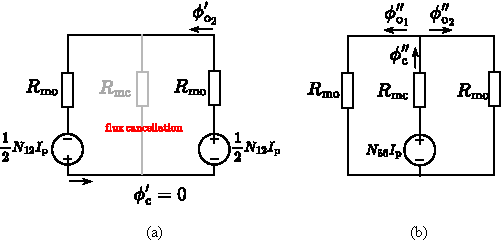
\includegraphics[width=0.92\columnwidth]{Figures_v2/Fig6.pdf} % Change filename if needed
      \caption{Equivalent magnetic circuits for the proposed transformer. (a) shows the equivalent magnetic circuit for $N_{12}-N_{34}$, while (b) shows the equivalent magnetic circuit for $N_{56}-N_{78}$.}
      \label{fig:7}
\end{figure}
% ---------------------------------------------------

As derived in the expanded time-variant equations for Mode 2 and Mode 5, the linear switching ramps are continuously bounded by the low-frequency cycle of $v_{\mathrm{in}}$. Consequently, both the instantaneous switch current stress and the peak core flux density vary dynamically across the line period. The converter components experience their absolute maximum operational stresses exclusively at the peak of the AC line voltage $V_{\mathrm{in}_{\mathrm{max}}}$.

The proposed winding structure achieves zero magnetic coupling between the two transformers. Consequently, the distinct magnetic circuits share a single core without magnetic interference. Each transformer maintains independent operation despite the physical integration. This structure eliminates the need for two discrete magnetic components. As a result, the total volume of the magnetic components is significantly reduced.

Because the proposed integrated transformer achieves magnetic decoupling, the fundamental DCM operation of the converter remains electrically identical to a conventional interleaved topology utilizing discrete transformers. As a result, the standard electrical benefits of two-phase interleaving are fully preserved.

Furthermore, operating the rectifier in DCM with a fixed $f_{\mathrm{s}}$ and constant $D$, inherently achieves PFC because the average input current $\langle i_{\mathrm{in}}(t) \rangle$ tracks the $v_{\mathrm{in}}(t)$. This inherent behavior is derived as follows.

Using \eqref{eq:1}, the average input current $\langle i_\mathrm{S_1}(t) \rangle$ for the first phase over one $T_\mathrm{s}$ is given by \eqref{eq:ave}:
\begin{align}
    \label{eq:ave}
\langle i_\mathrm{S_1}(t) \rangle &= \frac{1}{T_\mathrm{s}}\int_{0}^{T_\mathrm{s}}i_\mathrm{S_1}(\tau)d\tau \nonumber \\ &= \frac{1}{2} i_{\mathrm{S}_{1_{\mathrm{pk}}}}(t) D = \frac{v_{\mathrm{in}}(t) D^2 T_{\mathrm{s}}}{2 L_{\mathrm{m}_1}} 
\end{align}

Because the interleaved phases are symmetrical and share the same magnetizing inductance with $L_{\mathrm{m}_1} = L_{\mathrm{m}_2} = L_{\mathrm{m}}$, the second phase draws an identical average current $\langle i_{\mathrm{S}_2}(t) \rangle$. The total average input current $\langle i_{\mathrm{in}}(t) \rangle$, is the sum of both active phases:
\begin{equation}
\langle i_{\mathrm{in}}(t) \rangle = \langle i_{\mathrm{S}_1}(t) \rangle + \langle i_{\mathrm{S}_2}(t) \rangle = \frac{D^2 T_{\mathrm{s}}}{L_{\mathrm{m}}} v_{\mathrm{in}}(t)
\end{equation}

Since $D$, $L_{\mathrm{m}}$, and $f_{\mathrm{s}}$ are constant, $\langle i_{\mathrm{in}}(t) \rangle$ is directly proportional to $v_{\mathrm{in}}(t)$. Consequently, $ i_{\mathrm{in}}(t)$ inherently tracks the AC envelope, thus naturally achieving PFC. Because this fundamental electrical behavior remains identical to a standard interleaved topology operating in DCM, both the PFC and Total Harmonic Distortion (THD) performance are expected to match that of a conventional discrete setup.

\subsection{Saturation Magnetic Flux Density Analysis}
\begin{figure*}[t!]
    \centering
    % The figure spans two columns, so we use figure*
    % --- (a) Case 1 ---
    % \subfloat[] automatically generates the "(a)" label. 
    % We leave the bracket empty [] because the text "Case 1" is in the main caption, not the sub-label.
    \subfloat[\label{fig:case1}]{%
        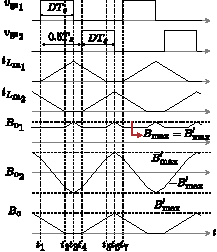
\includegraphics[width=0.32\textwidth]{Figures_v2/Fig7a.pdf}%
    }
    \hfill % Adds flexible space between images
    % --- (b) Case 2 ---
    \subfloat[\label{fig:case2}]{%
        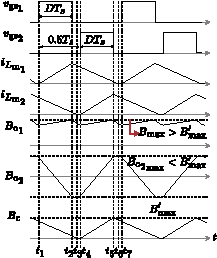
\includegraphics[width=0.32\textwidth]{Figures_v2/Fig7b.pdf}%
    }
    \hfill
    % --- (c) Case 3 ---
    \subfloat[\label{fig:case3}]{%
        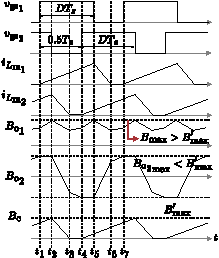
\includegraphics[width=0.32\textwidth]{Figures_v2/Fig7c.pdf}%
    }
    \caption{Theoretical, superimposed magnetic flux density waveforms in the integrated transformer during circuit operations: (a) Case 1, (b) Case 2, and (c) Case 3.}
    \label{fig:flux_waveforms}
\end{figure*}


The circuit operation is classified into three patterns determined by $D$ and the boundary condition $D \le 0.5 \frac{n V_{\mathrm{o}}}{V_{\mathrm{in}_{\mathrm{max}}}}$. This classification, illustrated in Fig. \ref{fig:flux_waveforms}, arises because the integrated single-core structure permits simultaneous magnetizing current flow in multiple active windings, resulting in distinct flux superposition compared to conventional discrete transformers. The manner of superposition due to the magnetizing current can be controlled by $t_{\mathrm{dis}}$. Consequently, the saturation magnetic flux density $B_{\mathrm{max}}$ is a critical parameter for the transformer geometry. It can be expressed in terms of the saturation magnetic flux density in each phase, denoted as $B'_{\mathrm{max}}$ and $B''_{\mathrm{max}}$, with $B'_{\mathrm{max}} = B''_{\mathrm{max}}$ since $L_{\mathrm{m}_1} = L_{\mathrm{m}_2}$. The flux density in each leg is examined further using the principle of superposition, with the expressions of the superimposed flux densities in the left, right and center legs shown in \eqref{eq:5}-\eqref{eq:7}, represented as $B_{\mathrm{o}_1}$, $B_{\mathrm{o}_2}$ and $B_{\mathrm{c}}$ respectively:
\begin{align}
B_{\mathrm{o}_1} &= B'_{\mathrm{o}_1} + B''_{\mathrm{o}_1} \label{eq:5}\\
B_{\mathrm{o}_2} &= B'_{\mathrm{o}_2} - B''_{\mathrm{o}_2} \label{eq:6}\\
B_{\mathrm{c}} &= B''_{\mathrm{c}} \label{eq:7}
\end{align}

\subsubsection*{\textup{Case 1 (Fig. \ref{fig:case1}),  $D \le 0.5 \frac{n V_{\mathrm{o}}}{V_{\mathrm{in}_{\mathrm{max}}}}$}}
The waveforms in Fig. \ref{fig:4} represent the circuit operation for Case 1. As shown, flux cancellation does not occur in the outer legs; however, the magnitude of the peak flux density remains uniform across all legs. If the magnetizing current of one phase reaches zero before the magnetizing current of the other phase reaches its peak, then $B_{\mathrm{max}} =  B'_{\mathrm{max}}$. This condition is satisfied when $D$ is expressed by \eqref{eq:8}.
\begin{equation}
\label{eq:8}
D \le 0.5 \frac{n V_{\mathrm{o}}}{V_{\mathrm{in}_{\mathrm{max}}}}
\end{equation}

\subsubsection*{\textup{Case 2 (Fig. \ref{fig:case2}), $0.5 \frac{n V_{\mathrm{o}}}{V_{\mathrm{in}_{\mathrm{max}}}} < D \le 0.5$}}
In this case, the magnetizing current of one phase does not reach zero before the subsequent phase reaches its peak. The saturation flux density across all phases can be derived as follows. At $t_2$, $B'_{\mathrm{o}_1} = B'_{\mathrm{max}}$. Moreover, $B''_{\mathrm{o}_1}(t_2) = B'_{\mathrm{o}_1}(t_5)$ and is expressed in \eqref{eq:9}:
\begin{equation}
\label{eq:9}
B''_{\mathrm{o}_1}(t_2) = B'_{\mathrm{o}_1}(t_5) = B'_{\mathrm{max}} - \frac{B'_{\mathrm{max}}}{t_6 - t_2}(t_5 - t_2)
\end{equation}
with $t_5 = 0.5 T_{\mathrm{s}} + t_2$ and $t_2 = D T_{\mathrm{s}}$. The peak $i_{L_{\mathrm{m}_{1_{\mathrm{pk}}}}}$ can be rewritten as in \eqref{eq:10}:
\begin{equation}
\label{eq:10}
i_{L_{{{\mathrm{m}_1}_{\mathrm{pk}}}}} = \frac{V_{\mathrm{in}_{\mathrm{max}}}}{L_{\mathrm{m}}} D T_{\mathrm{s}} = \frac{n V_{\mathrm{o}}}{L_{\mathrm{m}}}(t_6 - t_2)
\end{equation}

In this case, \eqref{eq:8} is not satisfied, and this results in $B_{\mathrm{max}}$ in the left outer leg exceeding $B'_{\mathrm{max}}$ in the center leg, as expressed in \eqref{eq:11}:
\begin{equation}
\label{eq:11}
B_{\mathrm{max}} = \left(2 - \frac{0.5 n V_{\mathrm{o}}}{V_{\mathrm{in}_{\mathrm{max}}} D}\right) B'_{\mathrm{max}}
\end{equation}

\subsubsection*{\textup{Case 3 (Fig. \ref{fig:case3}), $0.5 < D$}}
In this case, $B_{\mathrm{max}}$ in the left outer leg consistently exceeds $B'_{\mathrm{max}}$. By analysis similar to Case 2, $B_{\mathrm{max}}$ is derived as \eqref{eq:12}:
\begin{equation}
\label{eq:12}
B_{\mathrm{max}} = \left(1 + \frac{D - 0.5}{D}\right) B'_{\mathrm{max}}
\end{equation}

Because the flyback is interleaved, it is expected that the rectifier will primarily operate at $D \le 0.5$, which operates in the conditions set by Case 1 or 2.

\subsection{Worst-Case Operating Conditions}
To properly evaluate the converter and size the components across the universal input range ($v_{\text{in}}$ of $100\text{ V}_{\text{rms}}$ to $240\text{ V}_{\text{rms}}$), it is critical to identify the worst-case operating conditions. For both the switch current and the magnetic core, the lowest $V_{\text{in}}$ of $100\text{ V}_{\text{rms}}$ represents the practical worst-case scenario, whereas the highest $v_{\text{in}}$ of $240\text{ V}_{\text{rms}}$ dictates the worst-case switch voltage stress $v_{\text{ds}}$.

This distinction is fundamentally driven by the necessary duty-cycle adjustment. In a two-phase interleaved flyback PFC rectifier operating in DCM and delivering constant output power $P_{\text{O}}$, the duty cycle $D$ is inversely proportional to $v_{\text{in}}$, which directly follows from \cite{ref8} and is expressed in \eqref{eq:27}:

The duty cycle is calculated using \eqref{eq:27} \cite{ref8}.
\begin{equation}
\label{eq:27}
D = \frac{2}{V_{\mathrm{in}_{\mathrm{pk}}}} \sqrt{\frac{0.5 L_{\mathrm{m}} P_{\mathrm{o}}}{T_{\mathrm{s}}}}
\end{equation}

From \eqref{eq:1} and \eqref{eq:3}, using \eqref{eq:27}, the absolute peak switch currents $i_{\mathrm{S}_{pk_1(\max)}}$ and $i_{\mathrm{S}_{pk_2(\max)}}$, which are at the peak of the AC line voltage cycle, remain constant across the entire input range. It also follows from \eqref{eq:2} and \eqref{eq:4} that the absolute peak magnetic flux densities $B'_{\mathrm{o}_{1_{pk}(\max)}}$, $B'_{\mathrm{o}_{2_{pk}(\max)}}$, and $B''_{\mathrm{c}_{pk(\max)}}$ remain constant across the entire $v_{\text{in}}$ range of $100\text{ V}_{\text{rms}}$ to $240\text{ V}_{\text{rms}}$. However, while the peaks remain constant, $D$ reaches its absolute maximum at the lowest $v_{\text{in}}$. Consequently, the RMS currents in the switches and transformer windings are maximized at the lowest $v_{\text{in}}$. Furthermore, accounting for the degradation of converter efficiency at lower line voltages, the system must draw greater input power to sustain the nominal $P_{\text{O}}$. This requirement inherently elevates the actual peak currents at a $V_{\text{in}}$ of $100\text{ V}_{\text{rms}}$, establishing it as the most severe operating condition for both current stress and magnetic core saturation.

\subsection{Design Method of the Proposed Integrated Transformer}
A turns ratio $n$ is selected based on the maximum voltage ratings of the switches. The maximum operating duty cycle $D$ is selected in consideration of the desired operation discussed in Section II-B. The magnetizing inductance, $L_{\mathrm{m}_1}=L_{\mathrm{m}_2}=L_{\mathrm{m}}$ is calculated from the circuit specifications. The saturation magnetic flux density per phase $B'_{\mathrm{max}}$ is calculated from the $B_{\mathrm{max}}$ given by the chosen core material, considering the maximum $D$. A core is chosen using the AP method. 

The number of turns is calculated using $B'_{\mathrm{max}}$ and the peak primary side current $I_{\mathrm{pri}_{\mathrm{pk}}}$ as shown in \eqref{eq:13} and \eqref{eq:14}:
\begin{equation}
\label{eq:13}
\frac{N_{12}}{n} = N_{34} \ge \frac{L_{\mathrm{m}} I_{\mathrm{pri}_{\mathrm{pk}}}}{n A_{\mathrm{mo}} B'_{\mathrm{max}}}
\end{equation}
\begin{equation}
\label{eq:14}
\frac{N_{56}}{n} = N_{78} \ge \frac{L_{\mathrm{m}} I_{\mathrm{pri}_{\mathrm{pk}}}}{n A_{\mathrm{mc}} B'_{\mathrm{max}}}
\end{equation}

The magnetic resistances of the outer legs $R_{\mathrm{mo}}$ and the center leg $R_{\mathrm{mc}}$ are obtained from a magnetic circuit analysis of the integrated transformer in its separate phases. The transformer $N_{12}-N_{34}$ is only made of the outer legs as shown in Fig. \ref{fig:8a}, while $N_{56}-N_{78}$ is made of all the legs. The magnetizing inductance $L_{\mathrm{m}}$ in terms of the number of turns and magnetic resistances for $N_{12}-N_{34}$ and $N_{56}-N_{78}$ are shown in \eqref{eq:15} and \eqref{eq:16} respectively.
\begin{align}
L_{\mathrm{m}} &= \frac{N_{12}^2}{2 R_{\mathrm{mo}}} \label{eq:15}\\
L_{\mathrm{m}} &= \frac{N_{56}^2}{R_{\mathrm{mc}} + 0.5 R_{\mathrm{mo}}} \label{eq:16}
\end{align}

The magnetic resistances $R_{\mathrm{mo}}$ and $R_{\mathrm{mc}}$ are obtained from \eqref{eq:17} and \eqref{eq:18}:
\begin{align}
R_{\mathrm{mo}} &= \frac{N_{12}^2}{2 L_{\mathrm{m}}} \label{eq:17}\\
R_{\mathrm{mc}} &= \frac{(2 N_{56} - N_{12})(2 N_{56} + N_{12})}{4 L_{\mathrm{m}}} \label{eq:18}
\end{align}

Finally, an air gap was also inserted in each of the legs to provide the desired resistance. The magnetic path lengths, $l_{\mathrm{mo}}$ and $l_{\mathrm{mc}}$, and cross-sectional areas, $A_{\mathrm{mo}}$ and $A_{\mathrm{mc}}$, of the outer and center legs respectively are shown in Fig. \ref{fig:8b}. Non-equal length air gaps were placed in the transformer. There are two cases, one where the air gaps in the outer legs $l_{\mathrm{mo}_{\mathrm{air}}}$ are longer than the air gap in the center leg $l_{\mathrm{mc}_{\mathrm{air}}}$, and one where $l_{\mathrm{mc}_{\mathrm{air}}}$ is longer than $l_{\mathrm{mo}_{\mathrm{air}}}$.
\subsubsection*{\textup{Case 1: $l_{\mathrm{mo}_{\mathrm{air}}} > l_{\mathrm{mc}_{\mathrm{air}}}$}}
Given the setup in Fig. \ref{fig:9a}, $R_{\mathrm{mo}}$ and $R_{\mathrm{mc}}$ are shown in \eqref{eq:19} and \eqref{eq:20} respectively with $l_{\mathrm{mo}_{\mathrm{air}}}$ and $l_{\mathrm{mc}_{\mathrm{air}}}$ in \eqref{eq:21} and \eqref{eq:22} respectively.  
\begin{align}
R_{\mathrm{mo}} &= \frac{l_{\mathrm{mo}} - l_{\mathrm{mo}_{\mathrm{air}}} + l_{\mathrm{mc}_{\mathrm{air}}}}{\mu_r \mu_0 A_{\mathrm{mo}}} + \frac{l_{\mathrm{mo}_{\mathrm{air}}}}{\mu_0 A_{\mathrm{mo}}} \label{eq:19}\\
R_{\mathrm{mc}} &= \frac{l_{\mathrm{mc}}}{\mu_r \mu_0 A_{\mathrm{mc}}} + \frac{l_{\mathrm{mc}_{\mathrm{air}}}}{\mu_0 A_{\mathrm{mc}}} \label{eq:20}\\
l_{\mathrm{mo}_{\mathrm{air}}} &= \frac{\mu_0 (\mu_r A_{\mathrm{mo}} R_{\mathrm{mo}} - A_{\mathrm{mc}} R_{\mathrm{mc}}) + \frac{l_{\mathrm{mc}}}{\mu_r} - l_{\mathrm{mo}}}{\mu_r - 1} \label{eq:21}\\
l_{\mathrm{mc}_{\mathrm{air}}} &= \mu_0 A_{\mathrm{mc}} R_{\mathrm{mc}} - \frac{l_{\mathrm{mc}}}{\mu_r} \label{eq:22}
\end{align}
\begin{figure}[t!]
\centering
% (a) Top circuit
        \subfloat[]{
        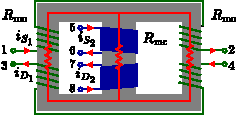
\includegraphics[width=0.6\columnwidth]{Figures_v2/Fig8a.pdf} % Make sure this file exists
        \label{fig:8a}
        }
        \\ % This double backslash forces the next image to the line below (vertical stack)
        % (b) Middle circuit
        \subfloat[]{
        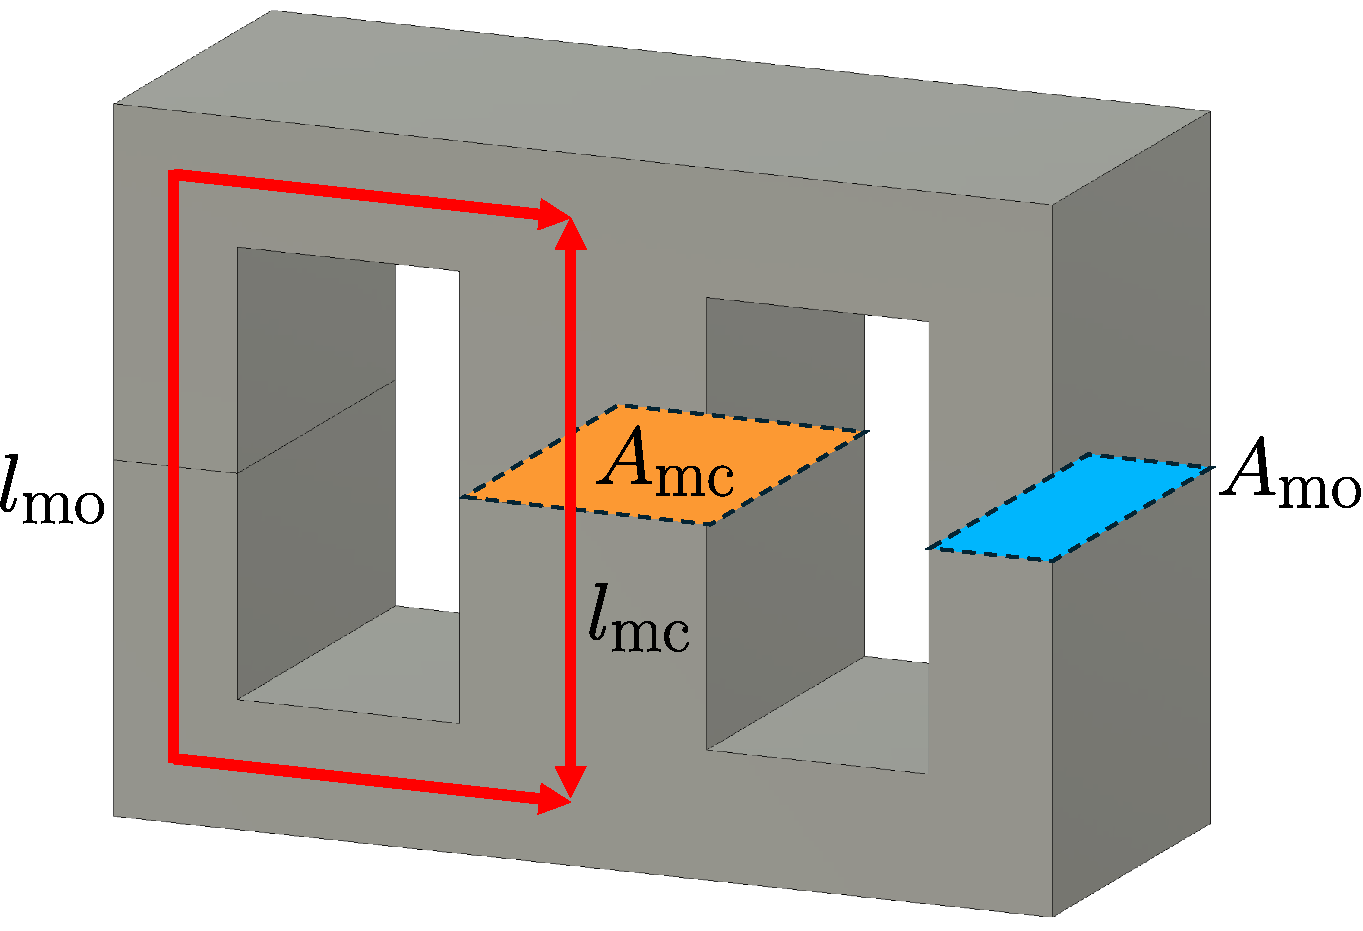
\includegraphics[width=0.75\columnwidth]{Figures_v2/Fig8b.pdf}
        \label{fig:8b}
        }
        
        \caption{EE core configuration: (a) magnetic resistances of the transformer ($R_{\mathrm{mo}}$ for the outer legs, $R_{\mathrm{mc}}$ for the center leg), and (b) effective cross-sectional area ($A_{\mathrm{mo}}$ for the outer legs, $A_{\mathrm{mc}}$ for the center leg) and effective magnetic path length $l_{\mathrm{mo}}$ for the outer legs, $l_{\mathrm{mc}}$ for the center leg.}
\end{figure}

\subsubsection*{\textup{Case 2: $l_{\mathrm{mo}_{\mathrm{air}}} < l_{\mathrm{mc}_{\mathrm{air}}}$}}
Given the setup in Fig. \ref{fig:9b}, $R_{\mathrm{mo}}$ and $R_{\mathrm{mc}}$ are shown in \eqref{eq:23} and \eqref{eq:24} respectively, $l_{\mathrm{mo}_{\mathrm{air}}}$ and $l_{\mathrm{mc}_{\mathrm{air}}}$ in \eqref{eq:25} and \eqref{eq:26} respectively.

\begin{align}
R_{\mathrm{mo}} &= \frac{l_{\mathrm{mo}}}{\mu_r \mu_0 A_{\mathrm{mo}}} + \frac{l_{\mathrm{mo}_{\mathrm{air}}}}{\mu_0 A_{\mathrm{mo}}} \label{eq:23}\\
R_{\mathrm{mc}} &= \frac{l_{\mathrm{mc}} - l_{\mathrm{mc}_{\mathrm{air}}} + l_{\mathrm{mo}_{\mathrm{air}}}}{\mu_r \mu_0 A_{\mathrm{mc}}} + \frac{l_{\mathrm{mc}_{\mathrm{air}}}}{\mu_0 A_{\mathrm{mc}}} \label{eq:24}\\
l_{\mathrm{mo}_{\mathrm{air}}} &= \mu_0 A_{\mathrm{mo}} R_{\mathrm{mo}} - \frac{l_{\mathrm{mo}}}{\mu_r} \label{eq:25}\\
l_{\mathrm{mc}_{\mathrm{air}}} &= \frac{\mu_0 (\mu_r A_{\mathrm{mc}} R_{\mathrm{mc}} - A_{\mathrm{mo}} R_{\mathrm{mo}}) + \frac{l_{\mathrm{mo}}}{\mu_r} - l_{\mathrm{mc}}}{\mu_r - 1} \label{eq:26}
\end{align}

\begin{figure}[b!]
\centering
% (a) Top circuit
        \subfloat[]{
        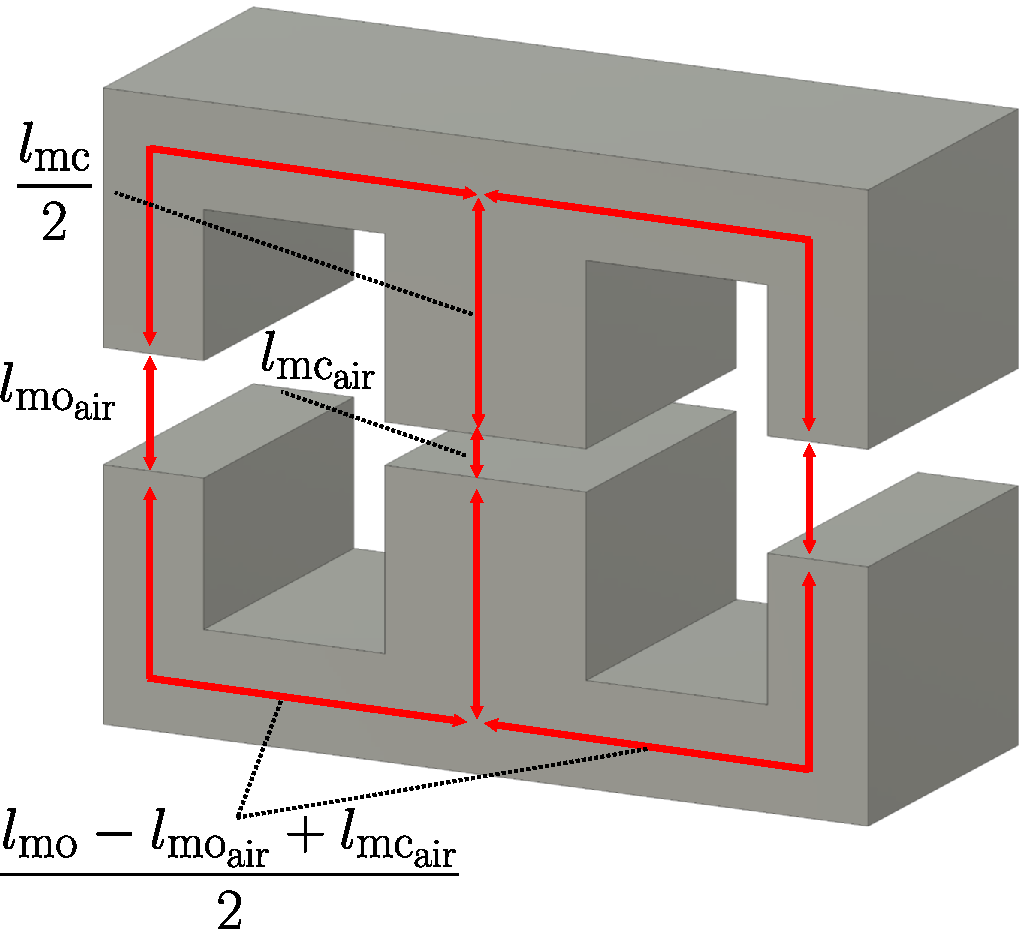
\includegraphics[width=0.7\columnwidth]{Figures_v2/Fig9b.pdf} % Make sure this file exists
        \label{fig:9a}
        }
        \\ % This double backslash forces the next image to the line below (vertical stack)
        % (b) Middle circuit
        \subfloat[]{
        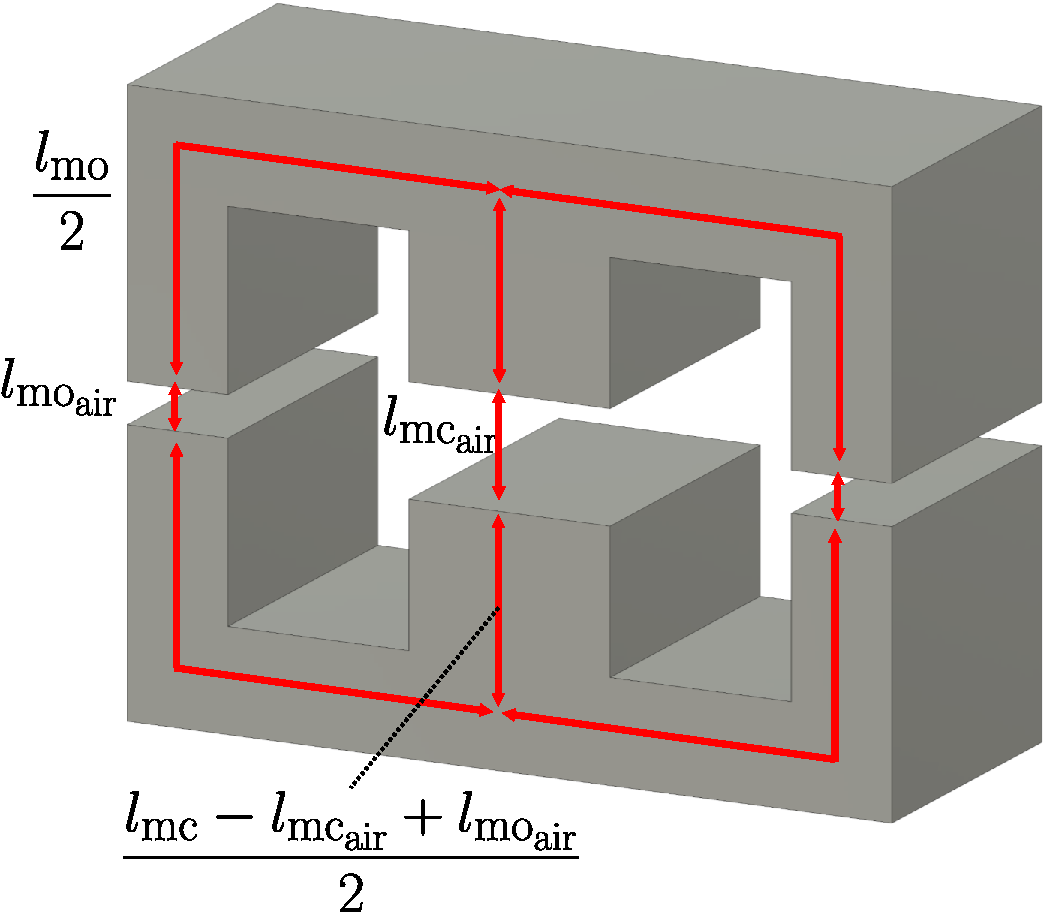
\includegraphics[width=0.7\columnwidth]{Figures_v2/Fig9a.pdf}
        \label{fig:9b}
        }
        
        \caption{EE core configuration with air gaps: (a) setup when $l_{\mathrm{mo}_{\mathrm{air}}} > l_{\mathrm{mc}_{\mathrm{air}}}$ and (b) setup when $l_{\mathrm{mo}_{\mathrm{air}}} < l_{\mathrm{mc}_{\mathrm{air}}}$.}
\end{figure}

\section{Simulation Verification of Proposed Design}
\subsection{Simulation Verification of the Proposed Design Method}
To verify the operation of the integrated transformer, a simulation of the two-phase interleaved flyback rectifier was first performed in PLECS Standalone 4.9.4, with the diagram shown in Fig. \ref{fig:10a}. Clamped RCD Snubbers ($C_{\mathrm{sn}_1}, D_{\mathrm{sn}_1}, R_{\mathrm{sn}_1}$ and $C_{\mathrm{sn}_2}, D_{\mathrm{sn}_2}, R_{\mathrm{sn}_2}$) were also added for protection against surge voltage \cite{ref15, ref16} caused by the leakage inductance and the switch capacitance at the turn-off of $S_1$ and $S_2$. An integrated transformer, shown in Fig. 10(b), was also designed using the proposed method. The circuit and transformer were designed with the condition given by \eqref{eq:8}, and will thus be verified in this study. The specifications of the two-phase interleaved flyback rectifier and transformer for the simulation verification are shown in Tables \ref{tab:sim_rectifier} and \ref{tab:sim_transformer} respectively. 
\begin{figure}[b!]
\centering
% (a) Top circuit
        \subfloat[]{
        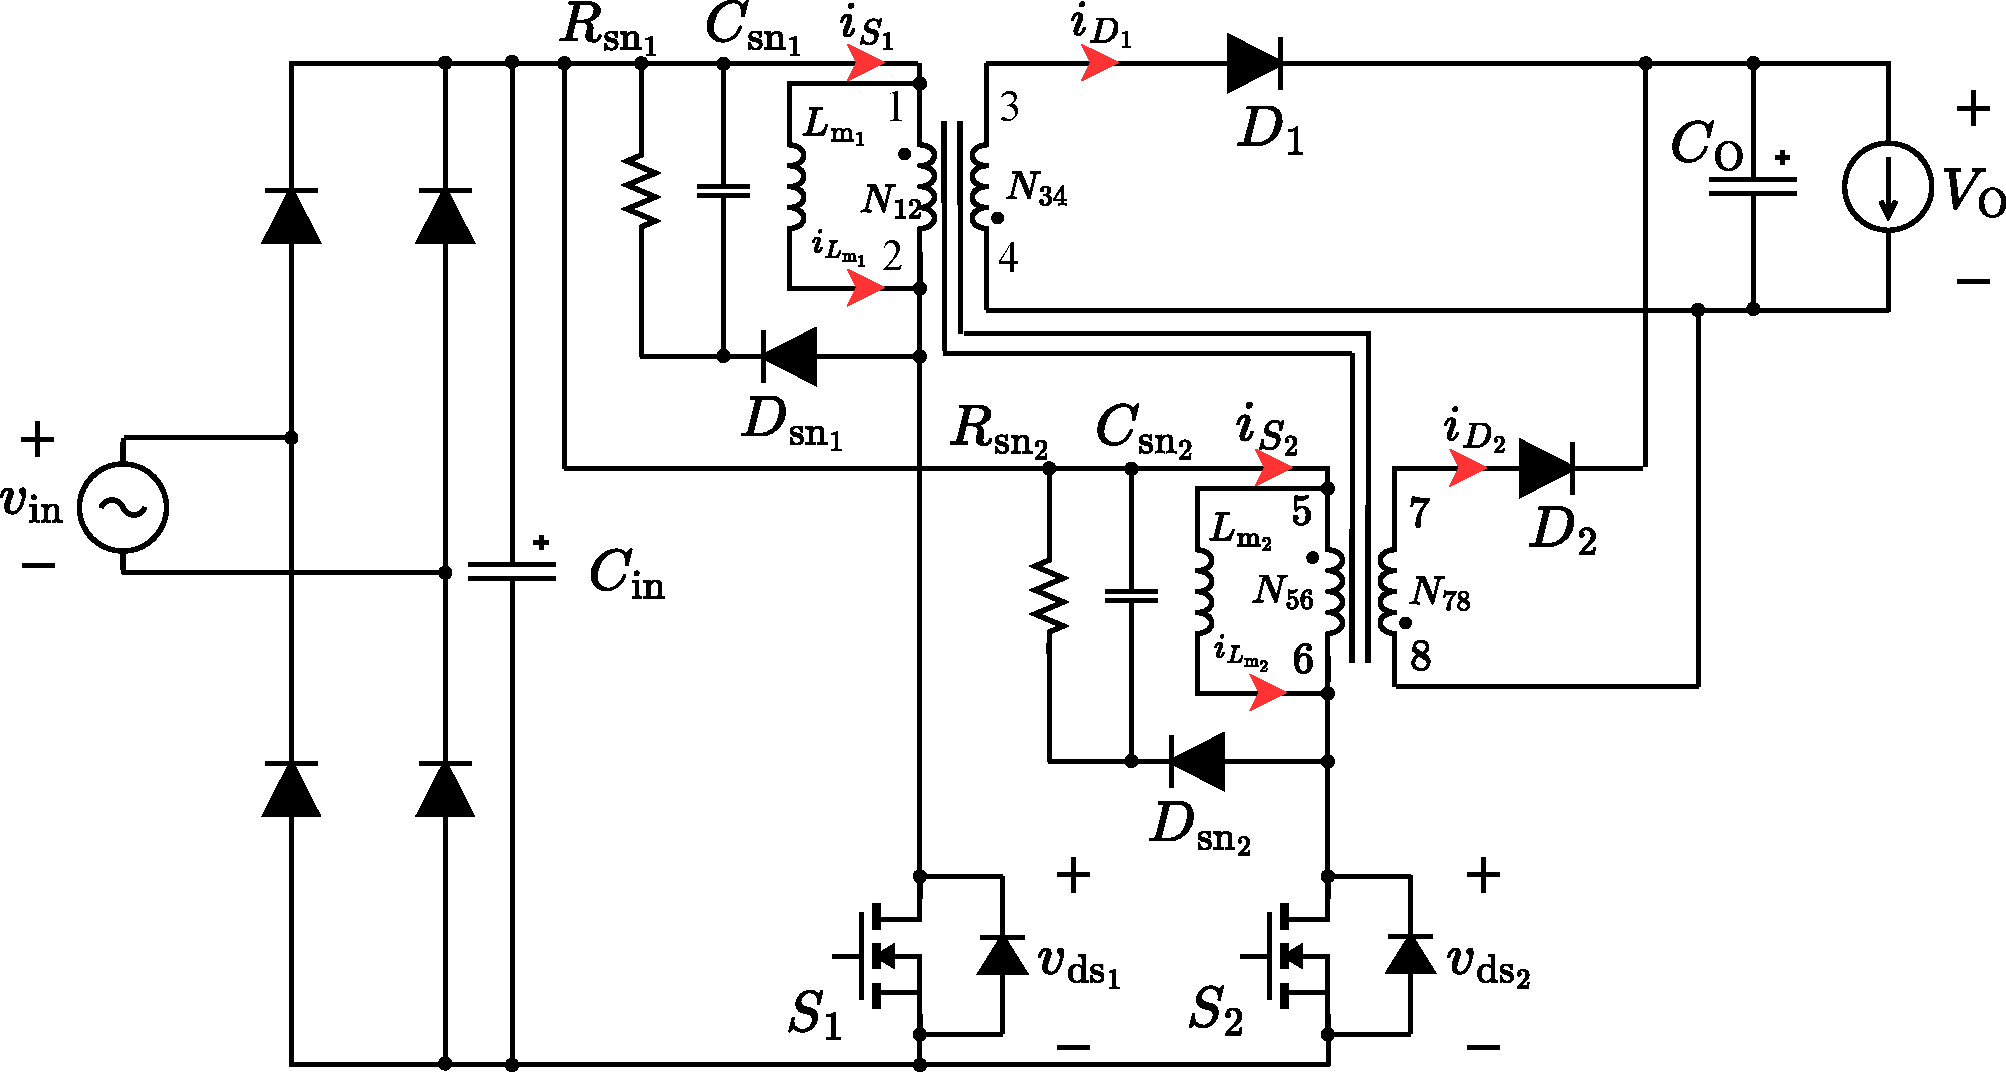
\includegraphics[width=\columnwidth]{Figures_v2/Fig10a.pdf} % Make sure this file exists
        \label{fig:10a}
        }
        \\ % This double backslash forces the next image to the line below (vertical stack)
        % (b) Middle circuit
        \subfloat[]{
        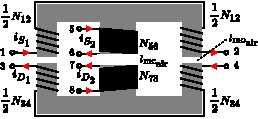
\includegraphics[width=0.6\columnwidth]{Figures_v2/Fig10b.pdf}
        \label{fig:10b}
        }
        
        \caption{Schematic of the: (a) prototype two-phase interleaved flyback rectifier and (b) proposed integrated transformer.}
\end{figure}
\begin{table}[b!]
    \caption{Simulation Specifications of the Prototype Two-Phase Interleaved Flyback Rectifier}
    \centering
    \footnotesize
    \setlength{\tabcolsep}{3pt} % Slightly tighter spacing to handle long text
    \begin{tabular}{ccc}
        \hline
        \textbf{Item} & \textbf{Symbol} & \textbf{Value} \\
        \hline \hline
        AC input voltage & $v_{\mathrm{in}}$ & 100 V$_{\textrm{rms}}$\\
        Maximum rated power & $P_{\mathrm{O}}$ & 240 W \\
        Output voltage & $V_{\mathrm{O}}$ & 48 V \\
        Switching frequency & $f_{\mathrm{s}}$ & 100 kHz \\
        Input capacitor & $C_{\mathrm{in}}$ & 1 \textmu F \\
        Output capacitor & $C_{\mathrm{O}}$ & 2 x 1mF (parallel) \\
        Snubber capacitor & $C_{\mathrm{sn}_1}, C_{\mathrm{sn}_2}$ & 2.2 nF \\
        Snubber resistor & $R_{\mathrm{sn}_1}, R_{\mathrm{sn}_2}$ & 30 k$\Omega$ \\
        \hline
    \end{tabular}
    \label{tab:sim_rectifier}
\end{table}

\begin{table}[t!]
    \caption{Simulation Specifications of the Prototype Integrated Transformer}
    \centering
    \footnotesize
    \setlength{\tabcolsep}{4pt} 
    \begin{tabular}{ccc}
        \hline
        \textbf{Item} & \textbf{Symbol} & \textbf{Value} \\
        \hline \hline
        Magnetic core & - & OP44721EC \\
        Relative permeability & $\mu_r$ & 2500\\
        Magnetic path length (center leg) & $l_{\mathrm{mc}}$ & 31.7 mm\\
        Magnetic path length (outer leg) & $l_{\mathrm{mo}}$ & 71.4 mm\\
        Cross-sectional area (center leg) & $A_{\mathrm{mc}}$ & 243.4 mm$^2$ \\
        Cross-sectional area (outer leg) & $A_{\mathrm{mo}}$ & 117.6 mm$^2$\\
        Magnetizing inductance & $L_{\mathrm{m}_1}, L_{\mathrm{m}_2}$ & 82.8 \textmu H \\
        Turn ratio & $n$ & 3 \\
        \multirow{2}{*}{Number of turns} & $N_{12}:N_{34}$ & 24:8 \\
                                         & $N_{56}:N_{78}$ & 18:6 \\
        Center leg air gap & $l_{{\mathrm{mc}}_{\mathrm{air}}}$ & 0.650 mm \\
        Outer leg air gap & $l_{{\mathrm{mo}}_{\mathrm{air}}}$ & 0.500 mm \\
        Coupling coefficient of $N_{12}, N_{34}$ & $k_{N_{12}-N_{34}}$ & 0.990 \\
        Coupling coefficient of $N_{56}, N_{78}$ & $k_{N_{56}-N_{78}}$ & 0.990 \\
        Coupling coefficient of $N_{12}, N_{56}$ & $k_{N_{12}-N_{56}}$ & 0.000 \\
        \hline
    \end{tabular}
    \label{tab:sim_transformer}
\end{table}



\subsection{Simulation Results}
Fig. \ref{fig:11} shows waveforms from the simulation testing of the two-phase interleaved flyback rectifier with the proposed transformer at 240 W. Key waveforms of the circuit were observed from the simulation, which include $v_{\mathrm{gs}_1}$ and $v_{\mathrm{gs}_2}$, $i_{L_{\mathrm{m}_1}}$ and $i_{L_{\mathrm{m}_2}}$, and the fluxes $B_{\mathrm{o}_1}$, $B_{\mathrm{o}_2}$, and $B_{\mathrm{c}}$. Similar waveforms to that of Fig. \ref{fig:4} have been observed, confirming that the system operates exactly as expected from the theoretical analysis. Flux cancellation is observed in the center leg during the time that $N_{56}-N_{78}$ is inactive, as denoted by the interval when $i_{L_{\mathrm{m}_2}} = 0$. The magnetizing currents $i_{L_{\mathrm{m}_1}}$ and $i_{L_{\mathrm{m}_2}}$ subside to zero prior to the subsequent phase reaching its peak. Moreover, the increase and decrease of fluxes were all linear, therefore confirming that there is indeed no magnetic coupling interference. This confirms the validity of the theoretical operation proposed in Section II.

\begin{figure}[t!]
    % Import the separate file here
    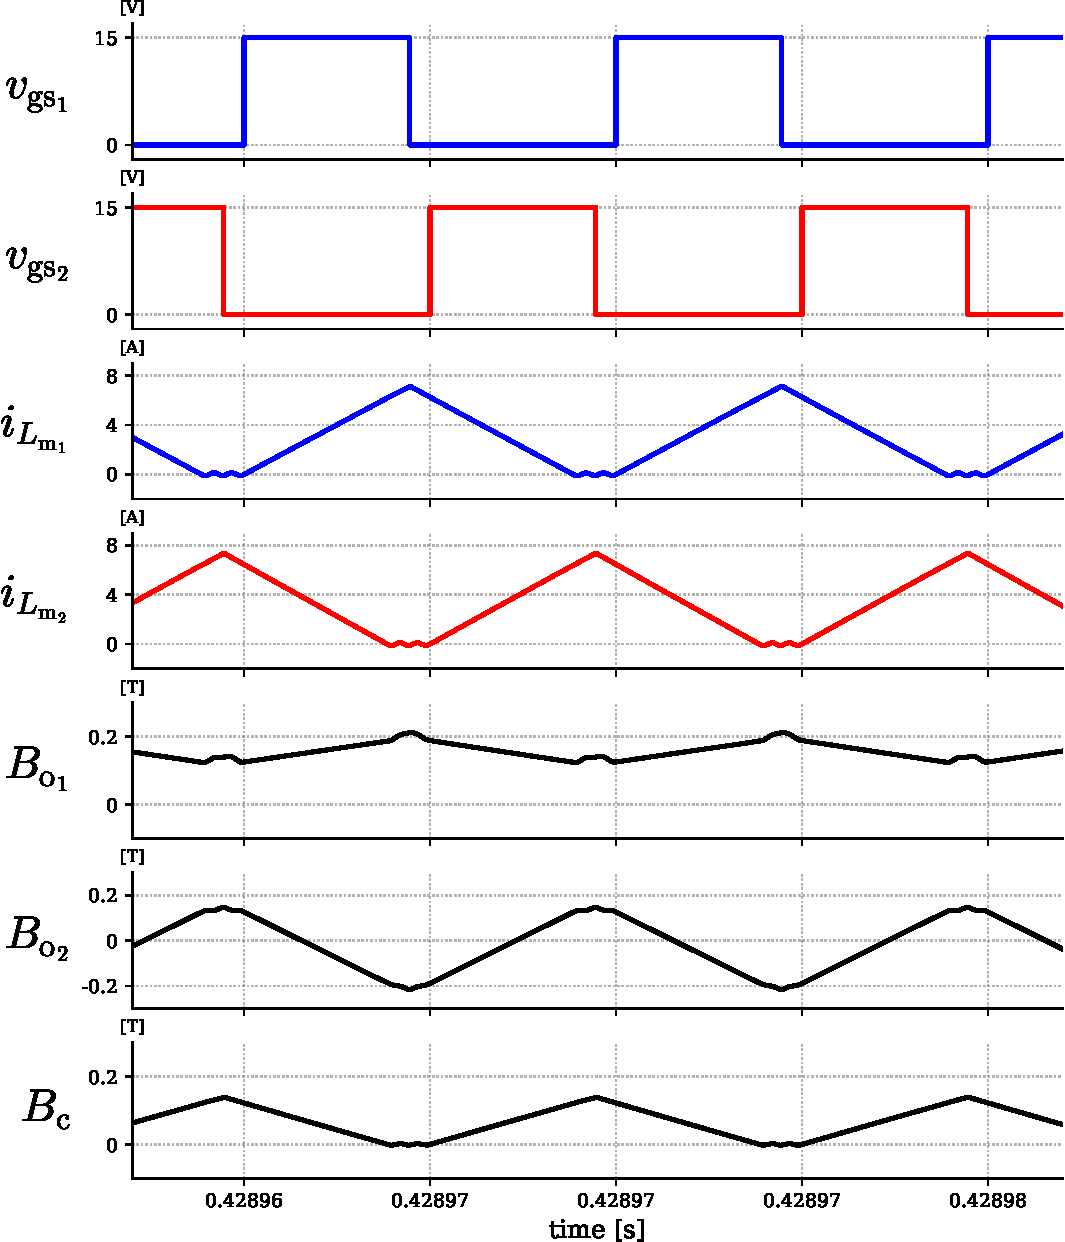
\includegraphics[width=\columnwidth]{Figures_v2/sim_plot_output.pdf}
    \caption{Key simulation waveforms of the proposed two-phase interleaved flyback rectifier at 240 W.}
    \label{fig:11}
\end{figure}

Furthermore, to substantiate the power factor correction capability of the proposed integrated structure, an open-loop performance analysis was conducted across the universal input range. To establish a rigorous baseline for this evaluation, a conventional two-phase interleaved flyback rectifier utilizing two separate, discrete transformers was also simulated. To ensure a strictly fair comparison, the physical parameters of the discrete transformers were precisely matched to the proposed design. The cross-sectional area of the discrete cores was matched to the smaller outer leg of the proposed core, $A_\mathrm{mo} = 117.624 \text{ mm}^2$. The discrete transformers were assigned identical turns ratios to the center leg transformer of the proposed integrated component 18:6, and their air gaps were tuned to maintain the exact same nominal magnetizing inductance $L_\mathrm{m}$. For the discrete cores, the magnetic path length was set to $66.21 \text{ mm}$ with an air gap of $0.677 \text{ mm}$. To extract clean grid-side AC waveforms and accurately evaluate harmonic distortion, a standard differential-mode EMI filter ($L_f = 100 \text{~\textmu H}$, $C_f = 1 \text{~\textmu F}$) was incorporated into both simulation models.

As summarized in Table \ref{tab:pf_thd_comparison}, the proposed non-coupled integrated transformer maintains a high power factor of $>0.95$ and low current THD across various input voltages and load conditions. Crucially, the fundamental decoupling of the magnetic structure ensures that its PF and THD performance remains nearly identical to that of the conventional discrete implementation and aditionally validates the claims of inherent PFC operation in DCM in Section II. To provide a clear visual reference of this capability, the simulated PFC waveforms at the operating points of $v_\mathrm{in}$, $V_\mathrm{O}$, and $P_\mathrm{O}$ of 100 V$_\mathrm{rms}$, 48 V, and 100 W, and 240 V$_\mathrm{rms}$, 48 V, and 100 W  are shown in Fig. \ref{fig:pfca} and \ref{fig:pfcb}.

\begin{table}[htbp]
    \caption{Power Factor and THD Comparison (Open-Loop Simulation)}
    \centering
    \renewcommand{\arraystretch}{1.25} % Adds vertical breathing room to all rows
    \begin{tabular}{c c c c c}
        \hline
        \multirow{2}{*}{\begin{tabular}[c]{@{}c@{}}\textbf{Operating Point} \\ ($V_{\text{in}}$, $V_{\text{out}}$, $P_{\text{O}}$)\end{tabular}} & \multicolumn{2}{c}{\textbf{Power Factor}} & \multicolumn{2}{c}{\textbf{Current THD (\%)}} \\
        \cline{2-5}
        & \textbf{Conv.} & \textbf{Prop.} & \textbf{Conv.} & \textbf{Prop.} \\
        \hline \hline
        100 V$_{\text{rms}}$, 48 V, 240 W & 0.9991 & 0.9987 & 2.39 & 2.19 \\
        240 V$_{\text{rms}}$, 48 V, 240 W & 0.9758 & 0.9641 & 4.34 & 4.02 \\
        100 V$_{\text{rms}}$, 20 V, 100 W & 0.9918 & 0.9932 & 3.42 & 2.43 \\
        100 V$_{\text{rms}}$, 12 V, 45 W  & 0.9724 & 0.9567 & 3.59 & 3.51 \\
        \hline
    \end{tabular}
    \label{tab:pf_thd_comparison}
\end{table}

\begin{figure}[htbp]
\centering
% (a) Top circuit
        \subfloat[]{
        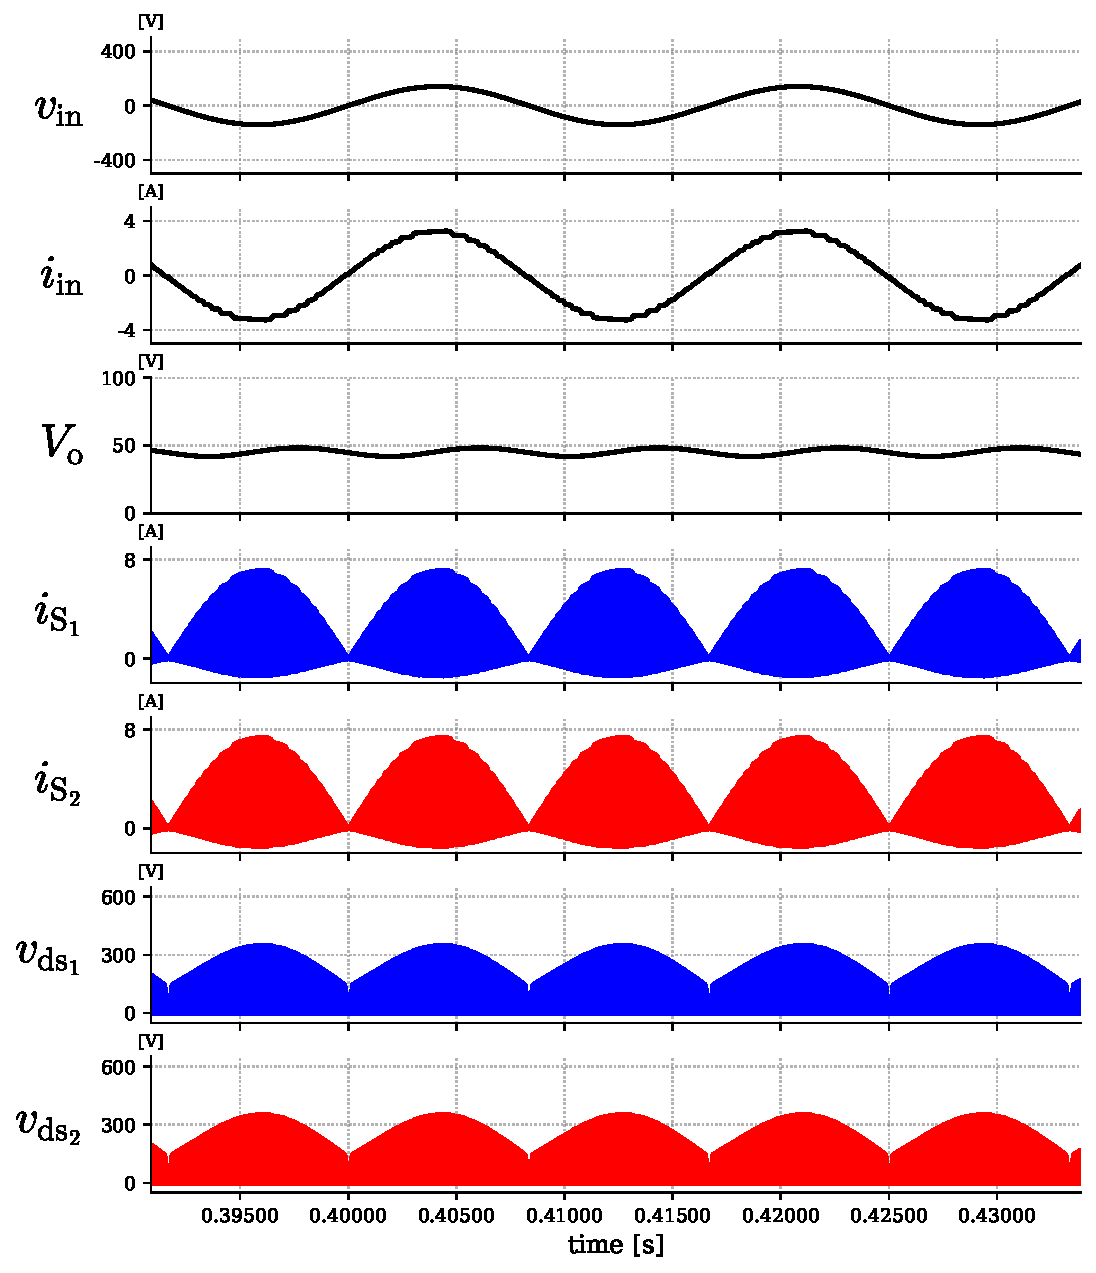
\includegraphics[width=\columnwidth]{Figures_v2/sim_plot_output_100.pdf} % Make sure this file exists
        \label{fig:pfca}
        }
        \\ % This double backslash forces the next image to the line below (vertical stack)
        % (b) Middle circuit
        \subfloat[]{
        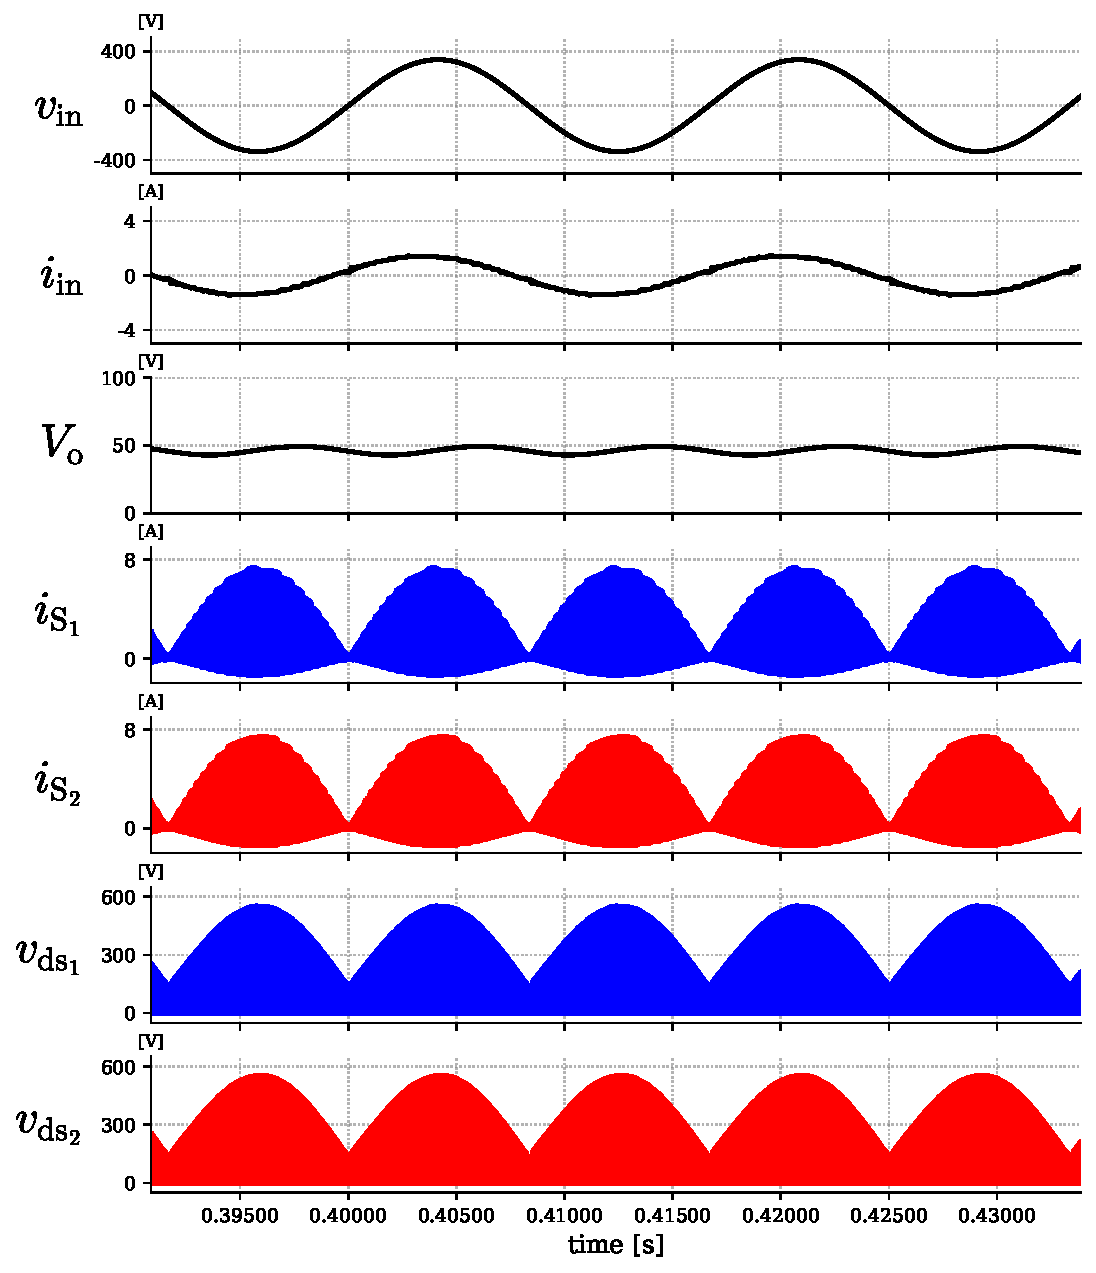
\includegraphics[width=\columnwidth]{Figures_v2/sim_plot_output_240.pdf}
        \label{fig:pfcb}
        }
        
        \caption{Key PFC Waveforms with $v_\mathrm{in}$, $V_\mathrm{O}$, and $P_\mathrm{O}$ of: (a) 100 V$_\mathrm{rms}$, 48 V, and 240 W and (b) 240 V$_\mathrm{rms}$, 48 V, and 240 W.}
        \label{fig:pfcwaveforms}
\end{figure}


\section{Size Reduction Effect of the Proposed Transformer}
This section examines the size reduction effect by the integrated transformer. For this study, the conventional transformer is assumed to be two separate transformers that facilitate isolation between the primary and secondary side. The conventional transformer and its windings is represented in Fig.~\ref{fig:13a}. The proposed integrated transformer and its windings is represented in Fig.~\ref{fig:13b}. The volume is compared by using the AP method. The AP method utilizes the product between the core cross-sectional area $A_{\mathrm{c}}$, and the window area $A_{\mathrm{w}}$, and is a fundamental core size for the application \cite{ref21}. It can be expressed both in terms of the transformer geometric parameters and the circuit parameters, as will be demonstrated in the following analysis.

\begin{figure}[t!]
\centering
% (a) Top circuit
        \subfloat[]{
        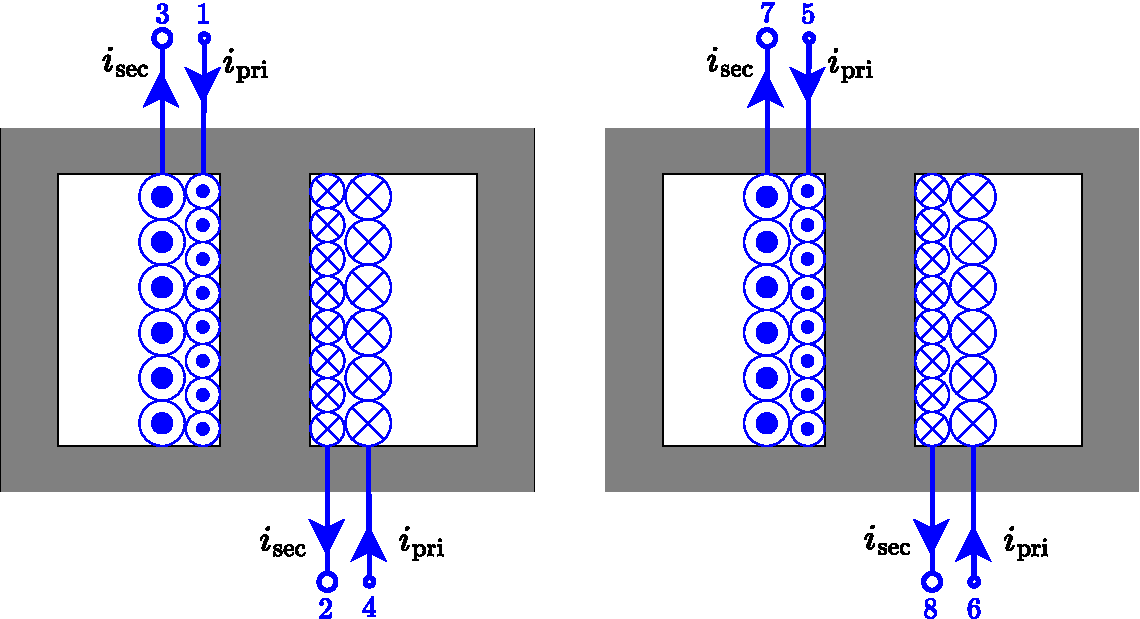
\includegraphics[width=0.9\columnwidth]{Figures_v2/Fig13a.pdf} % Make sure this file exists
        \label{fig:13a}
        }
        \\ % This double backslash forces the next image to the line below (vertical stack)
        % (b) Middle circuit
        \subfloat[]{
        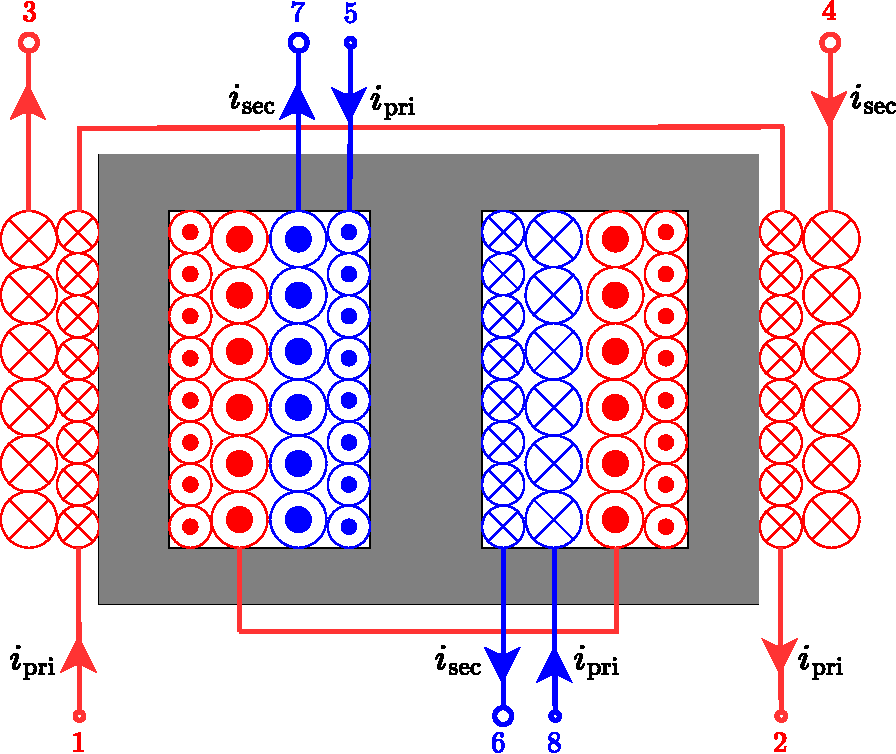
\includegraphics[width=0.7\columnwidth]{Figures_v2/Fig13b.pdf}
        \label{fig:13b}
        }
        
        \caption{Two separate transformers (a) and the proposed integrated transformer (b) used in the volume analysis, with the windings represented as well.}
        \label{fig:13}
\end{figure}


The EE-core was redesigned such that $A_{\mathrm{w}}$ and $A_{\mathrm{c}}$ are squares to allow for simpler analysis, as shown in Fig.~\ref{fig:14} \cite{ref22}. Here, $A_{\mathrm{c}}$ is twice the area of the outer leg.

\begin{figure}[b!]
\centering
        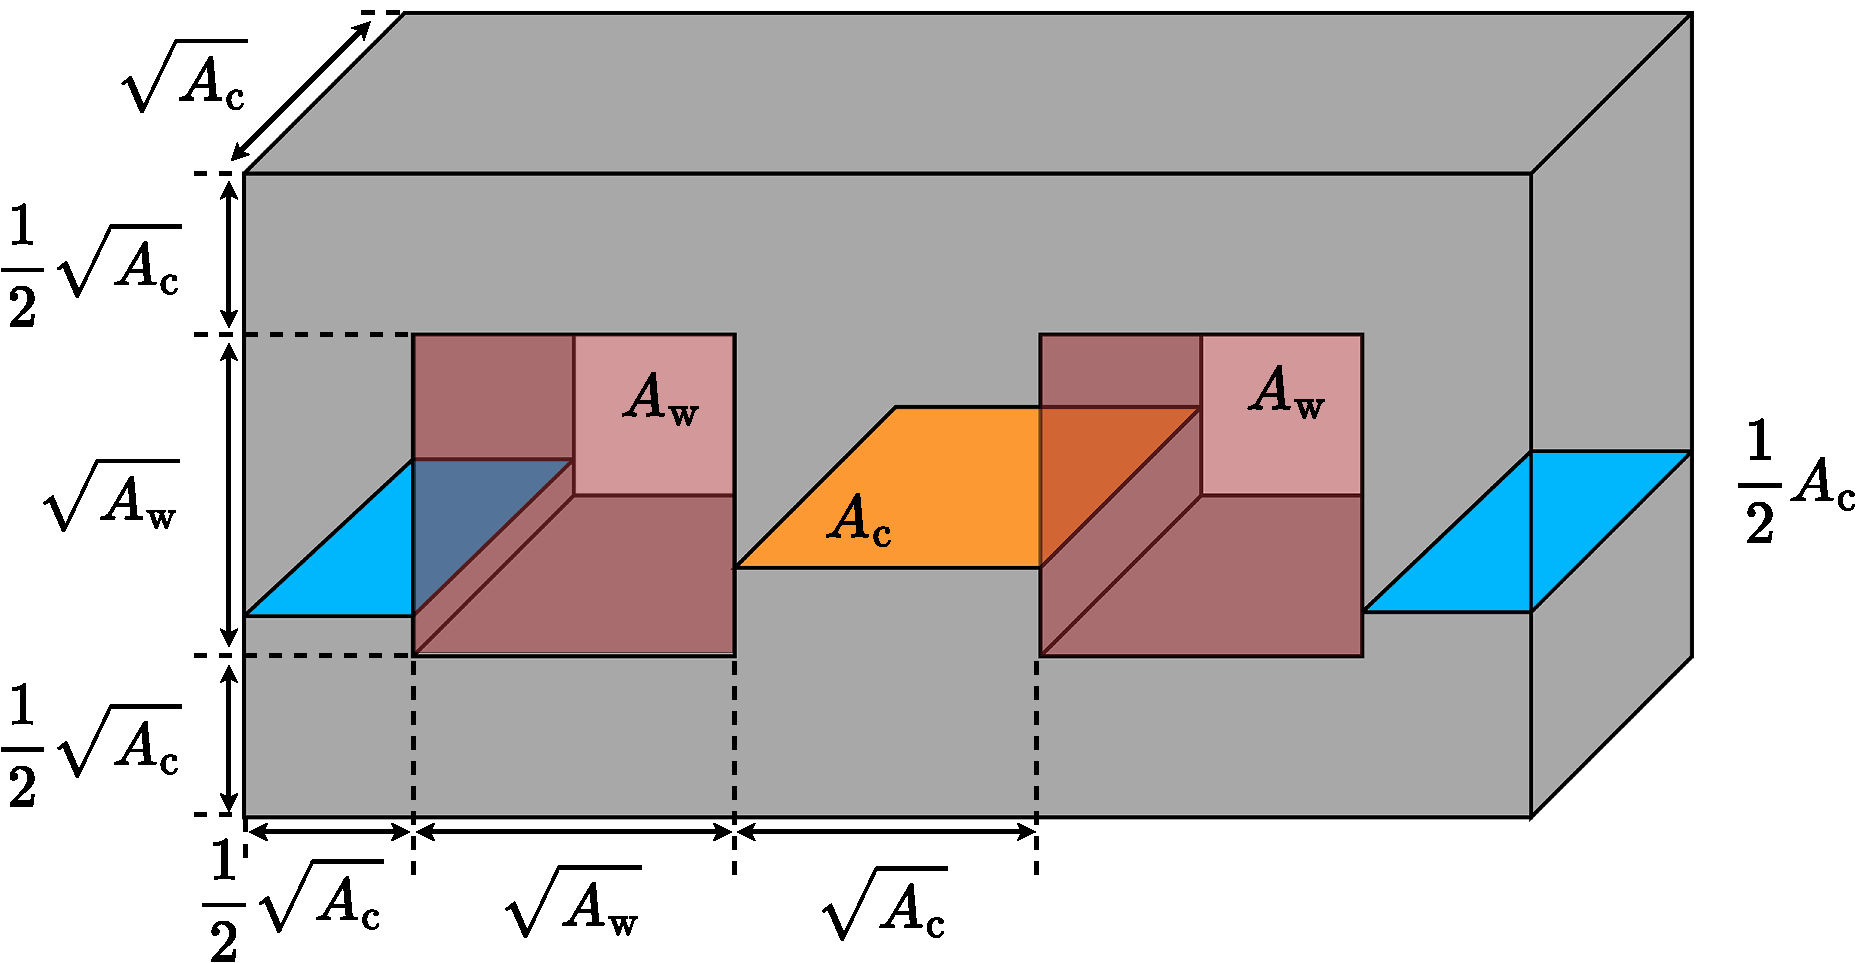
\includegraphics[width=\columnwidth]{Figures_v2/Fig14.pdf} % Make sure this file exists
        
        \caption{Simplified representation of one EE-core used in the volume analysis.}
        \label{fig:14}
\end{figure}

For the conventional transformer, $A_{\mathrm{c}}$ is expressed in \eqref{eq:Ac_conv}. Here, $N_{\mathrm{p}}$ is the number of turns wound on the center leg of the conventional transformer.
\begin{equation}
\label{eq:Ac_conv}
A_{\mathrm{c}_{\mathrm{conv}}} = \frac{L_{\mathrm{m}} I_{\mathrm{pri}_{\mathrm{pk}}}}{B_{\mathrm{max}} N_{\mathrm{p}}}
\end{equation}

For the integrated transformer, $A_{\mathrm{c}}$ is expressed in \eqref{eq:Ac_integ}.
\begin{equation}
\label{eq:Ac_integ}
A_{\mathrm{c}_{\mathrm{integ}}} = \frac{L_{\mathrm{m}} I_{\mathrm{pri}_{\mathrm{pk}}}}{B_{\mathrm{max}} N_{56}}
\end{equation}

The window area $A_{\mathrm{w}}$ can be expressed in terms of winding area and the occupancy ratio $K_{\mathrm{u}}$, as seen in \eqref{eq:Aw_conv1} for the conventional transformer:
\begin{equation}
\label{eq:Aw_conv1}
A_{\mathrm{w}_{\mathrm{conv}}} K_{\mathrm{u}} = N_{\mathrm{p}} \frac{I_{\mathrm{pri}_{\mathrm{rms}}}}{J_{\mathrm{m}}} + N_{\mathrm{s}} \frac{I_{\mathrm{sec}_{\mathrm{rms}}}}{J_{\mathrm{m}}}
\end{equation}
which simplifies to:
\begin{equation}
\label{eq:Aw_conv2}
A_{\mathrm{w}_{\mathrm{conv}}} = \frac{N_{\mathrm{p}}}{J_{\mathrm{m}} K_{\mathrm{u}}} \left(I_{\mathrm{pri}_{\mathrm{rms}}} + \frac{I_{\mathrm{sec}_{\mathrm{rms}}}}{n}\right)
\end{equation}

For the integrated transformer, winding $N_{12}$ and $N_{34}$ on the outer legs implies that $N_{12} \approx 2N_{56}$ and $N_{34} \approx 2N_{78}$. Taking into account that the core window has half the total turns of the transformer $N_{12}-N_{34}$, $A_{\mathrm{w}}$ can be expressed as \eqref{eq:Aw_integ}:
\begin{align}
\label{eq:Aw_integ}
A_{\mathrm{w}_{\mathrm{integ}}} K_{\mathrm{u}} &= \left(N_{56} \frac{I_{\mathrm{pri}_{\mathrm{rms}}}}{J_{\mathrm{m}}} + N_{78} \frac{I_{\mathrm{sec}_{\mathrm{rms}}}}{J_{\mathrm{m}}}\right) \nonumber \\
&\quad + \frac{1}{2}\left(N_{12} \frac{I_{\mathrm{pri}_{\mathrm{rms}}}}{J_{\mathrm{m}}} + N_{34} \frac{I_{\mathrm{sec}_{\mathrm{rms}}}}{J_{\mathrm{m}}}\right) \nonumber \\
&= 2 \left( \frac{N_{56} I_{\mathrm{pri}_{\mathrm{rms}}}}{J_{\mathrm{m}}} + \frac{N_{78} I_{\mathrm{sec}_{\mathrm{rms}}}}{J_{\mathrm{m}}} \right) 
\end{align}

Using \eqref{eq:Ac_conv}, \eqref{eq:Ac_integ}, \eqref{eq:Aw_conv2}, and \eqref{eq:Aw_integ}, the AP of the conventional and proposed integrated transformers are expressed in \eqref{eq:AP_conv} and \eqref{eq:AP_integ} respectively:
\begin{align}
\label{eq:AP_conv}
AP_{\mathrm{conv}} &= A_{\mathrm{c}_{\mathrm{conv}}} A_{\mathrm{w}_{\mathrm{conv}}} \nonumber \\ &=\frac{L_{\mathrm{m}} I_{\mathrm{pri}_{\mathrm{pk}}} \left( I_{\mathrm{pri}_{\mathrm{rms}}} + \frac{I_{\mathrm{sec}_{\mathrm{rms}}}}{n} \right)}{B_{\mathrm{max}} J_{\mathrm{m}} K_{\mathrm{u}}}
\end{align}

\begin{align}
\label{eq:AP_integ}
AP_{\mathrm{integ}} &= A_{\mathrm{c}_{\mathrm{integ}}} A_{\mathrm{w}_{\mathrm{integ}}} \nonumber \\ &= \frac{2 L_{\mathrm{m}} I_{\mathrm{pri}_{\mathrm{pk}}} \left( I_{\mathrm{pri}_{\mathrm{rms}}} + \frac{I_{\mathrm{sec}_{\mathrm{rms}}}}{n} \right)}{B_{\mathrm{max}} J_{\mathrm{m}} K_{\mathrm{u}}}
\end{align}

From \eqref{eq:AP_conv} and \eqref{eq:AP_integ}, $AP_{\mathrm{integ}} \approx 2 AP_{\mathrm{conv}}$ ideally.

The total volume of the EE core in Fig.~\ref{fig:14} is expressed in \eqref{eq:Vol}, where $x$ is a constant that denotes $A_{\mathrm{c}}/A_{\mathrm{w}}$. The volume corresponding to the conventional and integrated transformer is obtained using their respective $A_{\mathrm{c}}$ and $A_{\mathrm{w}}$. Since the $A_{\mathrm{c}}$ and $A_{\mathrm{w}}$ depend on the number of corresponding turns, then the estimated volume will change depending on the actual implementation of the transformer.
\begin{equation}
\label{eq:Vol}
\mathrm{Vol} = 2 AP^{\frac{3}{4}} \left(2 x^{\frac{1}{4}} + x^{\frac{3}{4}} + x^{-\frac{1}{4}}\right)
\end{equation}

Also, the $A_{\mathrm{c}}$ and $A_{\mathrm{w}}$ can be expressed in terms of the AP and $x$ as shown in \eqref{eq:Ac_new} and \eqref{eq:Aw_new}:
\begin{equation}
\label{eq:Ac_new}
A_{\mathrm{c}} = \sqrt{x \cdot AP}
\end{equation}

\begin{equation}
\label{eq:Aw_new}
A_{\mathrm{w}} = \sqrt{\frac{AP}{x}}
\end{equation}

The rms expressions of the primary and secondary side current of the interleaved flyback rectifier are given in \eqref{eq:Irms_pri} and \eqref{eq:Irms_sec} \cite{ref8}.
\begin{align}
I_{\mathrm{pri}_{\mathrm{rms}}} &= \frac{V_{\mathrm{in}_{\mathrm{max}}}}{L_{\mathrm{m}} f_{\mathrm{s}}} \sqrt{\frac{D^3}{6}} \label{eq:Irms_pri}\\
I_{\mathrm{sec}_{\mathrm{rms}}} &= \frac{V_{\mathrm{in}_{\mathrm{max}}}}{L_{\mathrm{m}} f_{\mathrm{s}}} \sqrt{\frac{4 n D^3}{9 \pi} \cdot \frac{V_{\mathrm{in}_{\mathrm{max}}}}{V_{\mathrm{o}}}} \label{eq:Irms_sec}
\end{align}

The AP calculation based on circuit specifications is summarized in Table~\ref{tab:volume}. The conventional transformer implementation comprises of two discrete cores, the value indicated in this table is for one core only.

\begin{table}[b!]
    \caption{Area Products of the Conventional (1 core) and Proposed Integrated Transformer}
    \centering
    \footnotesize
    \setlength{\tabcolsep}{2pt}
    \begin{tabular}{cccc}
        \hline
        \textbf{Item} & \textbf{Symbol} & \textbf{Conventional (1 core)} & \textbf{Proposed} \\
        \hline \hline
        Maximum input voltage & $V_{\mathrm{in}_{\mathrm{max}}}$ & \multicolumn{2}{c}{240 V$_{\mathrm{rms}}$} \\
        Output voltage & $V_{\mathrm{O}}$ & \multicolumn{2}{c}{48 V} \\
        Maximum duty cycle & $D$ & \multicolumn{2}{c}{0.47} \\
        Switching frequency & $f_\mathrm{s}$ & \multicolumn{2}{c}{100 kHz} \\
        \hline
        Magnetizing inductance & $L_{\mathrm{m}}$ & \multicolumn{2}{c}{82.8 \textmu H} \\
        Turn ratio & $n$ & \multicolumn{2}{c}{3} \\
        % --- SHARED PARAMETERS ---
        Primary side peak current & $I_{\mathrm{pri,pk}}$ & \multicolumn{2}{c}{8.02 A} \\
        Primary side rms current & $I_{\mathrm{pri,rms}}$ & \multicolumn{2}{c}{5.39 A} \\
        Secondary side rms current & $I_{\mathrm{sec,rms}}$ & \multicolumn{2}{c}{12.53 A} \\
        Saturation flux density & $B_{\mathrm{max}}$ & \multicolumn{2}{c}{0.3 T} \\
        Maximum current density & $J_{\mathrm{m}}$ & \multicolumn{2}{c}{5 A/mm$^2$} \\
        Occupancy ratio & $K_{\mathrm{u}}$ & \multicolumn{2}{c}{0.3} \\
        \hline
        Area Product & $\mathrm{AP}$ & 14128.75 mm$^4$ & 28257.50 mm$^4$ \\
        \hline
    \end{tabular}
    \label{tab:volume}
\end{table}

The theoretical volume is dominated by the $AP^{3/4}$ scaling law as seen in \eqref{eq:Vol}, and thus the term $\left( 2x^{1/4} + x^{3/4} + x^{-1/4} \right)$ can be treated as constant. Using the relationship $AP_{\mathrm{integ}} \approx 2 AP_{\mathrm{conv}}$, then the amount of volume reduction can be computed using \eqref{eq:Vol}, with the reduction amounting to 16\%. This assumes that the integrated core geometry is custom-tailored to the specific AP requirements derived from the circuit specifications, rather than being constrained by standard commercial core shapes. While the experimental prototype described in Section V utilizes a commercial core (Magnetics 0P44721EC) for proof-of-concept, this theoretical analysis confirms that a purpose-built integrated core would offer significant improvements in power density compared to the conventional discrete implementation by standard commercial core shapes.

While the proposed integrated transformer achieves a theoretical 16\% reduction in core volume, this structural integration introduces some trade-offs regarding core and winding losses.

In a conventional discrete setup, the flux density remains uniform across the isolated magnetic paths. In contrast, the proposed integrated core shares flux paths, resulting in a complex flux distribution due to the superposition of individual phase contributions. As established in the theoretical waveforms of Fig.~\ref{fig:flux_waveforms}, overlapping conduction intervals create localized regions of high flux density (additive flux) in one outer leg, while simultaneously creating regions of reduced flux density (subtractive flux) in the opposite outer leg. Because core loss scales non-linearly with flux density, the net impact on the total core loss involves both mitigating and compounding factors, necessitating rigorous analysis for full volumetric loss integration in future optimization stages.

Furthermore, the geometry of the shared EE-core forces a structural asymmetry in the windings. To balance the magnetizing inductance, the outer legs require an increased turn count compared to a conventional discrete transformer. Although the smaller physical perimeter of the outer legs partially offsets the DC resistance penalty of these additional turns, the high-frequency AC resistance $R_{\mathrm{ac}}$ remains highly dependent on the physical layering and winding arrangement. Consequently, achieving optimal winding efficiency requires careful geometric optimization and parameter sweeping, which is a critical focus for the future phases of this study.

\section{Experimental Verification of Proposed Design}

\subsection{Prototype Flyback Circuit and Integrated Transformer}

A prototype two-phase interleaved flyback rectifier, with the circuit schematic shown in Fig.~\ref{fig:10a}, was built to verify the operation of the integrated transformer operating in DCM. A photograph of the prototype evaluation board is provided in Fig.~\ref{fig:pcb}, with the primary and secondary side separated for simple implementation. Because the fundamental operating principles of the converter remain identical to a conventional discrete setup, standard closed-loop modulation methods are directly applicable. Therefore, the experimental evaluation was intentionally conducted using open-loop control with a fixed duty cycle decided using \eqref{eq:27}.

\begin{figure}[b!]
\centering
        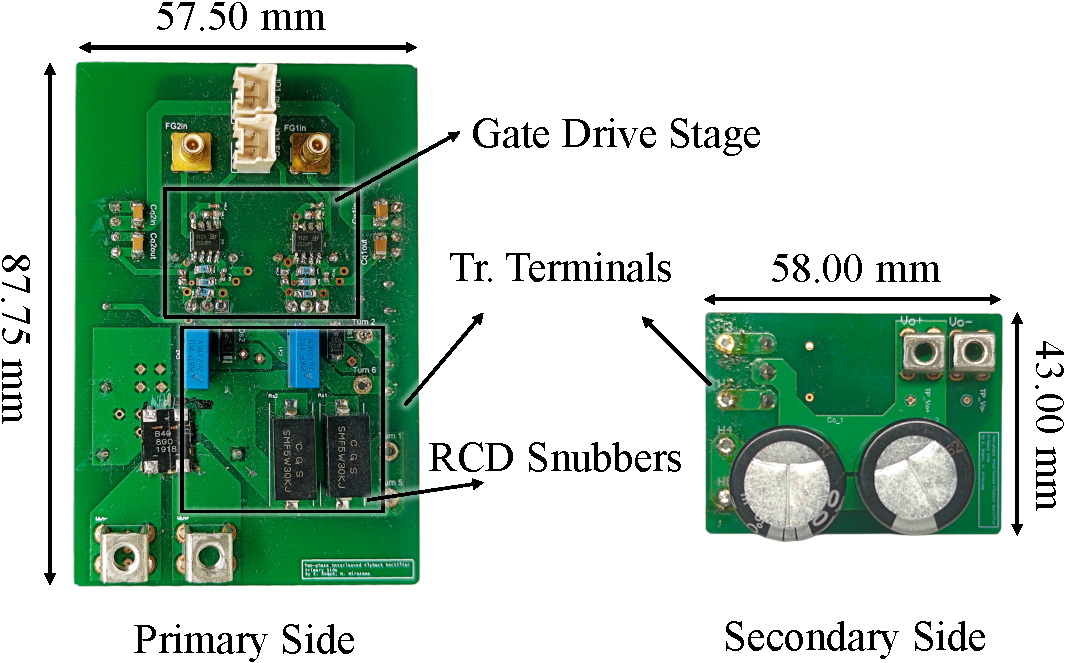
\includegraphics[width=0.82\columnwidth]{Figures_v2/pcb.pdf} % Make sure this file exists
        \caption{Photograph of the evaluation board for the proposed integreated flyback PFC rectifier.}
        \label{fig:pcb}
\end{figure}

The prototype integrated transformer, represented in Fig.~\ref{fig:10b}, was also designed using the proposed method. To strictly minimize leakage inductance, the primary and secondary windings of the transformer for each respective phase were physically overlapped on their designated legs. The EE-core used for the prototype is shown in Fig.~\ref{fig:core}. The windings are wound around lab-made coil formers, as shown in Fig.~\ref{fig:bobbin}, which were fabricated using a Flashforge Adventurer 4 Series 3D printer, and are finally placed onto the corresponding legs of the core. A photograph of the fully assembled prototype integrated transformer is shown in Fig.~\ref{fig:trans}. The specifications of the two-phase interleaved flyback rectifier and transformer are shown in Tables~\ref{tab:prototype_rectifier} and \ref{tab:prototype_transformer}, respectively. 

\begin{figure}[t!]
\centering
% (a) Top circuit
        \subfloat[]{
        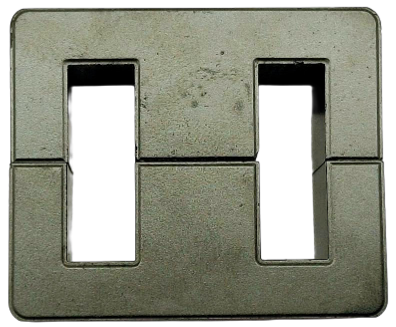
\includegraphics[width=0.4\columnwidth]{Figures_v2/core.pdf} % Make sure this file exists
        \label{fig:core}
        }
        \\ % This double backslash forces the next image to the line below (vertical stack)
        % (b) Middle circuit
        \subfloat[]{
        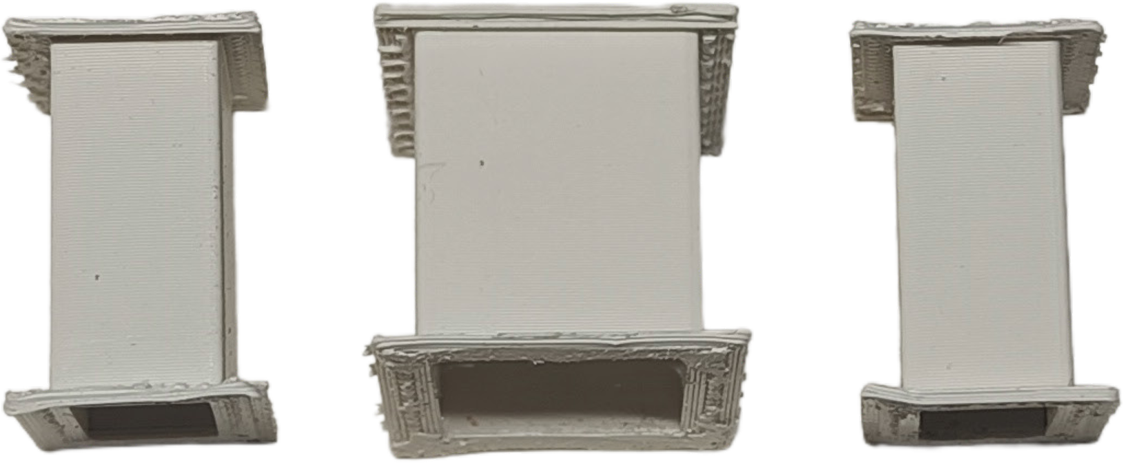
\includegraphics[width=0.54\columnwidth]{Figures_v2/bobbin.pdf}
        \label{fig:bobbin}
        }

        \subfloat[]{
        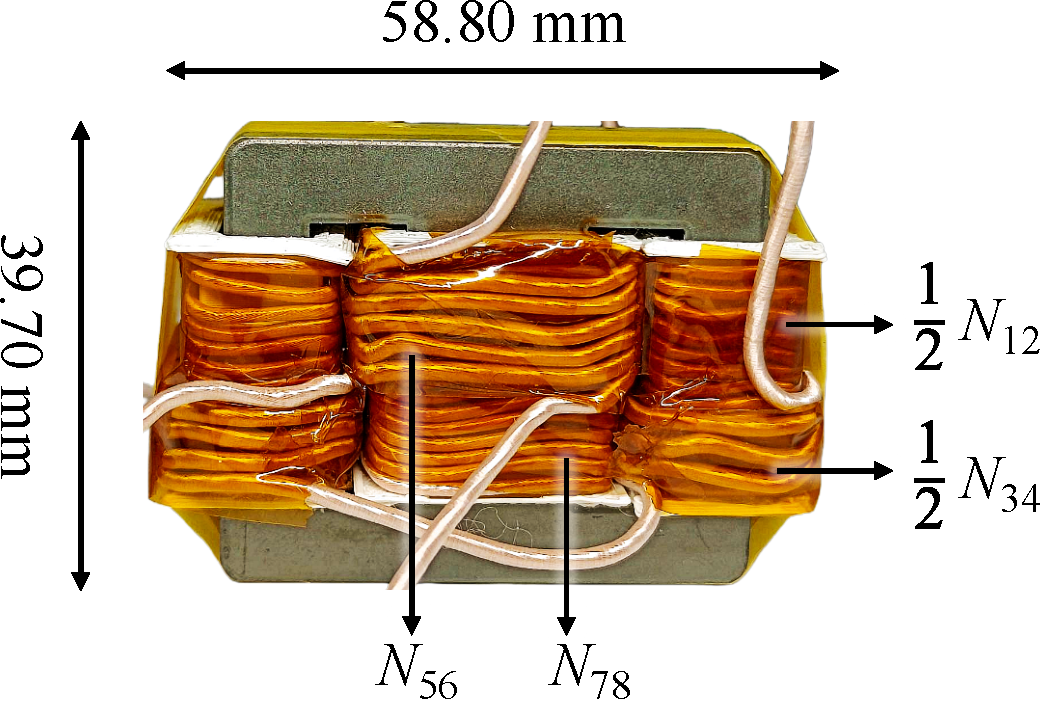
\includegraphics[width=0.7\columnwidth]{Figures_v2/trans.pdf}
        \label{fig:trans}
        }
        
        \caption{Photographs of the proposed integrated transformer: (a) EE-core for the prototype; (b) lab-produced coil formers using a Flashforge Adventurer 4 Series 3D printer; and (c) final assembled prototype, with windings labeled.}
\end{figure}



The comprehensive list of equipment used in the experimental evaluation is summarized in Table~\ref{tab:equipment}. A Tektronix MSO58 high-definition oscilloscope was used to capture experimental waveforms. The open-loop PWM signals were generated via a Tektronix AFG31000 Series function generator, and the integrated transformer parameters were characterized using a Hioki IM3536 LCR meter at 100 kHz.

The coupling coefficients of the transformers $k_{N_{12}-N_{34}}$, $k_{N_{56}-N_{78}}$, and $k_{N_{12}-N_{56}}$ were derived from the mutual inductance obtained after connecting the respective transformer windings in series-aiding and series-opposing configurations. The physical overlapping of the windings resulted in high intra-phase coupling coefficients, with $k_{N_{12}-N_{34}}$ measured at 0.970 and $k_{N_{56}-N_{78}}$ at 0.979. Furthermore, the cross-coupling coefficient between the two flyback transformers $k_{N_{12}-N_{56}}$ is 0.0005, showing that the coupling between phases was almost eliminated. Because this decoupling is geometrically enforced by the core and winding arrangement, it is expected to be maintained even under load transient conditions. While severe transients may introduce high-frequency harmonics that slightly degrade this ideal isolation due to parasitic elements, their magnitude and energy are negligible compared to the fundamental operating frequencies, ensuring that the overall dynamic stability of the converter is preserved.

\begin{table}[b!]
    \caption{Specifications of the Prototype Two-Phase Interleaved Flyback Rectifier}
    \centering
    \footnotesize
    \setlength{\tabcolsep}{3pt} % Slightly tighter spacing to handle long text
    \begin{tabular}{ccc}
        \hline
        \textbf{Item} & \textbf{Symbol} & \textbf{Value / Component} \\
        \hline \hline
        AC input voltage & $v_{\mathrm{in}}$ & 100-240 V$_{\textrm{rms}}$ \\
        Maximum rated power & $P_{\mathrm{O}}$ & 240 W \\
        Output voltage & $V_{\mathrm{O}}$ & 48 V \\
        Switching frequency & $f_{\mathrm{s}}$ & 100 kHz \\
        Bridge diode & $BD$ & CD-DF408S \\
        Input capacitor & $C_{\mathrm{in}}$ & 1 \textmu F \\
        Switch & $S_1, S_2$ & STF15N80k5 \\
        Secondary diode & $D_1, D_2$ & STPSC30H12CWL \\
        Output capacitor & $C_{\mathrm{O}}$ & 2 x 1mF, in parallel \\
        Snubber capacitor & $C_{\mathrm{sn}_1}, C_{\mathrm{sn}_2}$ & 2.2 nF \\
        Snubber resistor & $R_{\mathrm{sn}_1}, R_{\mathrm{sn}_2}$ & 30 k$\Omega$ \\
        Snubber diode & $D_{\mathrm{sn}_1}, D_{\mathrm{sn}_2}$ & VS-E7MH0112-M3/1 \\
        \hline
    \end{tabular}
    \label{tab:prototype_rectifier}
\end{table}

% --- TABLE VII: Transformer Specifications ---
\begin{table}[b!]
    \caption{Specifications of the Prototype Integrated Transformer}
    \centering
    \footnotesize
    \setlength{\tabcolsep}{4pt} 
    \begin{tabular}{ccc}
        \hline
        \textbf{Item} & \textbf{Symbol} & \textbf{Value} \\
        \hline \hline
        Magnetizing inductance (Target) & $L_{\mathrm{m}}$ & 82.8 \textmu H \\
        Magnetizing inductance of $N_{12}-N_{34}$ & $L_{\mathrm{m}_1}$ & 86.1 \textmu H \\
        Magnetizing inductance of $N_{56}-N_{78}$ & $L_{\mathrm{m}_2}$ & 75.1 \textmu H \\
        Turn ratio & $n$ & 3 \\
        Magnetic core & - & OP44721EC \\
        \multirow{2}{*}{Number of turns} & $N_{12}:N_{34}$ & 24:8 \\
                                         & $N_{56}:N_{78}$ & 15:5 \\
        Center leg air gap & $l_{{\mathrm{mc}}_{\mathrm{air}}}$ & 0.650 mm \\
        Outer leg air gap & $l_{{\mathrm{mo}}_{\mathrm{air}}}$ & 0.500 mm \\
        Coupling coefficient of $N_{12}, N_{34}$ & $k_{N_{12}-N_{34}}$ & 0.970 \\
        Coupling coefficient of $N_{56}, N_{78}$ & $k_{N_{56}-N_{78}}$ & 0.979 \\
        Coupling coefficient of $N_{12}, N_{56}$ & $k_{N_{12}-N_{56}}$ & 0.0005 \\
        \hline
    \end{tabular}
    \label{tab:prototype_transformer}
\end{table}

\begin{table}[b!] % You can change [htbp] to [b!] if you want to force it to the bottom of a page
    \caption{Equipment Used in the Experimental Verification}
    \centering
    \footnotesize
    \setlength{\tabcolsep}{3pt}
    \begin{tabular}{cc}
        \hline
        \textbf{Equipment Type} & \textbf{Manufacturer \& Model} \\
        \hline \hline
        AC Power Supply & Kikusui CR2000M \\
        DC Electronic Load & Kikusui PLZ1004WH \\
        Oscilloscope (8-Channel) & Tektronix MSO58 \\
        Differential Voltage Probes & Tektronix THDP0200 \\
        Current Probes & Tektronix TCP0030A \\
        Auxiliary Power Supply (5 V) & Matsusada TB160V15A720W \\
        Auxiliary Power Supply (3.3 V) & Kikusui PWR401L \\
        Function Generator & Tektronix AFG31000 Series \\
        LCR Meter & Hioki IM3536 \\
        \hline
    \end{tabular}
    \label{tab:equipment}
\end{table}

\subsection{Experimental Results}
Fig. \ref{fig:16a} shows the 100 W experimental waveforms at 4 ms/div from the two-phase interleaved flyback rectifier with the proposed transformer, demonstrating PFC. Fig. \ref{fig:16b} presents 2 \textmu s/div waveforms. No current is induced in either switch except during the resonance between the leakage inductance and the parasitic capacitance of the switch. During the inactive period of the transformer, secondary diode side current is zero. Moreover, after $i_{\mathrm{S}_1}$ and $i_{\mathrm{S}_2}$ reached zero when $S_1$ and $S_2$ switched off, the currents remained at zero. Therefore, the two flyback converters operate independently without magnetic coupling interference. The same phenomenon was observed at 240 W two-phase drive, as shown in Fig. \ref{fig:16c}. Single-phase drive at lower power at 32.5 W is also feasible as shown in Fig. \ref{fig:16d}.
\begin{figure}[htbp]
\centering
% (a) Top circuit
        \subfloat[]{
        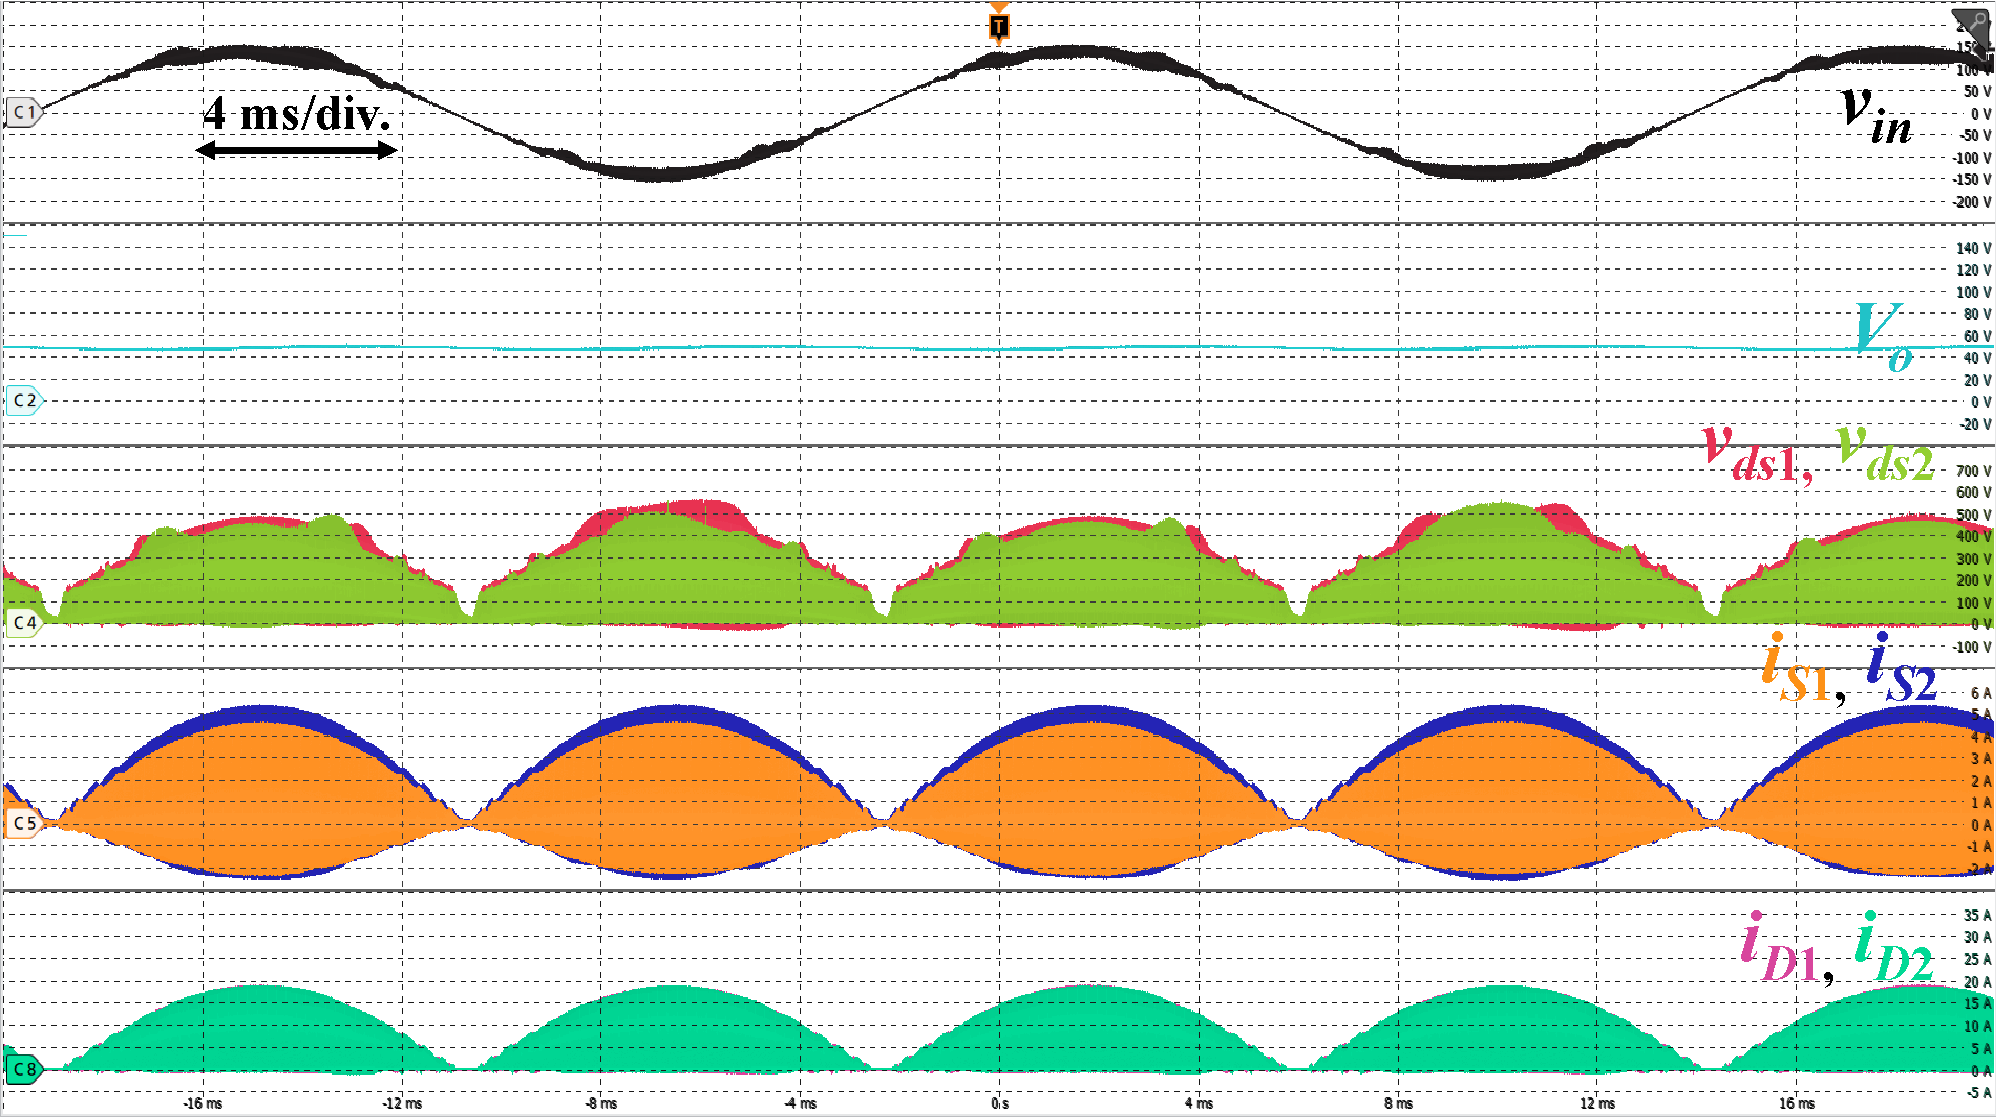
\includegraphics[width=0.95\columnwidth]{Figures_v2/Fig16a.pdf} % Make sure this file exists
        \label{fig:16a}}
        \\ % This double backslash forces the next image to the line below (vertical stack)
        % (b) Middle circuit
        \subfloat[]{
        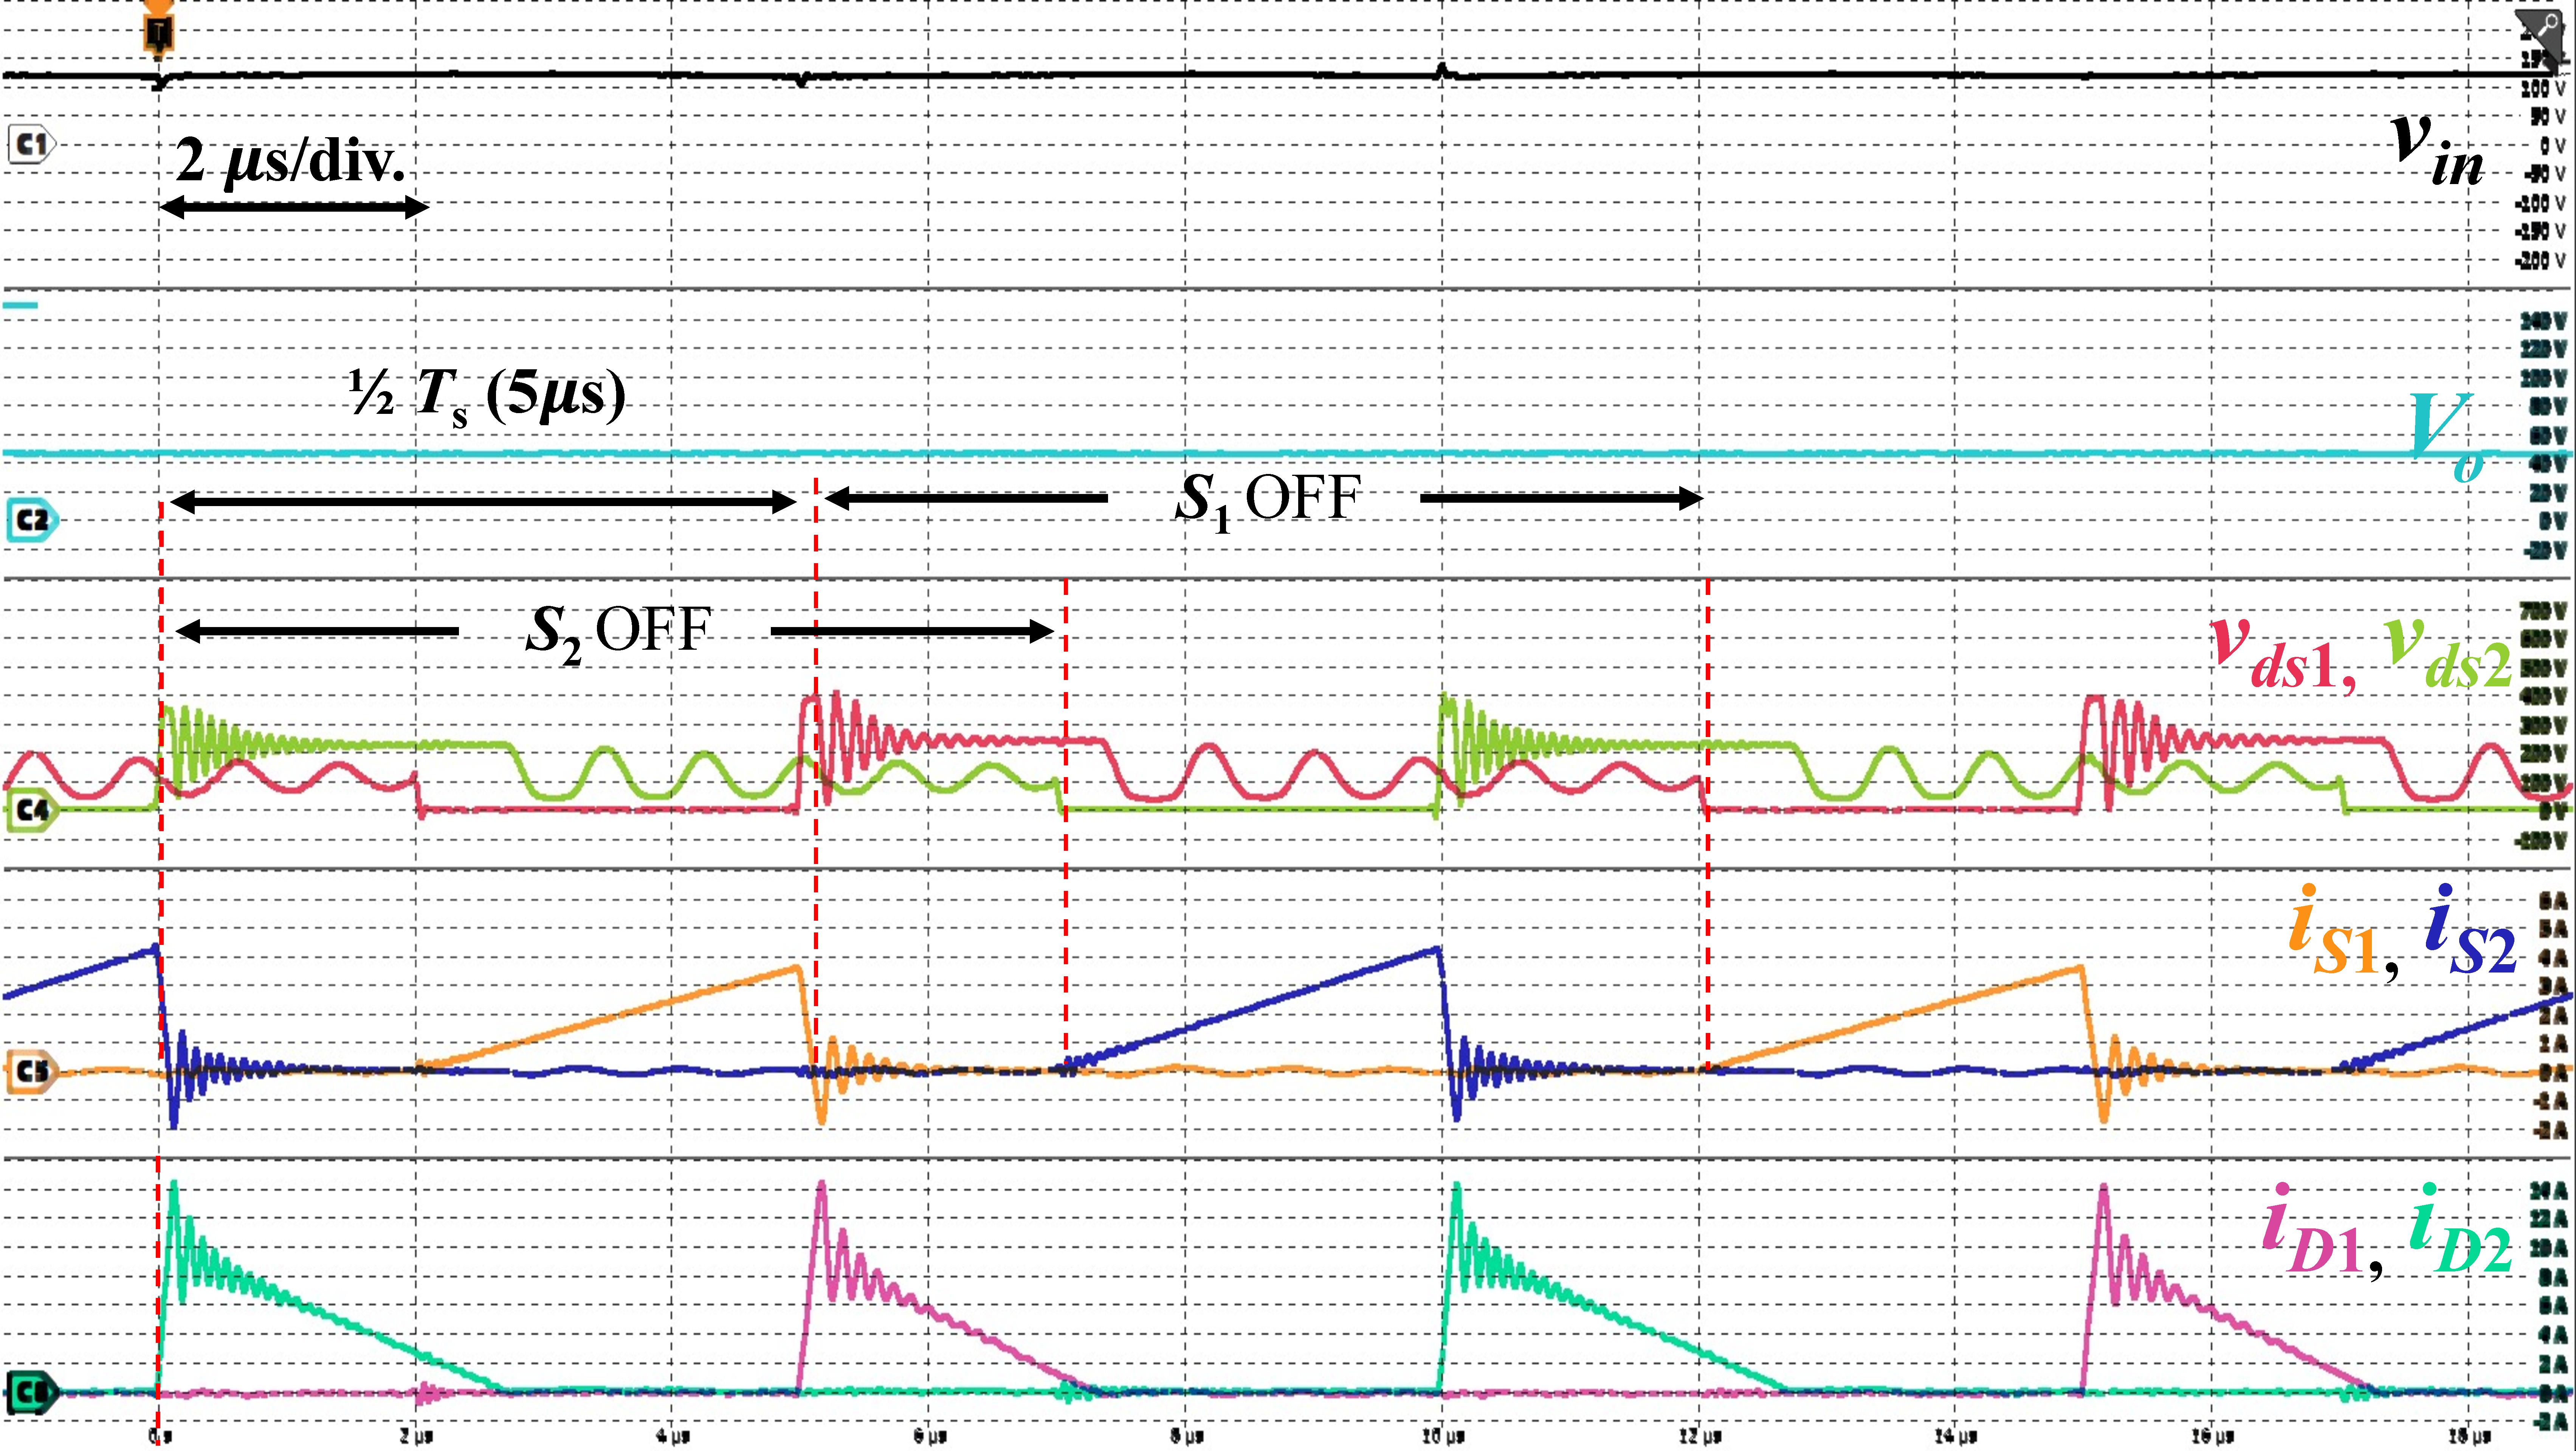
\includegraphics[width=0.95\columnwidth]{Figures_v2/Fig16b.pdf}
        \label{fig:16b}}
        \\ % This double backslash forces the next image to the line below (vertical stack)
        % (b) Middle circuit
        \subfloat[]{
        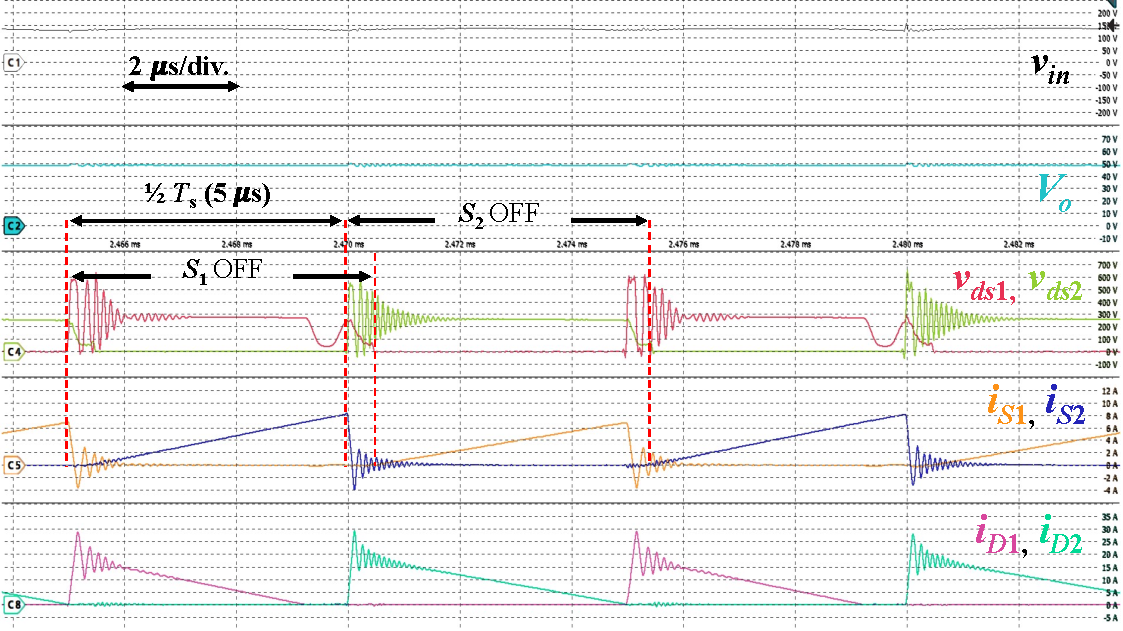
\includegraphics[width=0.95\columnwidth]{Figures_v2/Fig16c.pdf}
        \label{fig:16c}}
        \\ % This double backslash forces the next image to the line below (vertical stack)
        % (b) Middle circuit
        \subfloat[]{
        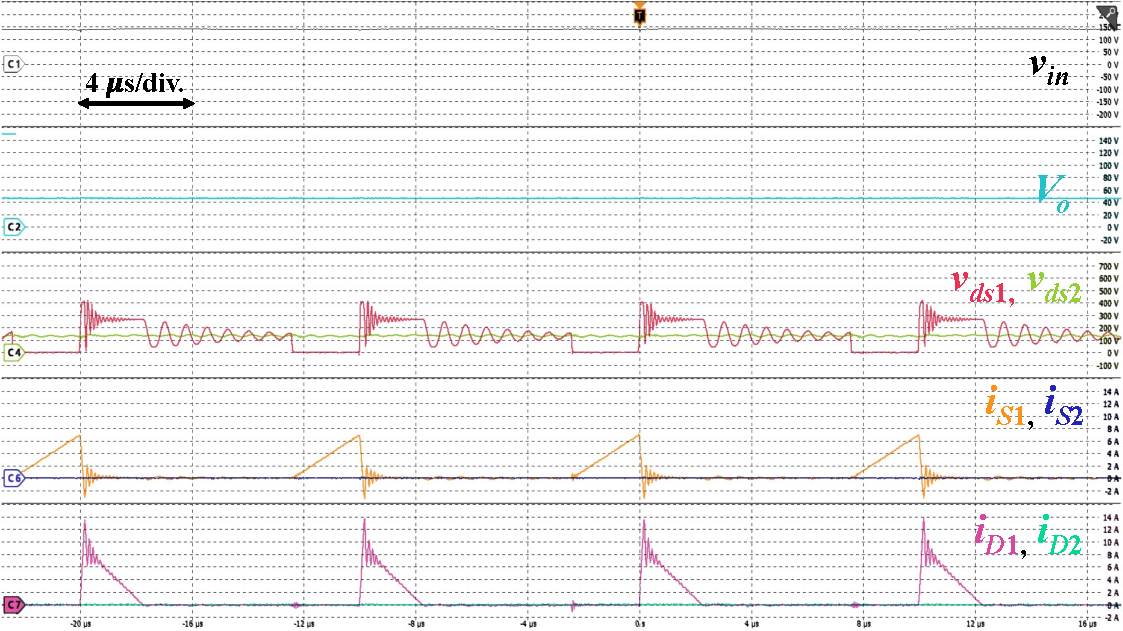
\includegraphics[width=0.95\columnwidth]{Figures_v2/Fig16d.pdf}
        \label{fig:16d}}
        
        \caption{Experimental waveforms of the proposed two-phase interleaved flyback rectifier at (a) \& (b): 100 W, two-phase AC drive, (c): 240 W, two-phase AC drive, (d): 32.5 W, single-phase AC drive. For (a) and (b): $v_{\mathrm{in}}$: 50 V/div., $V_{\mathrm{o}}$: 10 V/div., $v_{\mathrm{ds}_1}, v_{\mathrm{ds}_2}$: 100 V/div., $i_{\mathrm{S}_1}, i_{\mathrm{S}_2}$: 1 A/div., $i_{\mathrm{D}_1}, i_{\mathrm{D}_2}$: 5 A/div.; For (c): $v_{\mathrm{in}}$: 50 V/div., $V_{\mathrm{o}}$: 10 V/div., $v_{\mathrm{ds}1}, v_{\mathrm{ds}2}$: 100 V/div., $i_{\mathrm{S}_1}, i_{\mathrm{S}_2}$: 2 A/div., $i_{\mathrm{D}_1}, i_{\mathrm{D}_2}$: 5 A/div.; For (d): $v_{\mathrm{in}}$: 50 V/div., $V_{\mathrm{o}}$: 20 V/div., $v_{\mathrm{ds}_1}, v_{\mathrm{ds}_2}$: 100 V/div., $i_{\mathrm{S}_1}, i_{\mathrm{S}_2}$: 2 A/div., $i_{\mathrm{D}_1}, i_{\mathrm{D}_2}$: 2 A/div.}
        \label{fig:16}
\end{figure}

Two distinct parasitic resonant behaviors can be observed in the $v_\mathrm{ds}$ waveforms in Fig.~\ref{fig:16b} and Fig.~\ref{fig:16c} according to the operational dynamics of the flyback converter. The same phenomenon can also be observed in Fig.~\ref{fig:16d} for one-phase drive. A high-frequency ringing occurs immediately at switch turn-off, driven by the resonance between the leakage inductance of the transformer and the parasitic output capacitance $C_\mathrm{oss}$ of the switches. This voltage stress is mitigated by the implemented primary-side RCD snubbers. Second, a lower-frequency oscillation appears when the secondary diode currents $i_{\mathrm{D}_1}$ and $i_{\mathrm{D}_2}$ reach zero, indicating complete transformer demagnetization. During this interval, the main magnetizing inductance of the active transformer resonates with $C_\mathrm{oss}$ until the next switching cycle initiates. Nevertheless, these parasitic behaviors do not interfere with the non-coupled operation of the proposed transformer.

% --- TABLE VI: Rectifier Specifications ---





\section{Conclusion}
In this paper, an integrated transformer was successfully designed for a two-phase interleaved flyback rectifier for USB PD applications. The proposed winding structure for the integrated transformer prevents coupling between the two flyback transformers and achieves simple manufacturability through the use of a commercial EE-core. A coupling coefficient of 0.0005 was achieved with the prototype. Independent flyback circuit operation without magnetic interference due to coupling was verified through simulation and experiment up to 240 W. Through the proposed design, two discrete transformers are integrated into a single magnetic component. The structure is estimated to enable up to a 16\% downsizing of magnetic components compared to conventional discrete transformers.

% --- TABLE V: Volume Analysis ---




% --- TABLE VII: Transformer Specifications ---
% --- TABLE VII: Transformer Specifications ---


\begin{thebibliography}{1}
\bibliographystyle{IEEEtran}

\bibitem{ref1}
A. Medina-Garcia, J. Cruz-Cozar, D. P. Morales-Santos, N. Rodriguez, and M. Schlenk, "A high-efficiency isolated wide voltage range DC-DC converter using WBG devices," \textit{IEEE Access}, vol. 10, pp. 84818-84825, Aug. 2022.

\bibitem{ref2}
USB-IF PR, "USB Promoter Group announces USB Power Delivery specification revision 3.1," 2021. [Online]. Available: https://www.usb.org/sites/default/files/2021-05/USB\%20PG\%20USB\%20PD\%203.1\%20DevUpdate\%20\\Announcement\_FINAL.pdf

\bibitem{ref2.2}
D. Waters, ``Power System Implications of the New USB Power Delivery 3.2,'' in \textit{Proc. IEEE Appl. Power Electron. Conf. Expo. (APEC)}, 2024. [Presentation Slides].

\bibitem{ref6}
X. Huang, J. Feng, W. Du, F. C. Lee, and Q. Li, "Design consideration of MHz active clamp flyback converter with GaN devices for low power adapter application," in \textit{Proc. IEEE Appl. Power Electron. Conf. Expo. (APEC)}, 2016, pp. 2334-2341.

\bibitem{ref7}
J. Zhang, X. Huang, X. Wu, and Z. Qian, "A high efficiency flyback converter with new active clamp technique," \textit{IEEE Trans. Power Electron.}, vol. 25, no. 7, pp. 1775-1785, Feb. 2010.


\bibitem{ref8}
J. Shin, S. Choi, and B. Cho, "High-efficiency bridgeless flyback rectifier with bidirectional switch and dual output windings," \textit{IEEE Trans. Power Electron.}, vol. 29, no. 9, pp. 4752-4762, Oct. 2013.

\bibitem{ref9}
S. Choi, Y. Yin, J.-W. Shin, J. Imaoka, and M. Yamamoto, "Common-mode noise reduction for bridgeless flyback PFC rectifier with balance technique," in \textit{Proc. IEEE Appl. Power Electron. Conf. Expo. (APEC)}, 2024, pp. 1478-1483.

\bibitem{ref10}
K. T. Mok, Y. M. Lai, and K. H. Loo, "A single-stage bridgeless power-factor-correction rectifier based on flyback topology," in \textit{Proc. IEEE 33rd Int. Telecommun. Energy Conf. (INTELEC)}, 2011, pp. 1-6.

\bibitem{ref11}
J. Beak, J. Shin, P. Jang, and B. Cho, "A critical conduction mode bridgeless flyback converter," in \textit{Proc. 8th Int. Conf. Power Electron. - ECCE Asia}, 2011, pp. 487-492.

\bibitem{ref3}
B. C. Kim, K. B. Park, C. E. Kim, B. H. Lee, and G. W. Moon, "LLC resonant converter with adaptive link-voltage variation for a high-power-density adapter," \textit{IEEE Trans. Power Electron.}, vol. 25, no. 9, pp. 2248-2252, May 2010.

\bibitem{ref4}
Y. C. Lin, F. C. Lee, Q. Li, X. Huang, and Z. Lin, "A novel AC-to-DC adaptor with ultra-high power density and efficiency," in \textit{Proc. IEEE Appl. Power Electron. Conf. Expo. (APEC)}, 2016, pp. 1853-1860.

\bibitem{ref5}
M. Li, Z. Ouyang, and M. A. E. Andersen, "Analysis and optimal design of high-frequency and high-efficiency asymmetrical half-bridge flyback converters," \textit{IEEE Trans. Ind. Electron.}, vol. 67, no. 10, pp. 8312-8321, Nov. 2019.

\bibitem{ref12}
B. Shafer, "Interleaving contributes unique benefits to forward converters and flyback converters," in \textit{Texas Instruments Power Supply Design Seminar}, Topic, vol. 4, pp. 1-32, 2004.

\bibitem{Su_2013}
J.-T. Su and C.-W. Liu, "A novel phase-shedding control scheme for improved light load efficiency of multiphase interleaved DC-DC converters," \textit{IEEE Trans. Power Electron.}, vol. 28, no. 10, pp. 4742-4752, Oct. 2013.

\bibitem{Zhang_2013}
Y. Zhang, X.-F. He, Z. Zhang, and Y.-F. Liu, "A hybrid control method for photovoltaic grid-connected interleaved flyback micro-inverter to achieve high efficiency in wide load range," in \textit{Proc. IEEE Appl. Power Electron. Conf. Expo. (APEC)}, 2013, pp. 751-756.

\bibitem{Chen_2014}
H.-C. Chen, "Interleaved current sensorless control for multiphase boost-type switch-mode rectifier with phase-shedding operation," \textit{IEEE Trans. Ind. Electron.}, vol. 61, no. 2, pp. 766-775, Feb. 2014.

\bibitem{Yang_2020}
F. Yang, C. Li, Y. Cao, and K. Yao, "Two-phase interleaved boost PFC converter with coupled inductor under single-phase operation," \textit{IEEE Trans. Power Electron.}, vol. 35, no. 1, pp. 169-184, Jan. 2020.

\bibitem{Z_Li_2025}
Z. Li, J. Liang, M. Fu, T. Long, and H. Wang, "Nonlinear coupled inductor-based light-load efficiency boost technique for trans-inductor voltage regulators," \textit{IEEE Trans. Power Electron.}, vol. 40, no. 10, pp. 14368-14373, Oct. 2025.

\bibitem{meng2021}
T. Meng, H. Ben, C. Li, and F. Wu, "Investigation of the integrated-transformer winding architectures in the input-series flyback auxiliary power supply considering the stray capacitances," \textit{IEEE Trans. Power Electron.}, vol. 36, no. 2, pp. 1790-1803, Feb. 2021.

\bibitem{kwon2024}
G.-H. Kwon, D.-I. Lee, S.-W. Jeong, and H.-S. Youn, "Next-generation active-clamp forward-flyback converter with integrated planar transformer for 4 kW LDC," \textit{IEEE Access}, vol. 13, pp. 2449-2462, 2025.

\bibitem{Ahmad}
U. Ahmad, H. Cha, and N. Naseem, "Integrated current balancing transformer based input-parallel output-parallel LLC resonant converter modules," \textit{IEEE Trans. Power Electron.}, vol. 36, no. 5, pp. 5278-5289, May 2021.

\bibitem{Dou}
Y. Dou, Z. Ouyang, and M. A. E. Andersen, "Integrated coupled inductors with functionality of current balancing transformer for two-phase synchronous DC-DC converters," \textit{IEEE Trans. Power Electron.}, vol. 35, no. 5, pp. 4472-4476, May 2020.

\bibitem{Nakakohara}
Y. Nakakohara, H. Otake, T. M. Evans, T. Yoshida, M. Tsuruya, and K. Nakahara, "Three-phase LLC series resonant DC/DC converter using SiC MOSFETs to realize high-voltage and high-frequency operation," \textit{IEEE Trans. Ind. Electron.}, vol. 63, no. 4, pp. 2103-2110, Apr. 2016.

\bibitem{Z_Chen_s42835}
Z. Chen, L. Shen, and Y. Wu, "An improved interleaved flyback converter with reduced voltage stress and current auto-sharing," \textit{J. Electr. Eng. Technol.}, vol. 19, pp. 2251-2263, Nov. 2023.

\bibitem{shi2024}
Y. Shi, Y. Xu, Y. Yang, F. Wang, and C. Xu, "A DCM interleaved flyback micro-inverter with new auxiliary active clamp branch design for zero-voltage switching effect," in \textit{Proc. Energy Convers. Congr. Expo. Europe (ECCE Europe)}, 2024, pp. 1-6.

\bibitem{cheng2018}
M.-H. Cheng, T.-J. Liang, W.-Y. Huang, and W.-C. Yang, "Interleaved half-bridge flyback converter with zero-voltage switching," in \textit{Proc. IEEE Energy Convers. Congr. Expo. (ECCE)}, 2018, pp. 5967-5973.

\bibitem{wu2015}
C.-H. Wu \textit{et al.}, "Design and implementation of a novel interleaved flyback converter with leakage energy recycled," in \textit{Proc. IEEE Energy Convers. Congr. Expo. (ECCE)}, 2015, pp. 5888-5895.

\bibitem{cheng2023}
J. Cheng, T. Liang, K. Liao, and K. Chen, "Design and implementation of interleaved flyback converter with GaN E-HEMT," in \textit{Proc. IEEE Appl. Power Electron. Conf. Expo. (APEC)}, 2023, pp. 2474-2480.

\bibitem{mayer2025}
R. Mayer, L. S. de Oliveira, M. B. E. Kattel, L. C. Gili, and S. V. G. Oliveira, "An interleaved forward/flyback DC–DC converter with bidirectional capability and wide voltage range characteristic," \textit{IEEE Trans. Power Electron.}, vol. 40, no. 8, pp. 11051-11063, Aug. 2025.

\bibitem{ishihara2015}
M. Ishihara, S. Kimura, W. Martinez, and M. Yamamoto, "Analysis and design of passive components for interleaved flyback converter with integrated transformer," in \textit{Proc. IEEE Energy Convers. Congr. Expo. (ECCE)}, 2015, pp. 5902-5909.

\bibitem{tonolo2025}
É. A. Tonolo, J. W. M. Soares, and A. A. Badin, "An interleaved current-fed PFC flyback converter with voltage follower characteristic," \textit{IEEE Open J. Power Electron.}, vol. 7, pp. 118-127, 2026.

\bibitem{qian2008}
T. Qian and B. Lehman, "Coupled input-series and output-parallel dual interleaved flyback converter for high input voltage application," \textit{IEEE Trans. Power Electron.}, vol. 23, no. 1, pp. 88-95, Jan. 2008.

\bibitem{Mao_2011}
C.-f. Mao, W. Chen, and Z.-y. Lu, "Small signal analysis of interleaved flyback converter with magnetic integration," \textit{Adv. Technol. Electr. Eng. Energy}, vol. 30, no. 4, pp. 26-29, Oct. 2011.

%\bibitem{Jin_2024}
%F. Jin, T. Yuan, A. Nabih, and Q. Li, "Efficient integrated magnetics with winding cancellation technique to reduce common-mode EMI noise for a single-phase CLLC converter," \textit{IEEE Trans. Power Electron.}, vol. 39, no. 11, pp. 14758-14774, Nov. 2024.

\bibitem{Ouyang}
Z. Ouyang, Z. Zhang, M. A. E. Andersen, and O. C. Thomsen, "Four quadrants integrated transformers for dual-input isolated DC-DC converters," \textit{IEEE Trans. Power Electron.}, vol. 27, no. 6, pp. 2697-2702, Jun. 2012.

\bibitem{fayyaz2025}
S. Fayyaz \textit{et al.}, "Higher power density decoupled magnetic device with core integrated orthogonal windings for power converters," \textit{IEEE Trans. Power Electron.}, vol. 40, no. 4, pp. 5595-5608, Apr. 2025.


\bibitem{ECCE}
H. Hirasawa, K. R. D. Roque, S. Choi, Y. Yonezawa, J. Imaoka and M. Yamamoto, "Design Method of an Integrated Transformer for a Two-Phase Interleaved Flyback PFC Rectifier," in \textit{Proc. IEEE Energy Convers. Congr. Expo. (ECCE)}, 2024, pp. 6650-6656.

\bibitem{ref15}
G. B. Koo, "Design guidelines for RCD snubber of flyback converters," Fairchild Semiconductor, San Jose, CA, USA, Appl. Note AN-4147 Rev. 1.1.0, 2006.

\bibitem{ref16}
W. McMurray, "Selection of snubbers and clamps to optimize the design of transistor switching converters," \textit{IEEE Trans. Ind. Appl.}, vol. IA-16, no. 4, pp. 513-523, 1980.

\bibitem{ref21}
W. Colonel and T. McLyman, \textit{Transformer and Inductor Design Handbook}. Boca Raton, FL, USA: CRC Press, 2004.

\bibitem{ref22}
S. Kimura, S. Aoto, M. Ishihara, J. Imaoka, and M. Yamamoto, "Interleaved active clamp forward converter with novel integrated magnetic components," in \textit{Proc. IEEE Energy Convers. Congr. Expo. (ECCE)}, 2015, pp. 6029-6036.

\end{thebibliography}

%
%\begin{IEEEbiography}[{
\includegraphics[width=1in,height=1.25in,clip,keepaspectratio]{Figures_v2/karlphoto.jpg}}]{Karl Raymond Dela Cruz Roque}
%(Graduate Student Member, IEEE) is with the Graduate School of Engineering, Department of Electrical Engineering, in Nagoya University, Japan. 
%He received the B.Eng. Degree in Automotive Engineering with a Specialization in Electrical Engineering from Nagoya University in Nagoya, Japan in 2024. He is currently pursuing the M.Eng. Degree in Electrical Engineering at Nagoya University, Nagoya, Japan. Since 2023, he has been a Research Assistant at the Nagoya University Yamamoto Laboratory for Power Electronics. His research interests include the design of magnetic components, particularly integrated magnetics and thermal management, as well as resonant converters, control design, and system modeling.%
%\end{IEEEbiography}
%###
%
% Placeholder for other biographies if needed
\vfill

\end{document}